
Se realizaron dos encuestas sobre la aplicación. La primera fue aplicada a más de 50 estudiantes de la carrera de Ingeniería en Sistemas de la Universidad del Valle, quienes respondieron después de probar la aplicación. La segunda encuesta se dirigió a expertos y personas con experiencia en el campo de sistemas, utilizando una evaluación basada en las heurísticas de Nielsen. A continuación, se presentan los resultados junto con un breve análisis de los mismos.
\section{Cuestionario sobre evaluación de experiencia en softskills para los módulos Mindset y Fitness}
\subsection{Fitness: Juego sobre movimiento de la muñeca}
La pregunta ``El juego es fácil de entender y aprender`` obtuvo la mayor cantidad de respuestas en la opción 4, con 29 votos. Esto indica que el juego es relativamente sencillo de comprender, pero aún tiene margen de mejora. La observación más común fue que la posición en ángulo recto de la palma puede resultar un poco confusa.

    \begin{figure}[H]
  \centering
  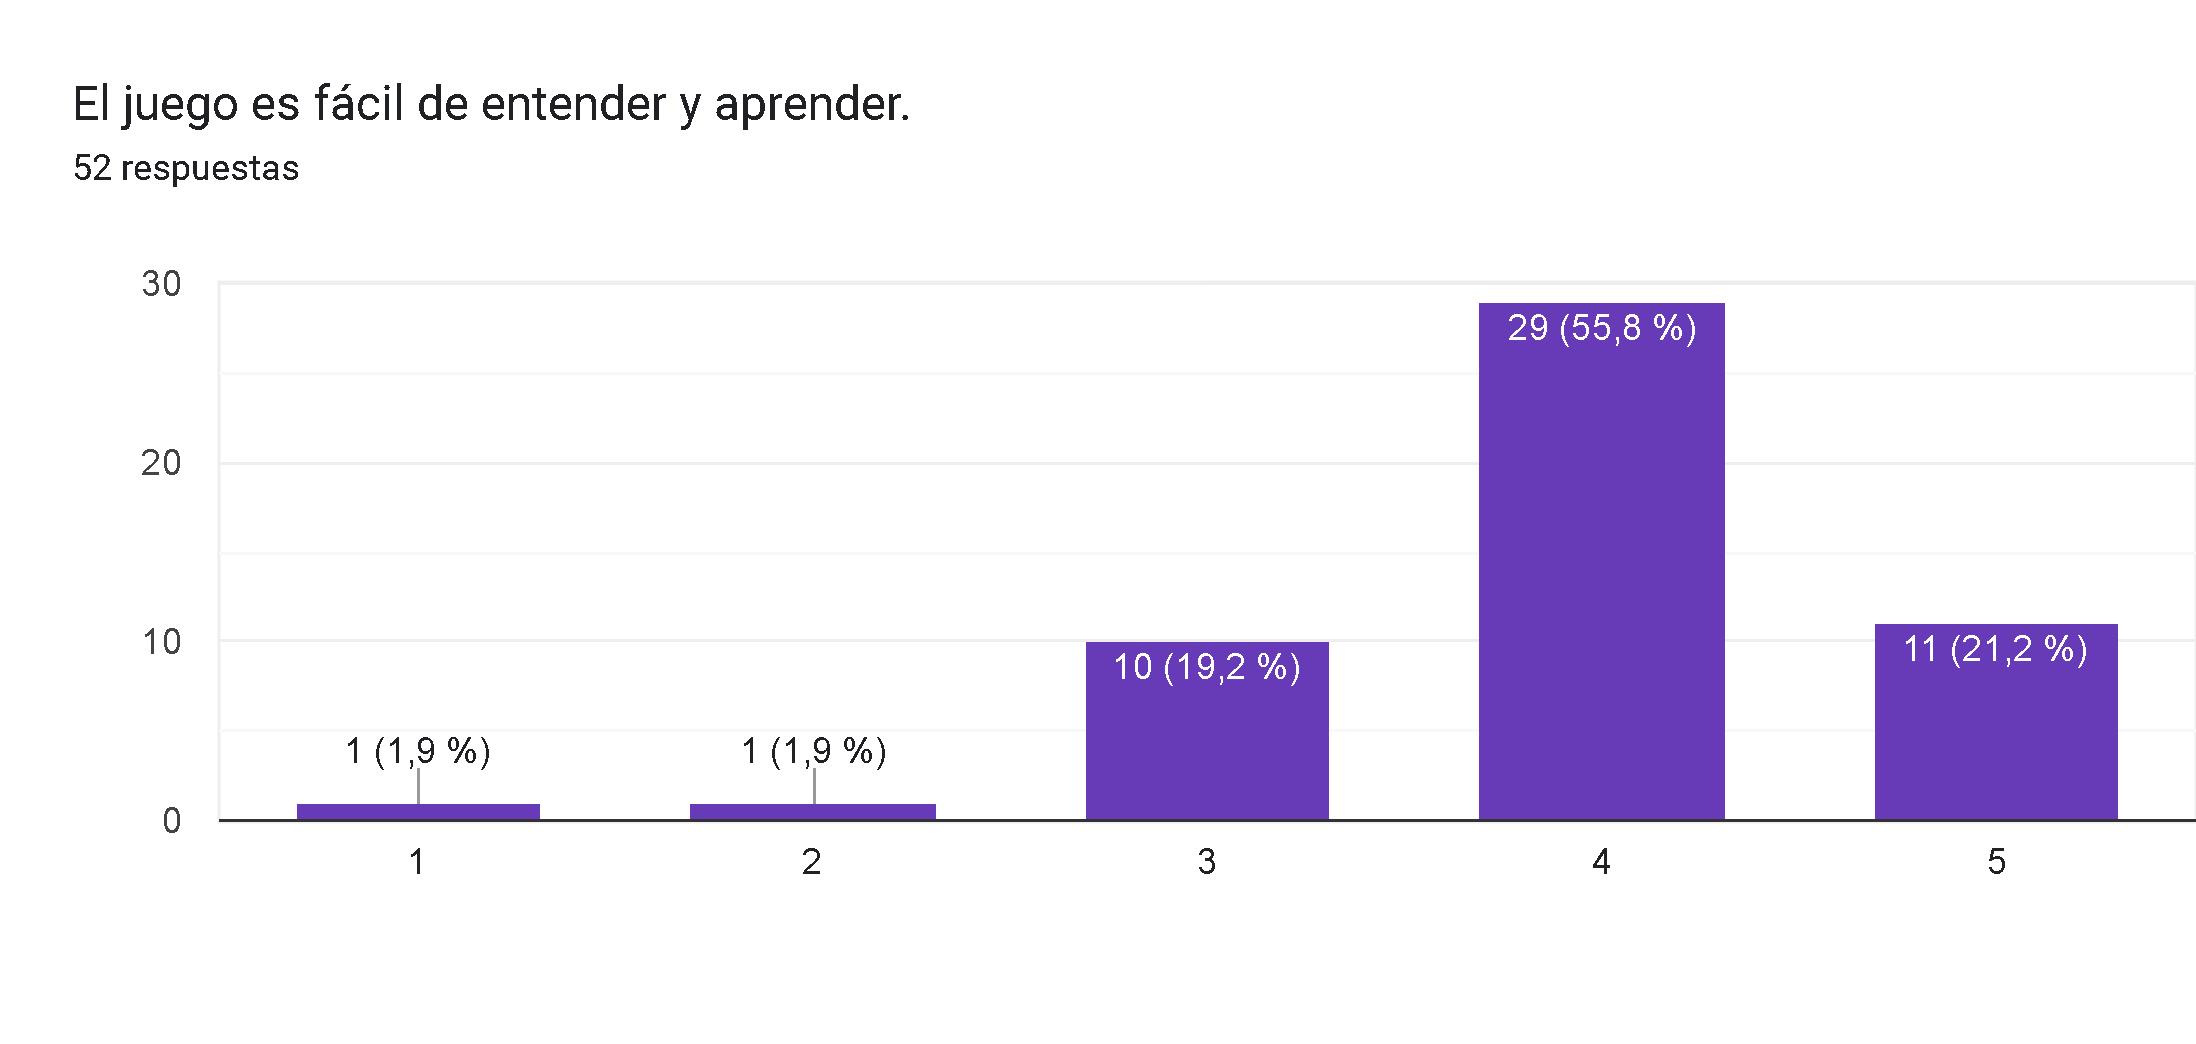
\includegraphics[width=0.7\linewidth]{Imagenes/fc1.png}
  \caption{Elaboración propia, Módulo fitness, Imagen de referencia sobre cuestionario  de gamificación para el módulo fitness del juego sobre la muñeca, ``El juego es fácil de entender y aprender``}
  \label{fig:cuestionario1fitness}
\end{figure}



La pregunta ``Los controles son intuitivos y responden bien`` obtuvo la mayor cantidad de respuestas en la opción 4, con un 40,4 \%. Esto sugiere que los controles son mayormente funcionales e intuitivos, aunque aún hay oportunidad de optimización para una experiencia más fluida.

    \begin{figure}[H]
  \centering
  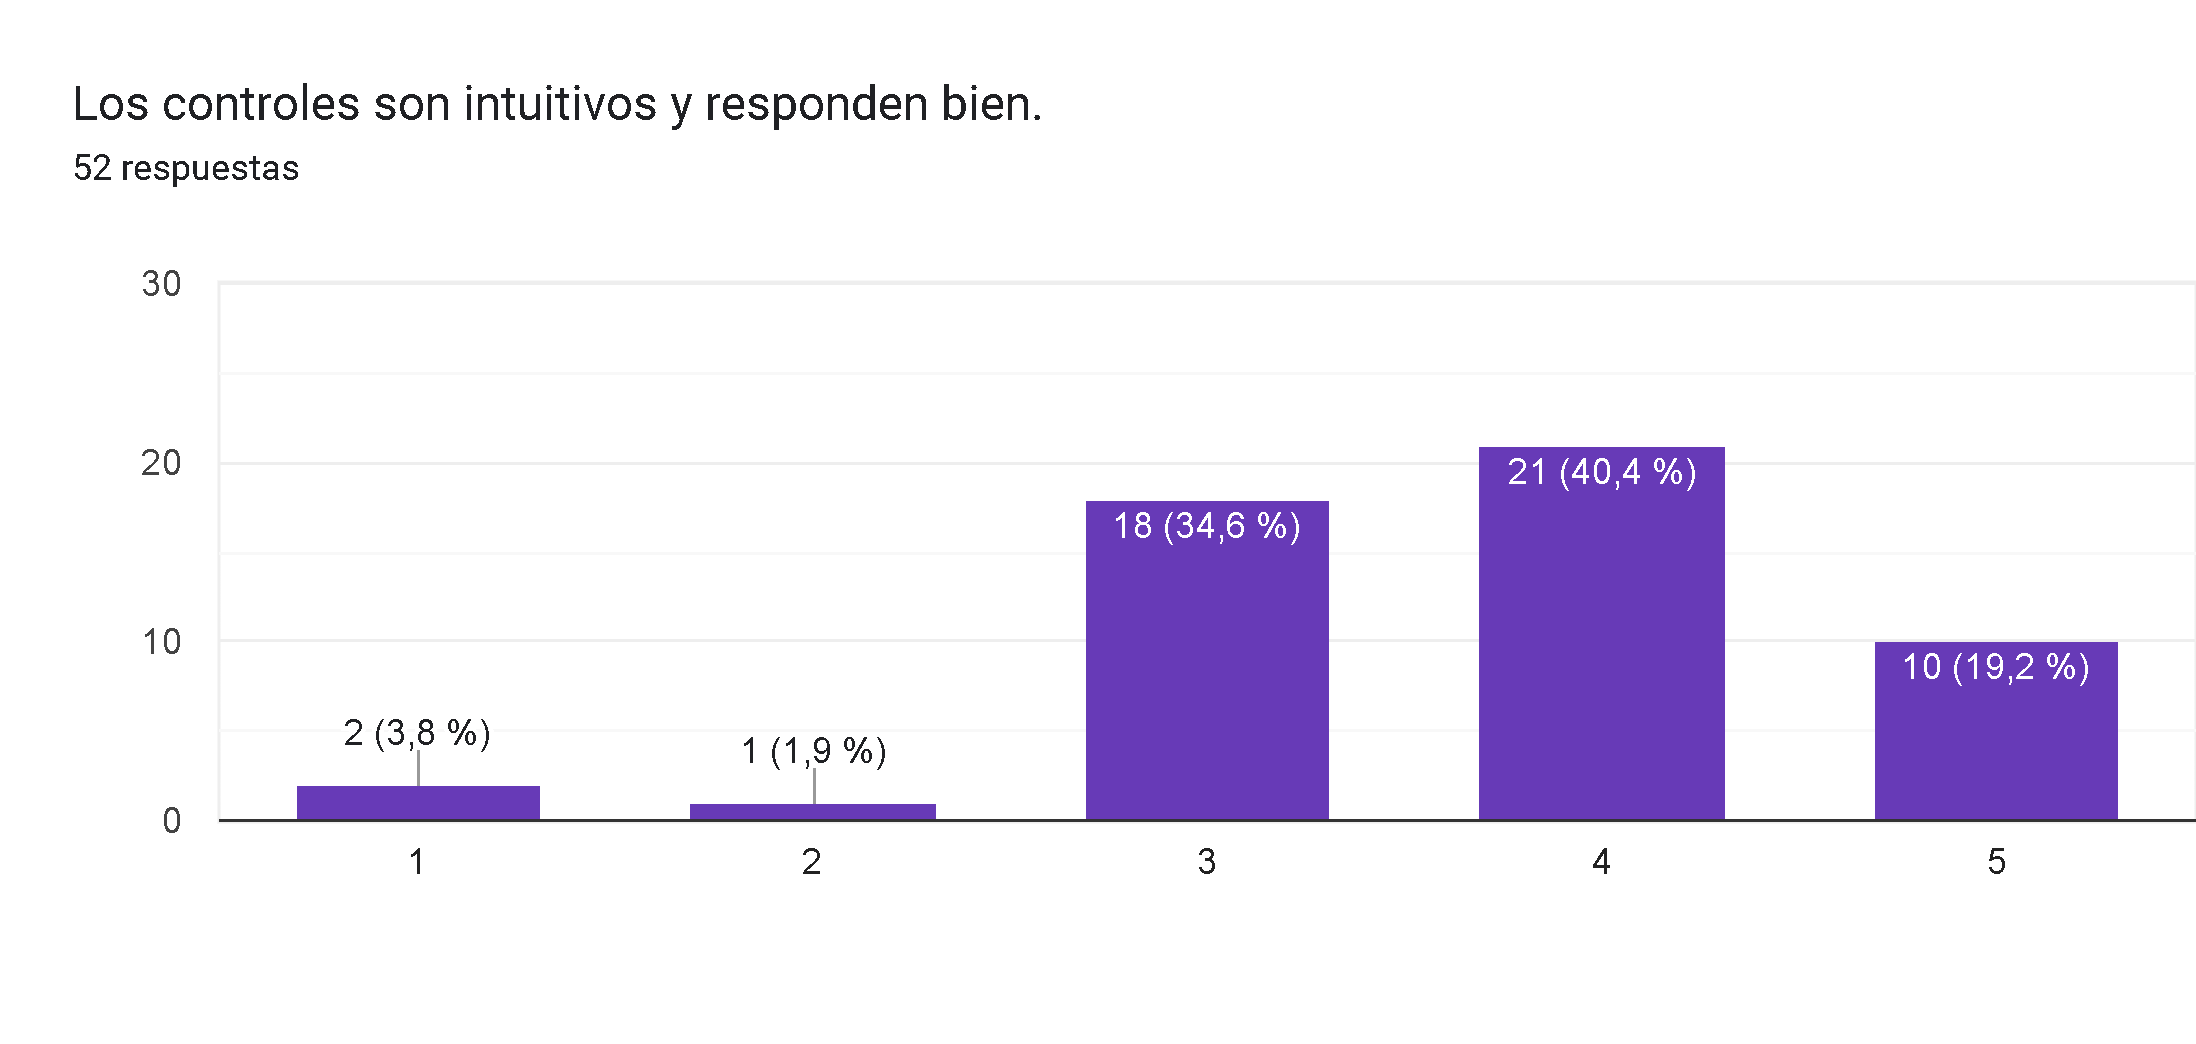
\includegraphics[width=0.7\linewidth]{Imagenes/fc2.png}
  \caption{Elaboración propia, Módulo fitness, Imagen de referencia sobre cuestionario  de gamificación para el módulo fitness del juego sobre la muñeca,  ``Los controles son intuitivos y responden bien``}
  \label{fig:cuestionario2fitness}
\end{figure}
La pregunta ``El nivel de dificultad es adecuado`` obtuvo la mayor cantidad de respuestas en la opción 4, con un 57,7 \%. Esto sugiere que la mayoría de los usuarios considera que la dificultad está bien equilibrada, aunque una parte significativa podría encontrarla demasiado fácil o desafiante.

 \begin{figure}[H]
  \centering
  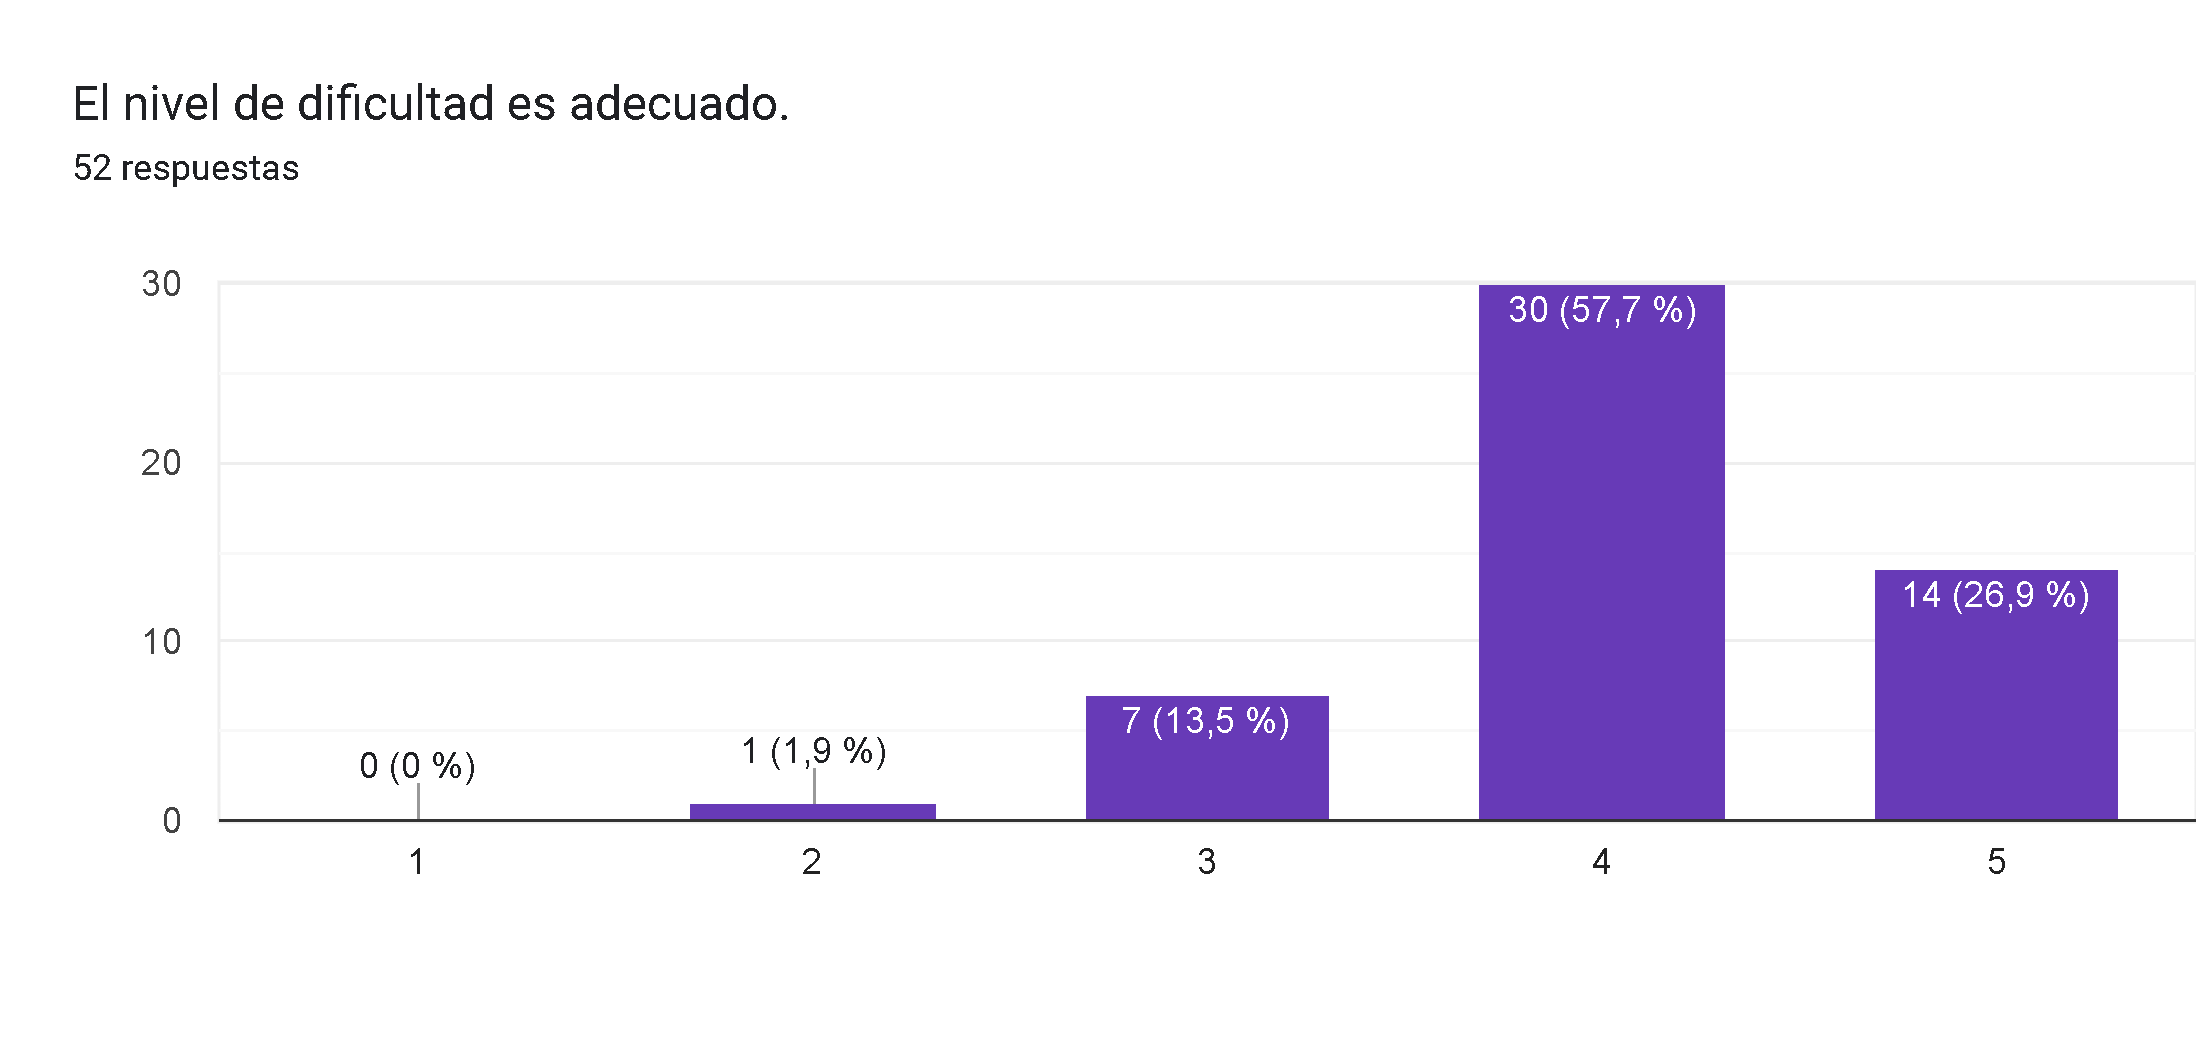
\includegraphics[width=0.7\linewidth]{Imagenes/fc3.png}
  \caption{Elaboración propia, Módulo fitness, Imagen de referencia sobre cuestionario  de gamificación para el módulo fitness del juego sobre la muñeca,  ``El nivel de dificultad es adecuado``}
  \label{fig:cuestionario3fitness}
\end{figure}

La pregunta ``El juego detecta mis movimientos corporales de manera precisa`` obtuvo 20 votos en la opción 3 y 20 en la opción 4, reflejando un puntaje medio. Una observación recurrente fue que la cámara no detecta correctamente la mano si esta lleva un guante de un color similar al fondo. No obstante, dado que no obtuvo una calificación baja, se considera satisfactorio, aunque con posibilidades de mejora.


    \begin{figure}[H]
  \centering
  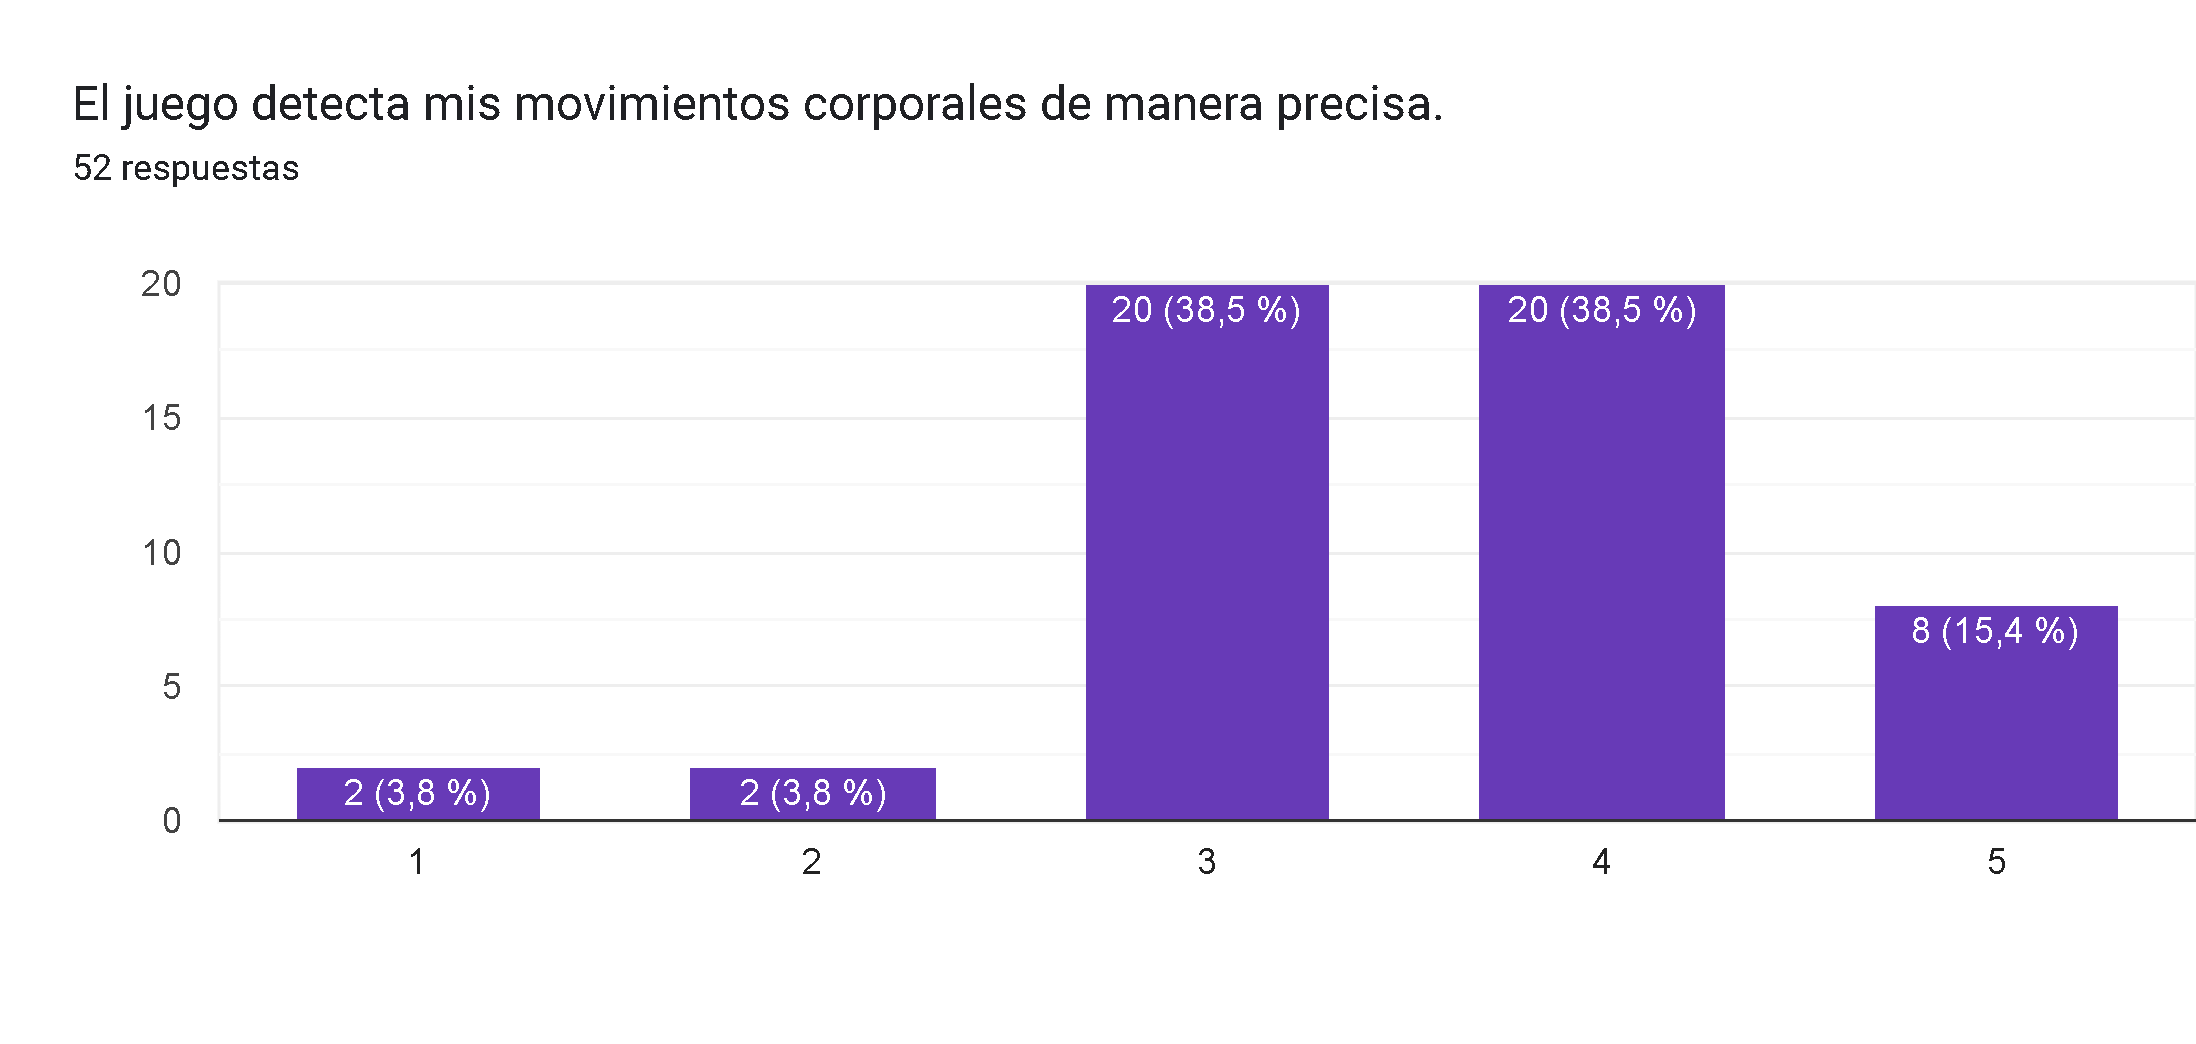
\includegraphics[width=0.7\linewidth]{Imagenes/fc4.png}
  \caption{Elaboración propia, Módulo fitness, Imagen de referencia sobre cuestionario  de gamificación para el módulo fitness del juego sobre la muñeca, ``El juego detecta mis movimientos corporales de manera precisa``}
  \label{fig:cuestionario4fitness}
\end{figure}

La pregunta ``Los movimientos requeridos no provocan fatiga o molestias físicas`` tuvo una respuesta muy positiva, con 24 votos en la opción 5 y ninguno en la opción 1. Esto indica que los movimientos no generaron problemas físicos en la audiencia, siendo bien recibidos por los participantes.

    \begin{figure}[H]
  \centering
  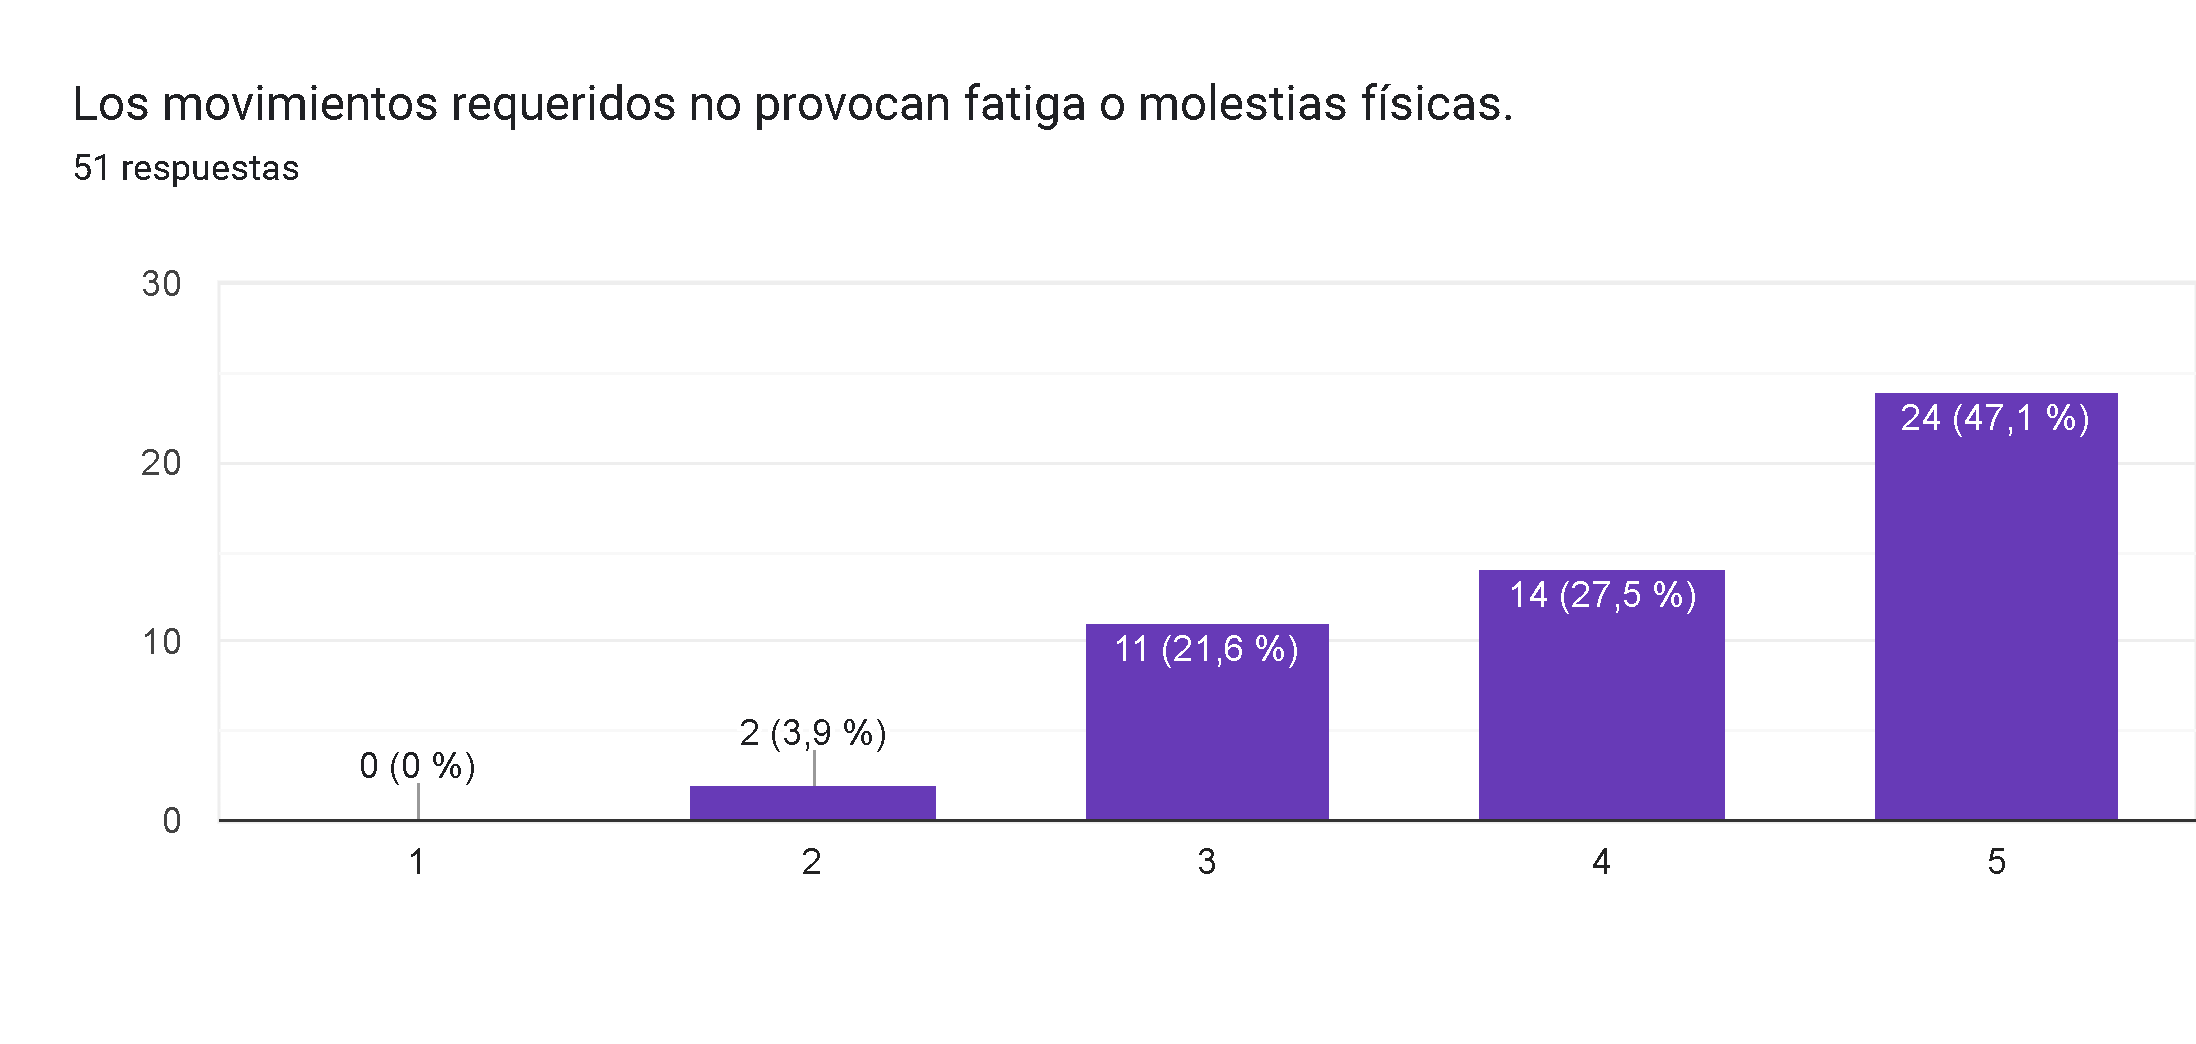
\includegraphics[width=0.7\linewidth]{Imagenes/fc5.png}
  \caption{Elaboración propia, Módulo fitness, Imagen de referencia sobre cuestionario  de gamificación para el módulo fitness del juego sobre la muñeca, ``Los movimientos requeridos no provocan fatiga o molestias físicas``}
  \label{fig:cuestionario5fitness}
\end{figure}


La pregunta ``La interfaz del usuario es clara y fácil de usar`` obtuvo la mayor cantidad de respuestas en la opción 4, con un 30,8 \%. Esto indica que la interfaz es generalmente considerada clara y fácil de usar, aunque algunos usuarios podrían sugerir mejoras para una mayor simplicidad o accesibilidad.

    \begin{figure}[H]
  \centering
  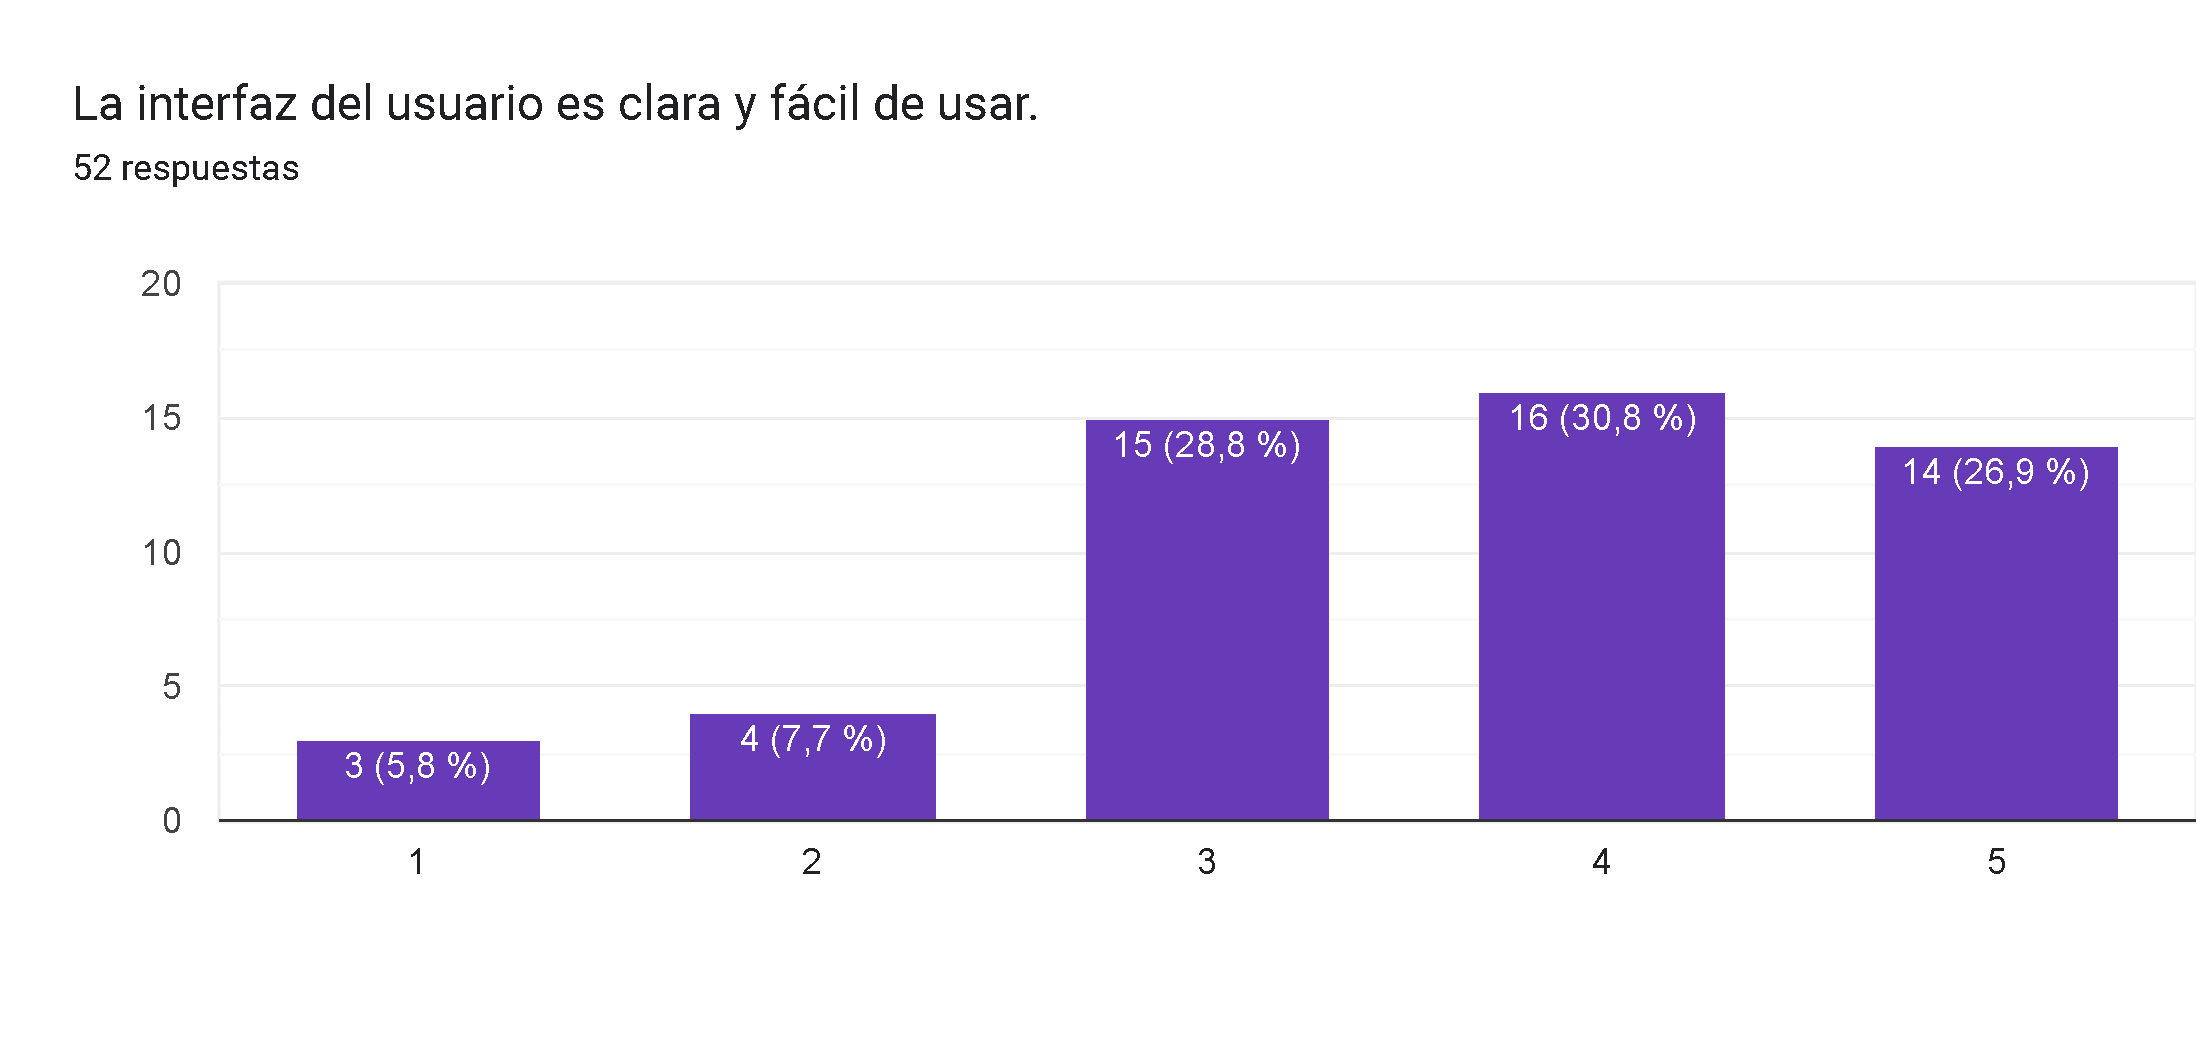
\includegraphics[width=0.7\linewidth]{Imagenes/fc6.png}
  \caption{Elaboración propia, Módulo fitness, Imagen de referencia sobre cuestionario  de gamificación para el módulo fitness del juego sobre la muñeca, ``La interfaz del usuario es clara y fácil de usar``}
  \label{fig:cuestionario6fitness}
\end{figure}


La pregunta ``El juego se ejecuta sin problemas de rendimiento (lag, caídas de FPS, etc.)`` obtuvo la mayor cantidad de respuestas en la opción 4, con un 40,4 \%. Esto sugiere que el rendimiento del juego es generalmente adecuado, aunque algunos usuarios podrían experimentar leves inconvenientes con el rendimiento.
    \begin{figure}[H]
  \centering
  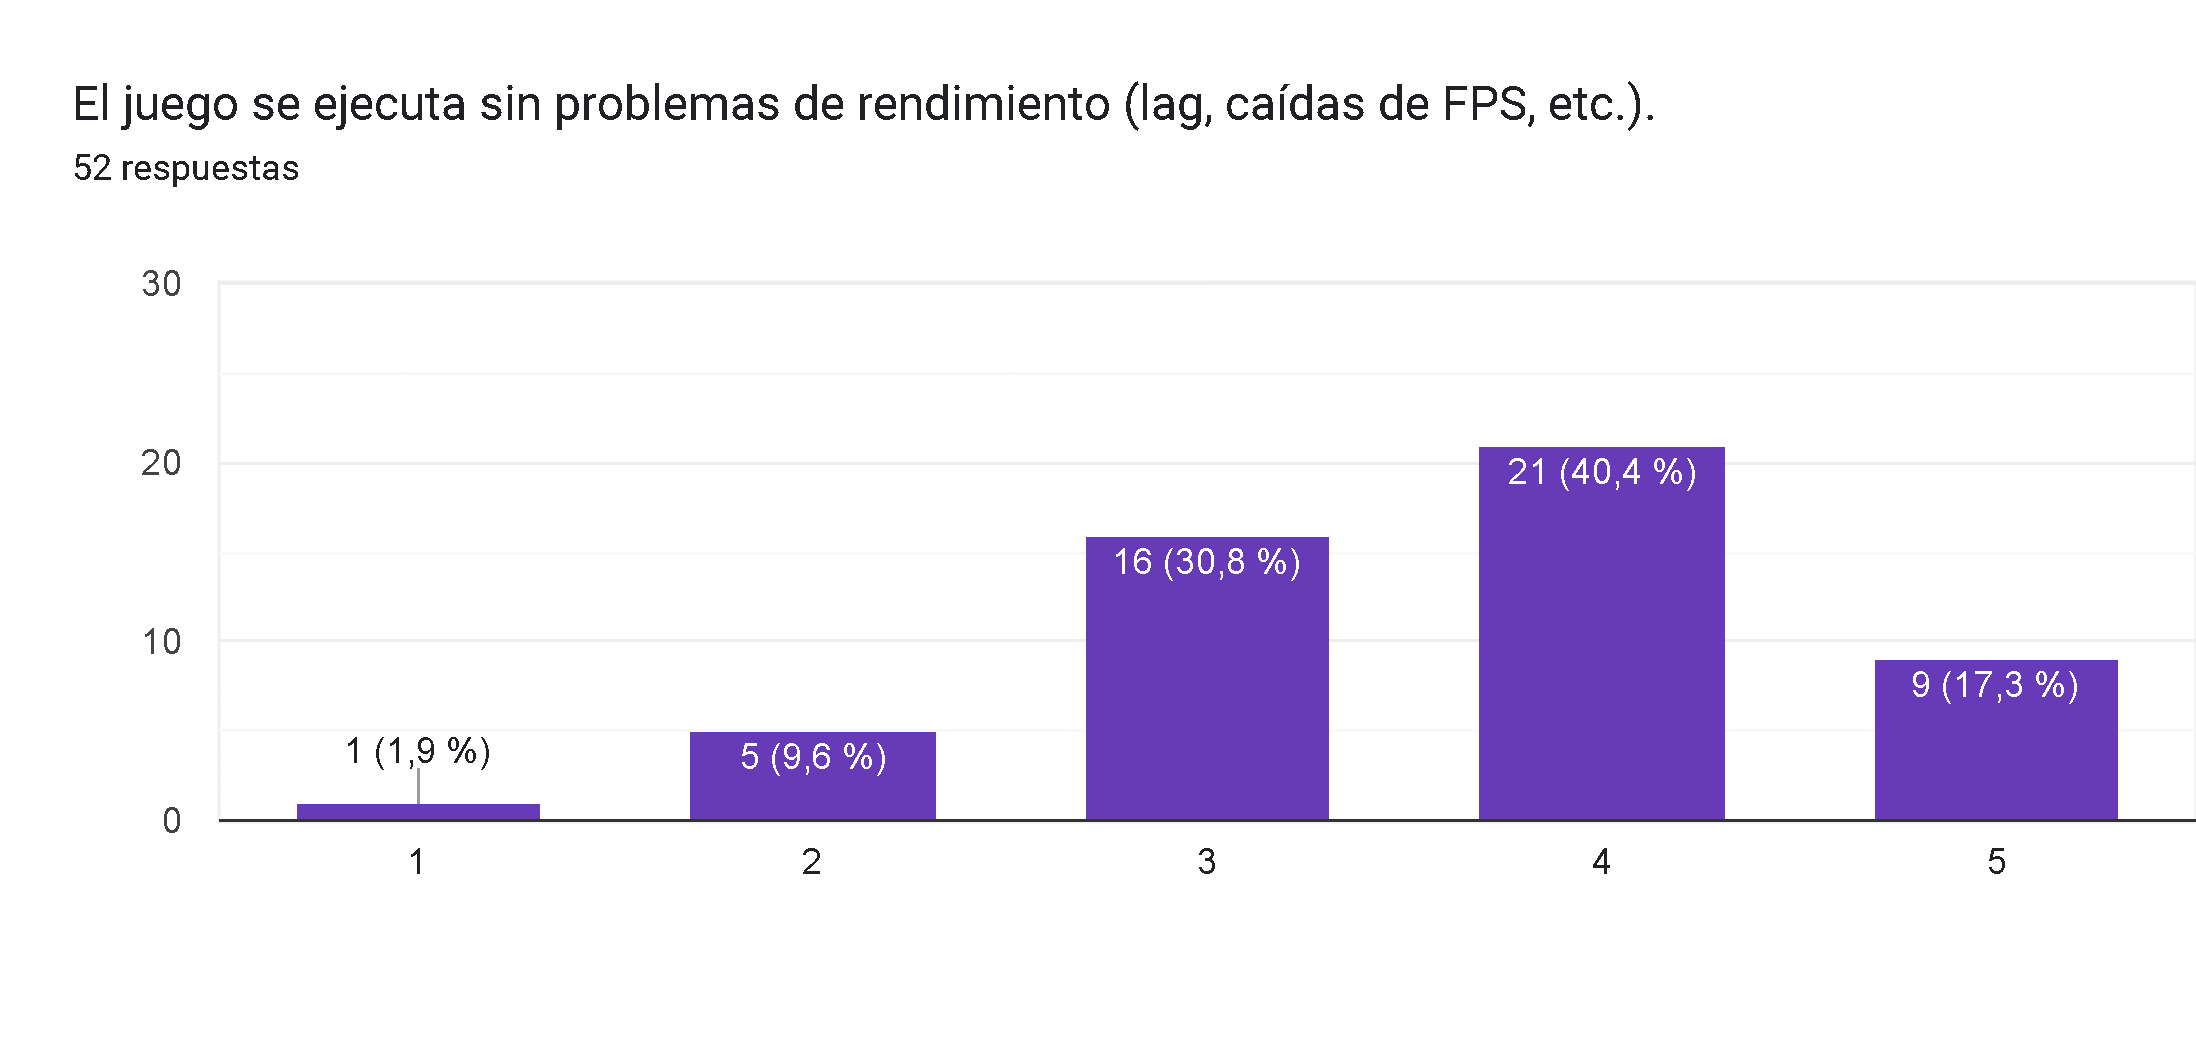
\includegraphics[width=0.7\linewidth]{Imagenes/fc7.png}
  \caption{Elaboración propia, Módulo fitness, Imagen de referencia sobre cuestionario  de gamificación para el módulo fitness del juego sobre la muñeca,``El juego se ejecuta sin problemas de rendimiento (lag, caídas de FPS, etc.)`` }
  \label{fig:cuestionario7fitness}
\end{figure}


La pregunta ``No he experimentado fallos técnicos o bugs importantes`` obtuvo la mayor cantidad de respuestas en la opción 4, con un 51,9 \%. Esto indica que la mayoría de los usuarios no han experimentado problemas técnicos significativos, aunque un porcentaje menor aún podría haber encontrado algunos inconvenientes.

    \begin{figure}[H]
  \centering
  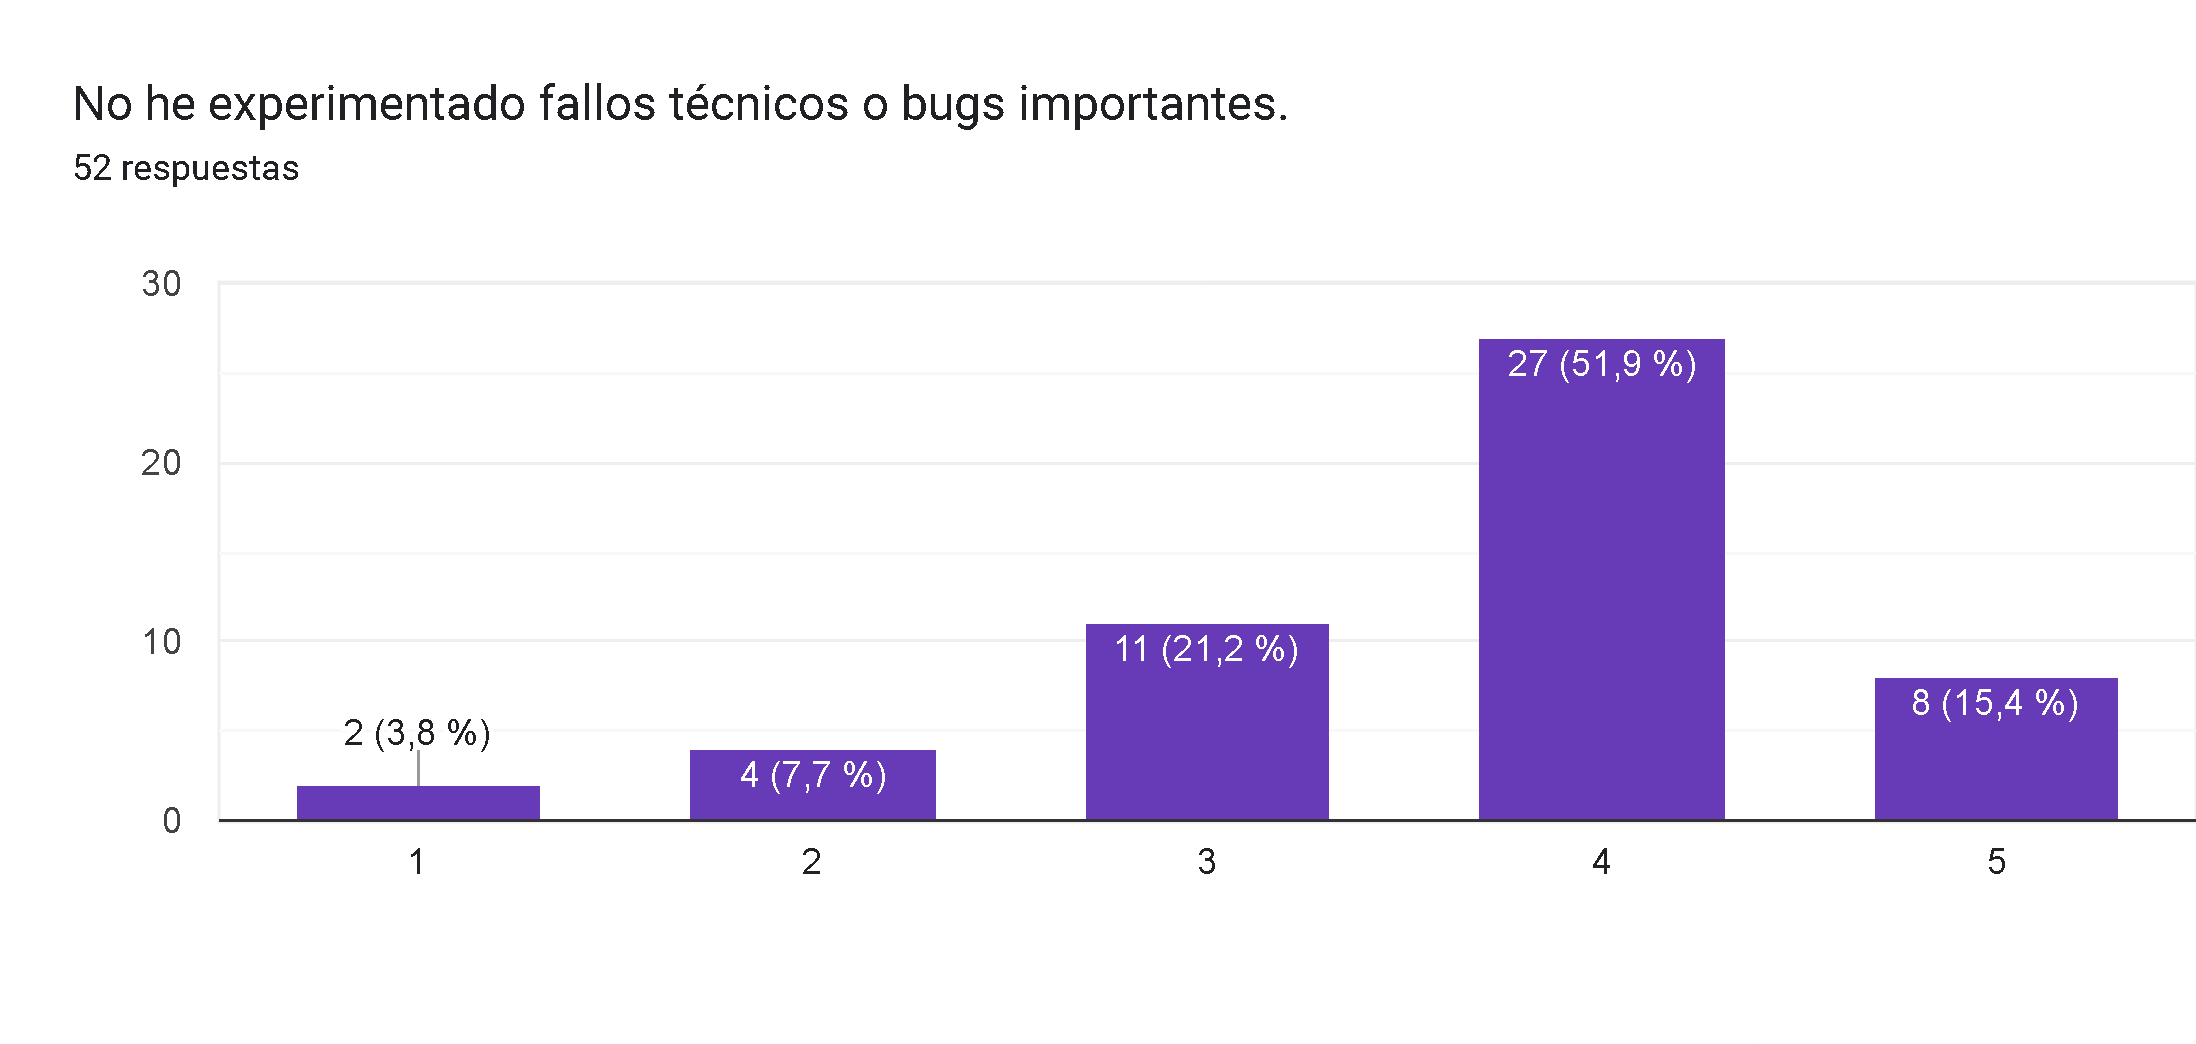
\includegraphics[width=0.7\linewidth]{Imagenes/fc8.png}
  \caption{Elaboración propia, Módulo fitness, Imagen de referencia sobre cuestionario  de gamificación para el módulo fitness del juego sobre la muñeca,``No he experimentado fallos técnicos o bugs importantes``}
  \label{fig:cuestionario8fitness}
\end{figure}

La pregunta ``El juego me ha mantenido motivado para seguir jugando`` obtuvo la misma cantidad de respuestas en las opciones 4 y 3, con un 30,8 \% en ambas. Esto sugiere que la motivación del jugador varía, con una parte significativa encontrando el juego suficientemente motivador, mientras que otros podrían necesitar más incentivos para seguir jugando.

    \begin{figure}[H]
  \centering
  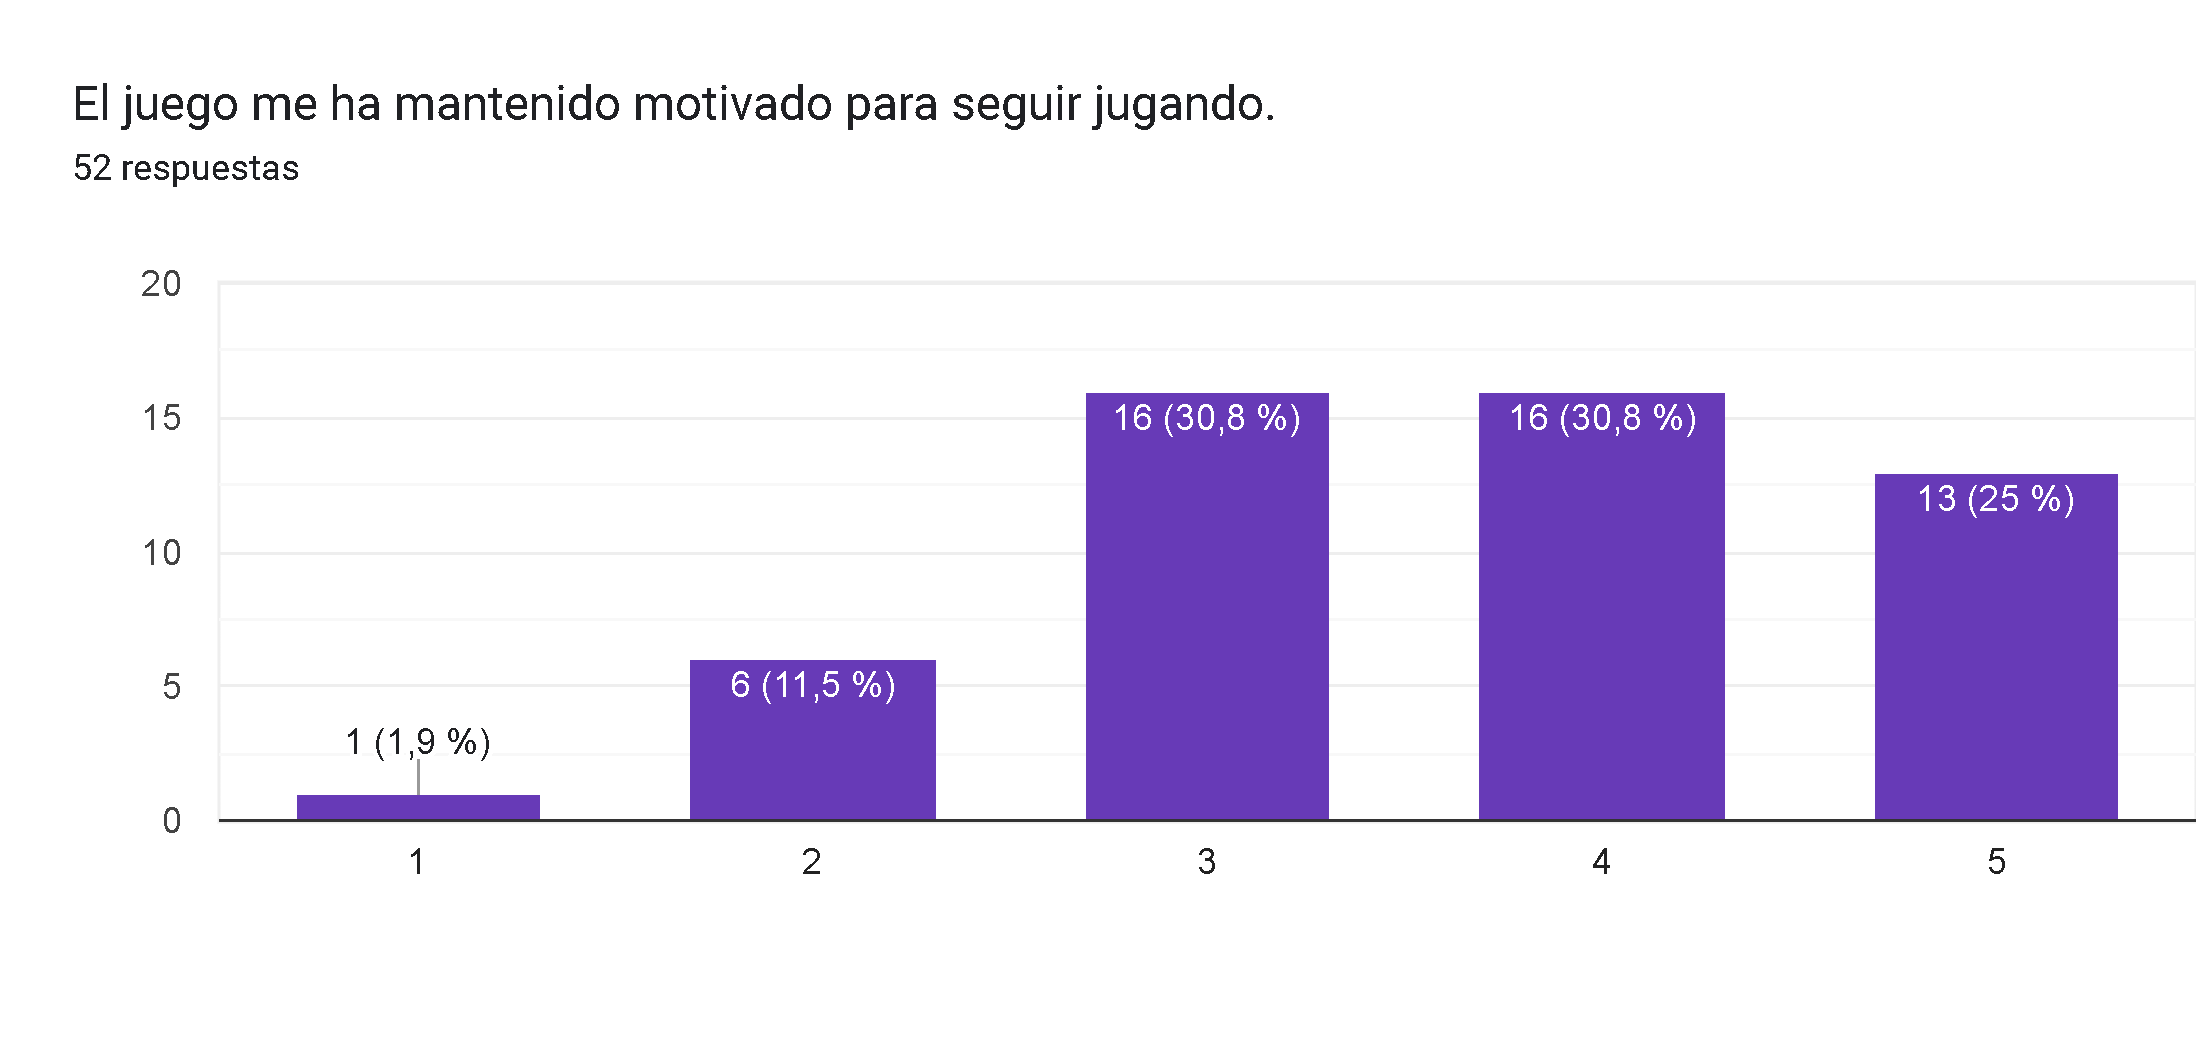
\includegraphics[width=0.7\linewidth]{Imagenes/fc9.png}
  \caption{Elaboración propia, Módulo fitness, Imagen de referencia sobre cuestionario  de gamificación para el módulo fitness del juego sobre la muñeca,``El juego me ha mantenido motivado para seguir jugando`` }
  \label{fig:cuestionario9fitness}
\end{figure}


La pregunta ``Me siento satisfecho con la experiencia general del juego`` obtuvo la mayor cantidad de respuestas en la opción 4, con un 44,2 \%. Esto sugiere que la mayoría de los usuarios están satisfechos con la experiencia general, aunque algunos todavía pueden encontrar áreas para mejorar.

    \begin{figure}[H]
  \centering
  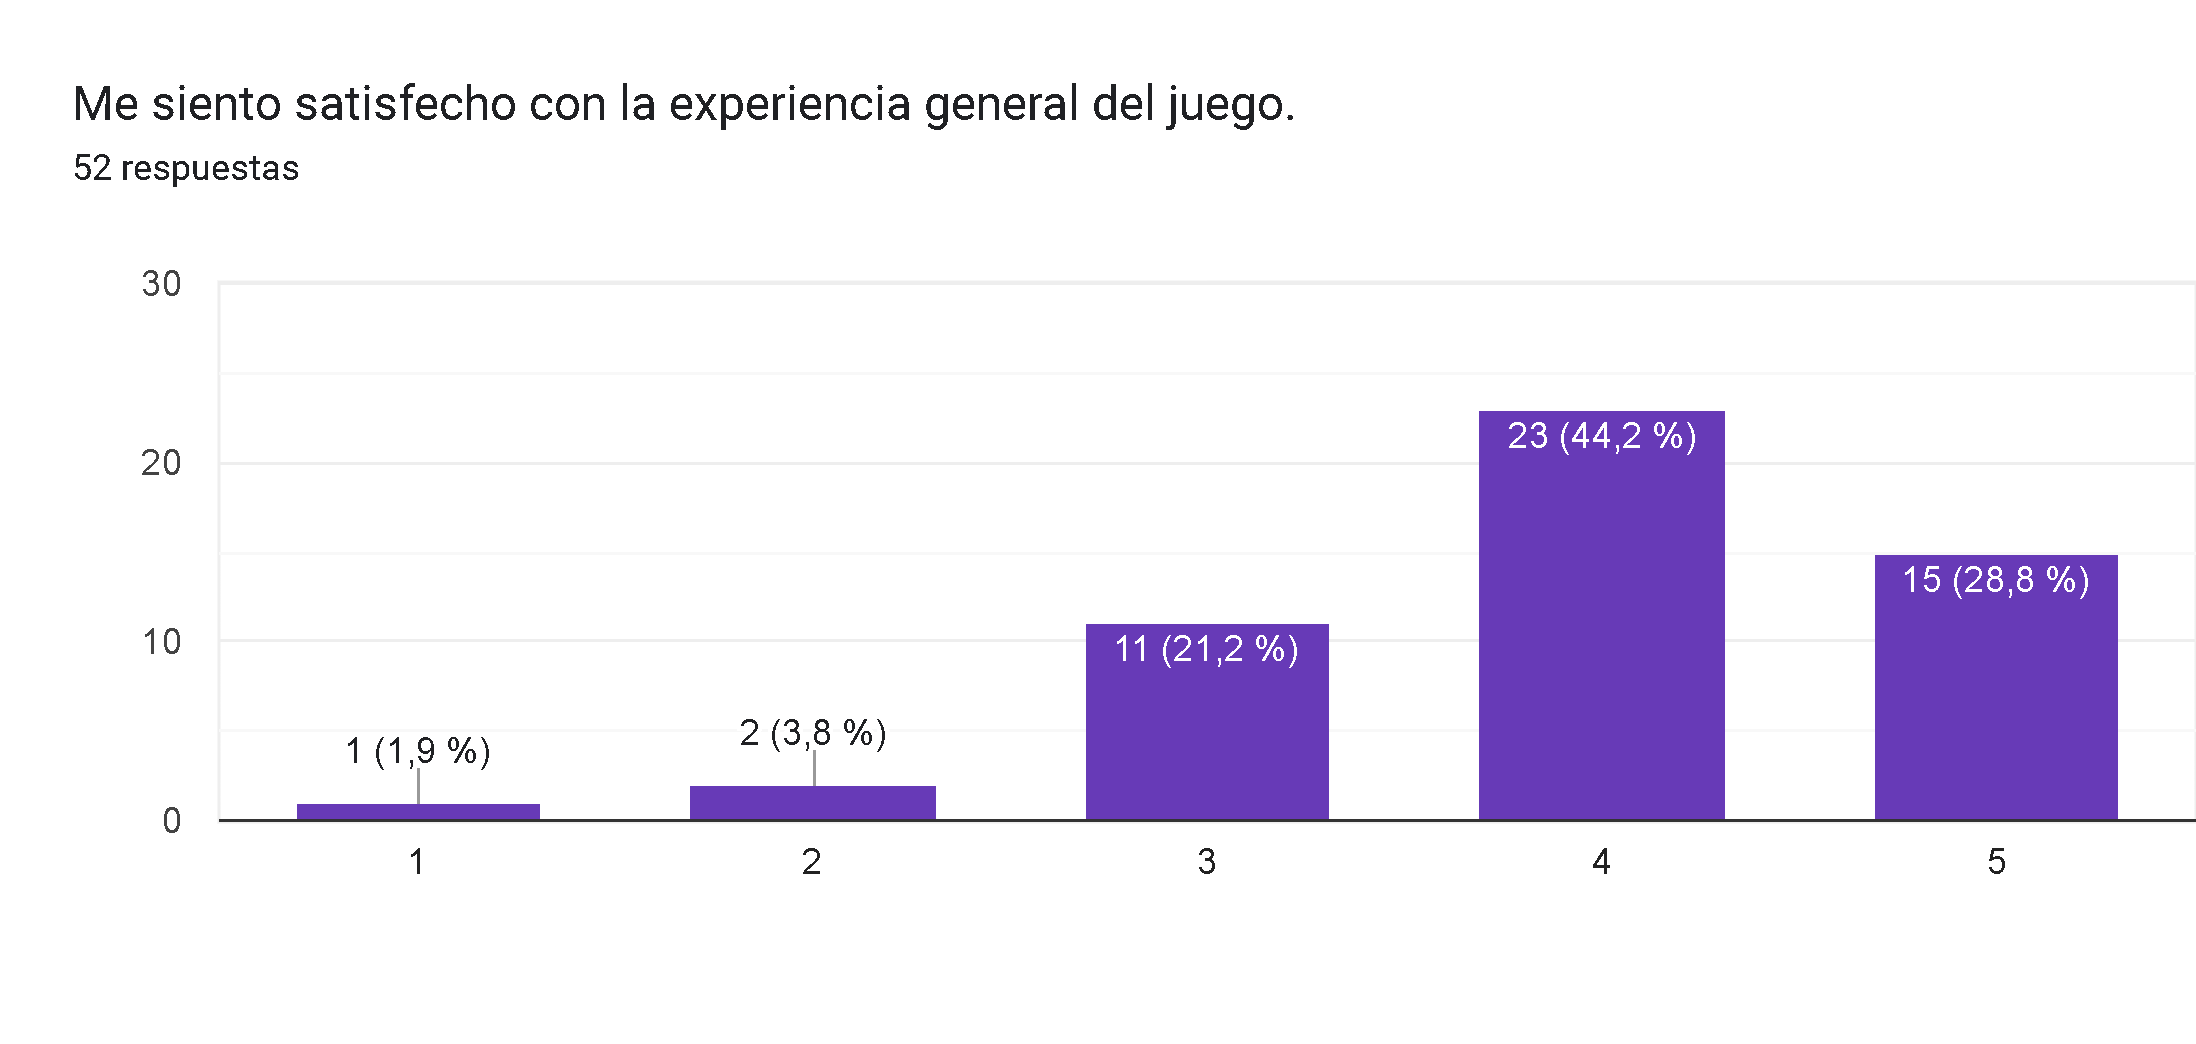
\includegraphics[width=0.7\linewidth]{Imagenes/fc10.png}
  \caption{Elaboración propia, Módulo fitness, Imagen de referencia sobre cuestionario  de gamificación para el módulo fitness del juego sobre la muñeca,``Me siento satisfecho con la experiencia general del juego``}
  \label{fig:cuestionario10fitness}
\end{figure}

La pregunta ``Consideras que el juego es útil para ayudar a la prevención del túnel carpiano`` obtuvo la mayor cantidad de respuestas en la opción 4, con un 38,5 \%. Además, un 19,2 \% eligió la opción 3, lo que indica que una parte significativa de los usuarios considera que el juego puede ser útil para la prevención del túnel carpiano, aunque una proporción considerable aún no está completamente segura de su efectividad.


    \begin{figure}[H]
  \centering
  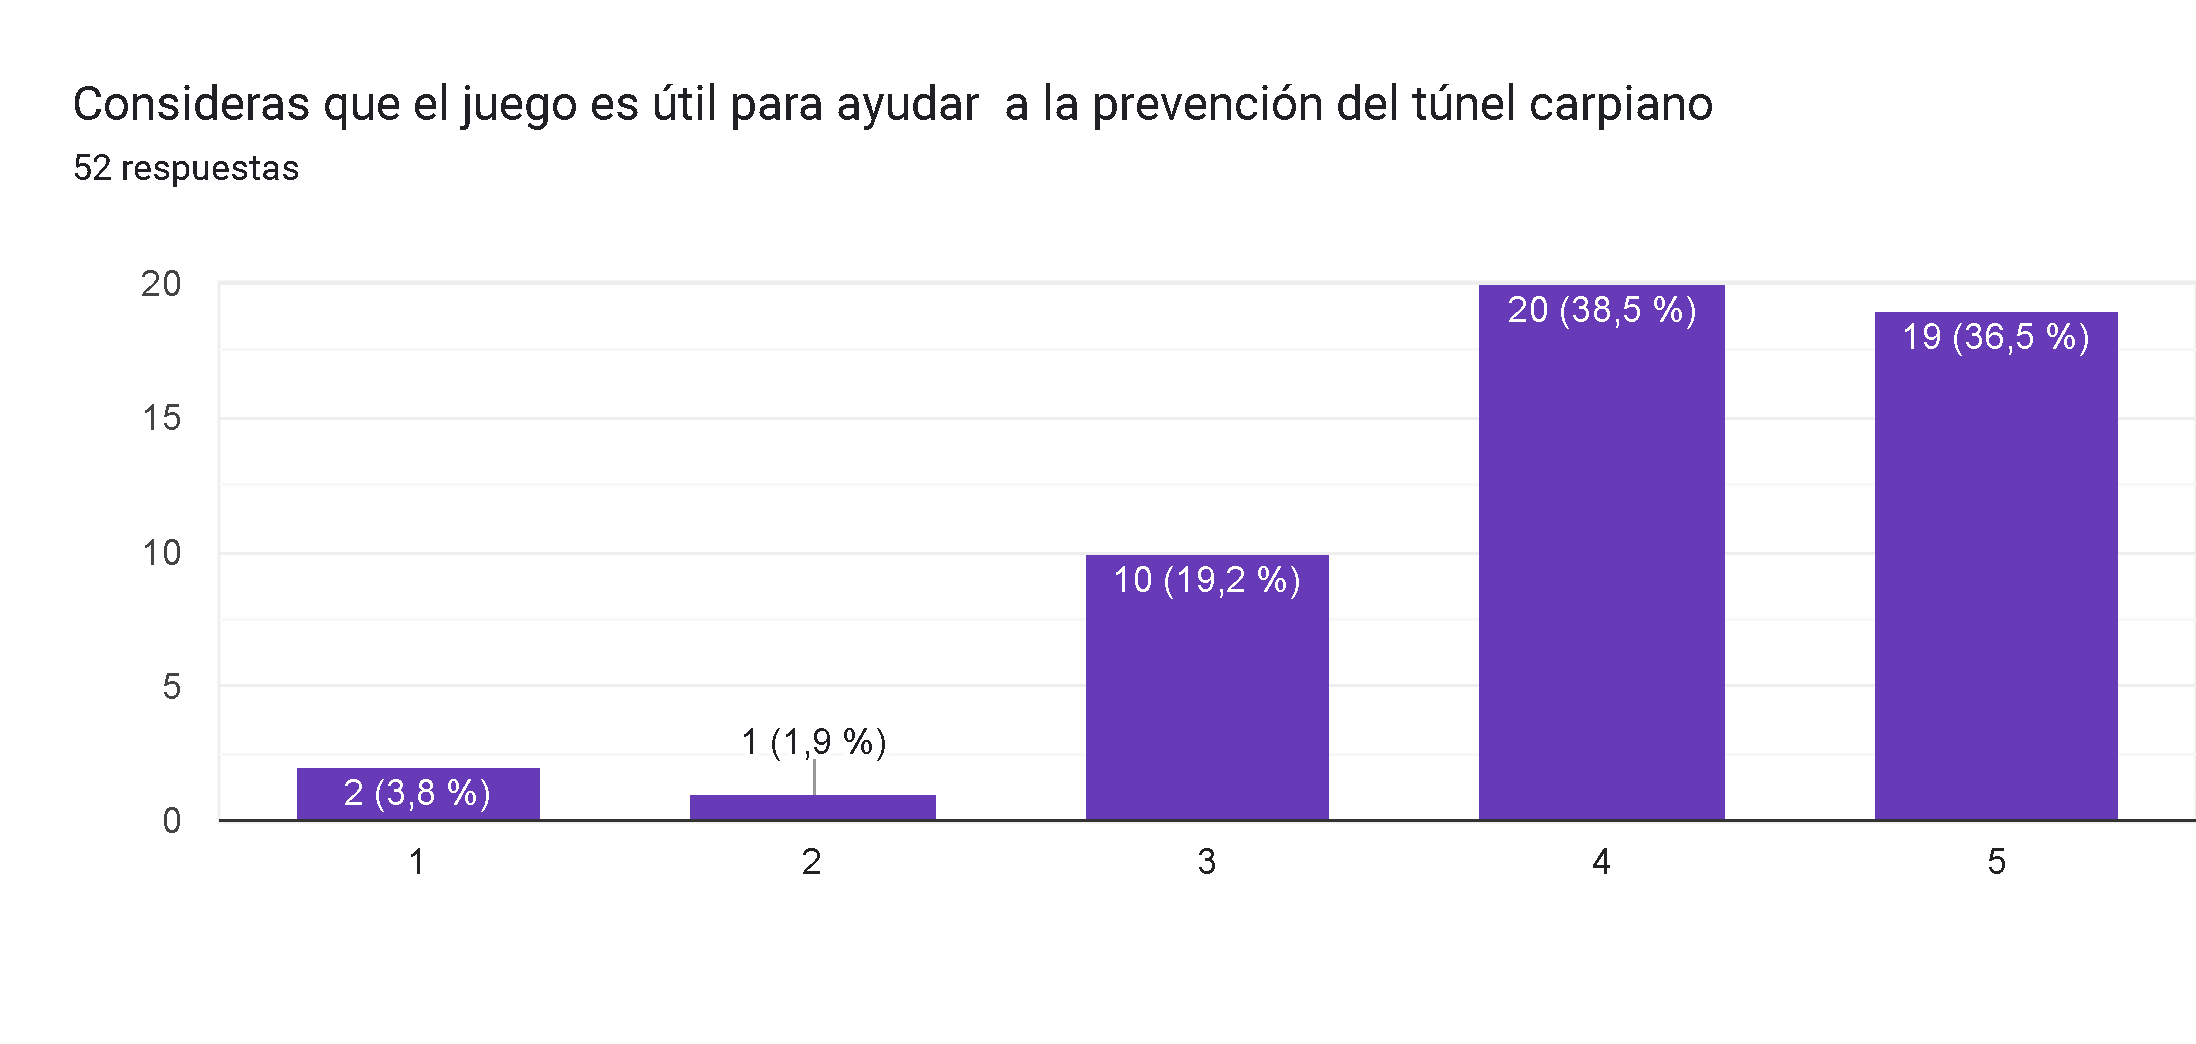
\includegraphics[width=0.7\linewidth]{Imagenes/fc11.png}
  \caption{Elaboración propia, Módulo fitness, Imagen de referencia sobre cuestionario  de gamificación para el módulo fitness del juego sobre la muñeca,``Consideras que el juego es útil para ayudar a la prevención del túnel carpiano``  }
  \label{fig:cuestionario11fitness}
\end{figure}



\subsection{Fitness: Juego sobre movimiento de la espalda}
La pregunta ``El juego es fácil de entender y aprender`` obtuvo la mayor cantidad de respuestas en la opción 4, con un 41,2 \%. Esto indica que la mayoría de los usuarios consideran que el juego es comprensible y fácil de aprender, aunque una parte también encuentra áreas que podrían mejorarse para facilitar aún más su comprensión.

\begin{figure}[H]
  \centering
  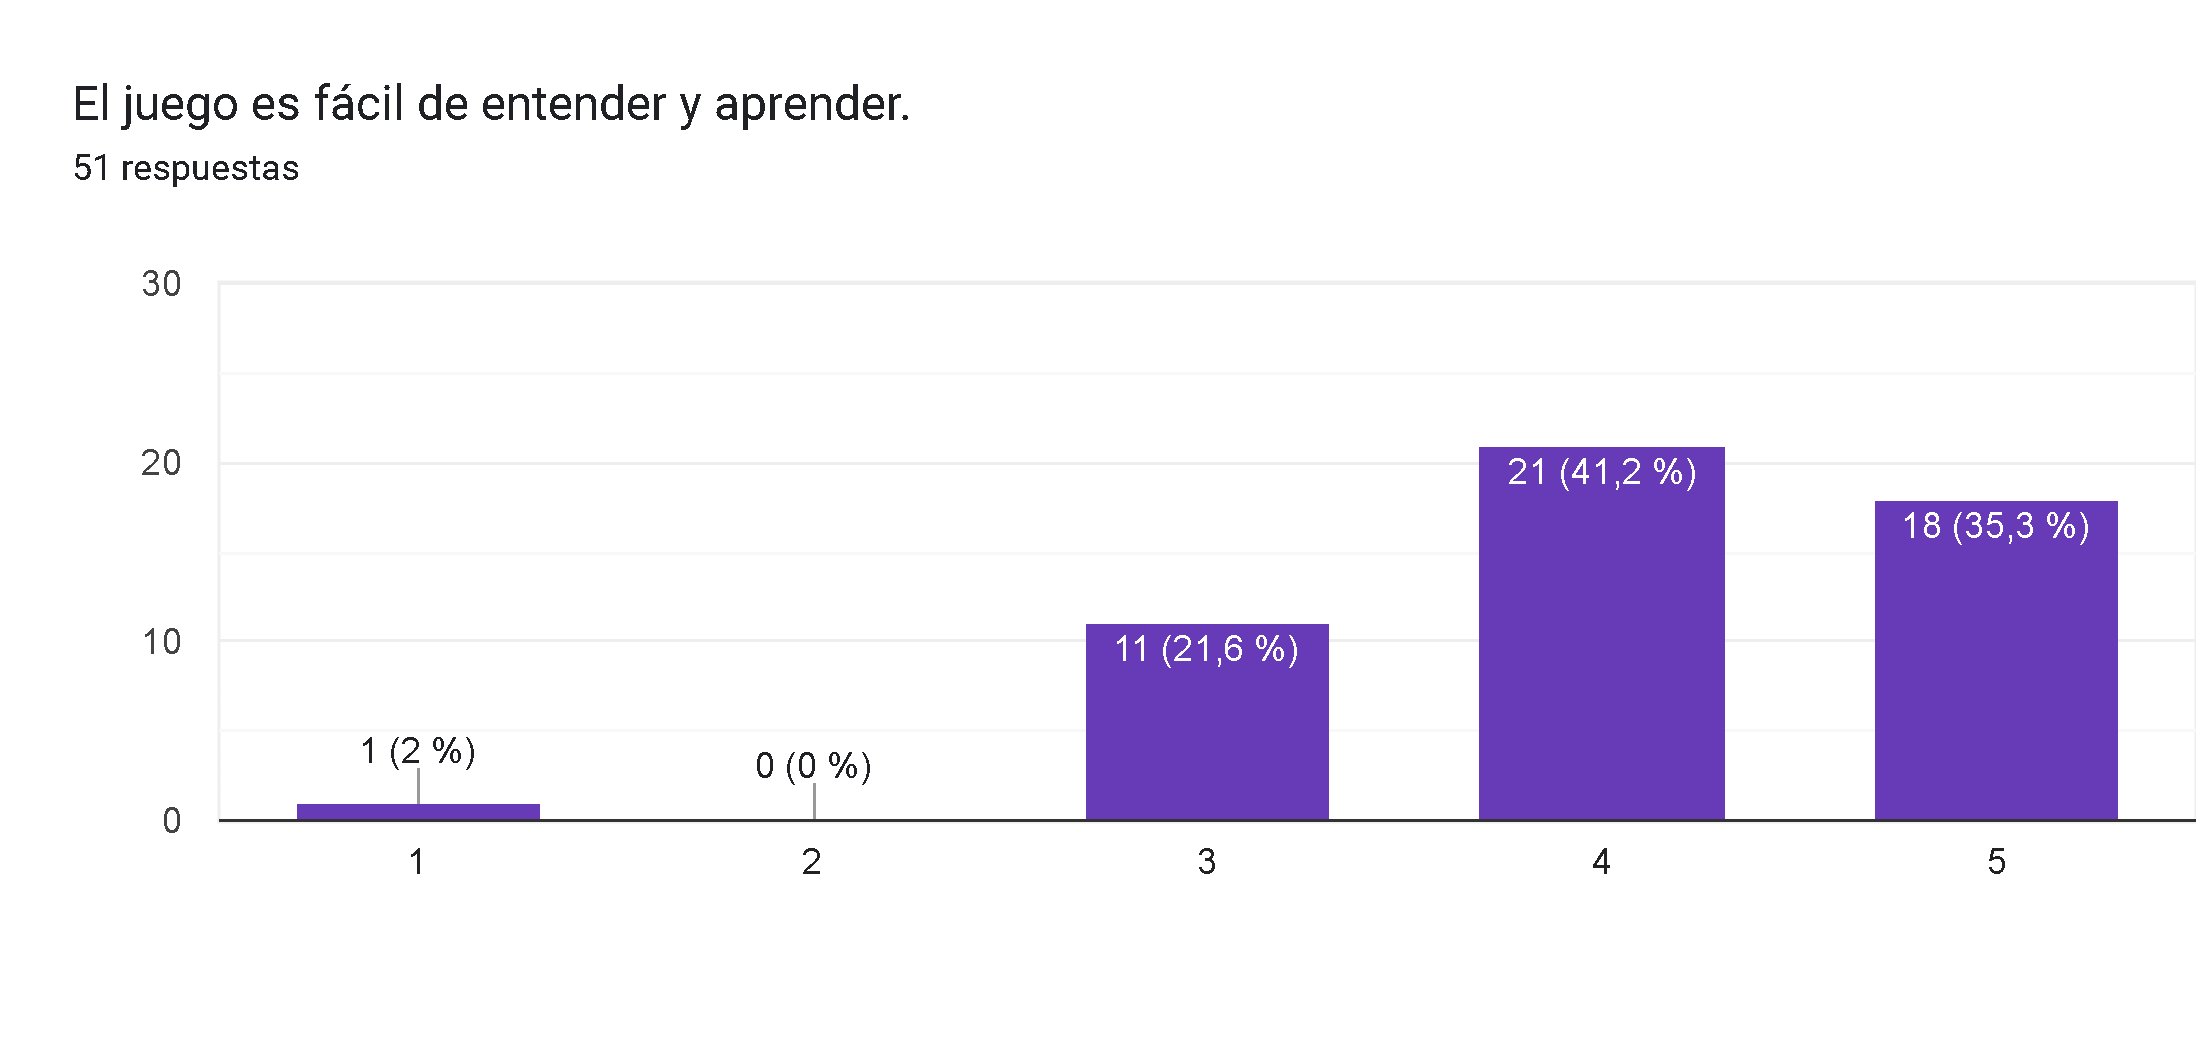
\includegraphics[width=0.7\linewidth]{Imagenes/fd1.png}
  \caption{Elaboración propia, Módulo fitness, Imagen de referencia sobre cuestionario de gamificación para el módulo fitness del juego sobre el movimiento de la espalda, ``El juego es fácil de entender y aprender``}
  \label{fig:cuestionario12fitness}
\end{figure}


La pregunta ``Los controles son intuitivos y responden bien`` obtuvo 24 respuestas en la opción 4, con una mayoría de opiniones positivas. Esto sugiere que los sensores para indicar la posición de la espalda funcionan de manera adecuada, brindando una experiencia satisfactoria a los usuarios.

\begin{figure}[H]
  \centering
  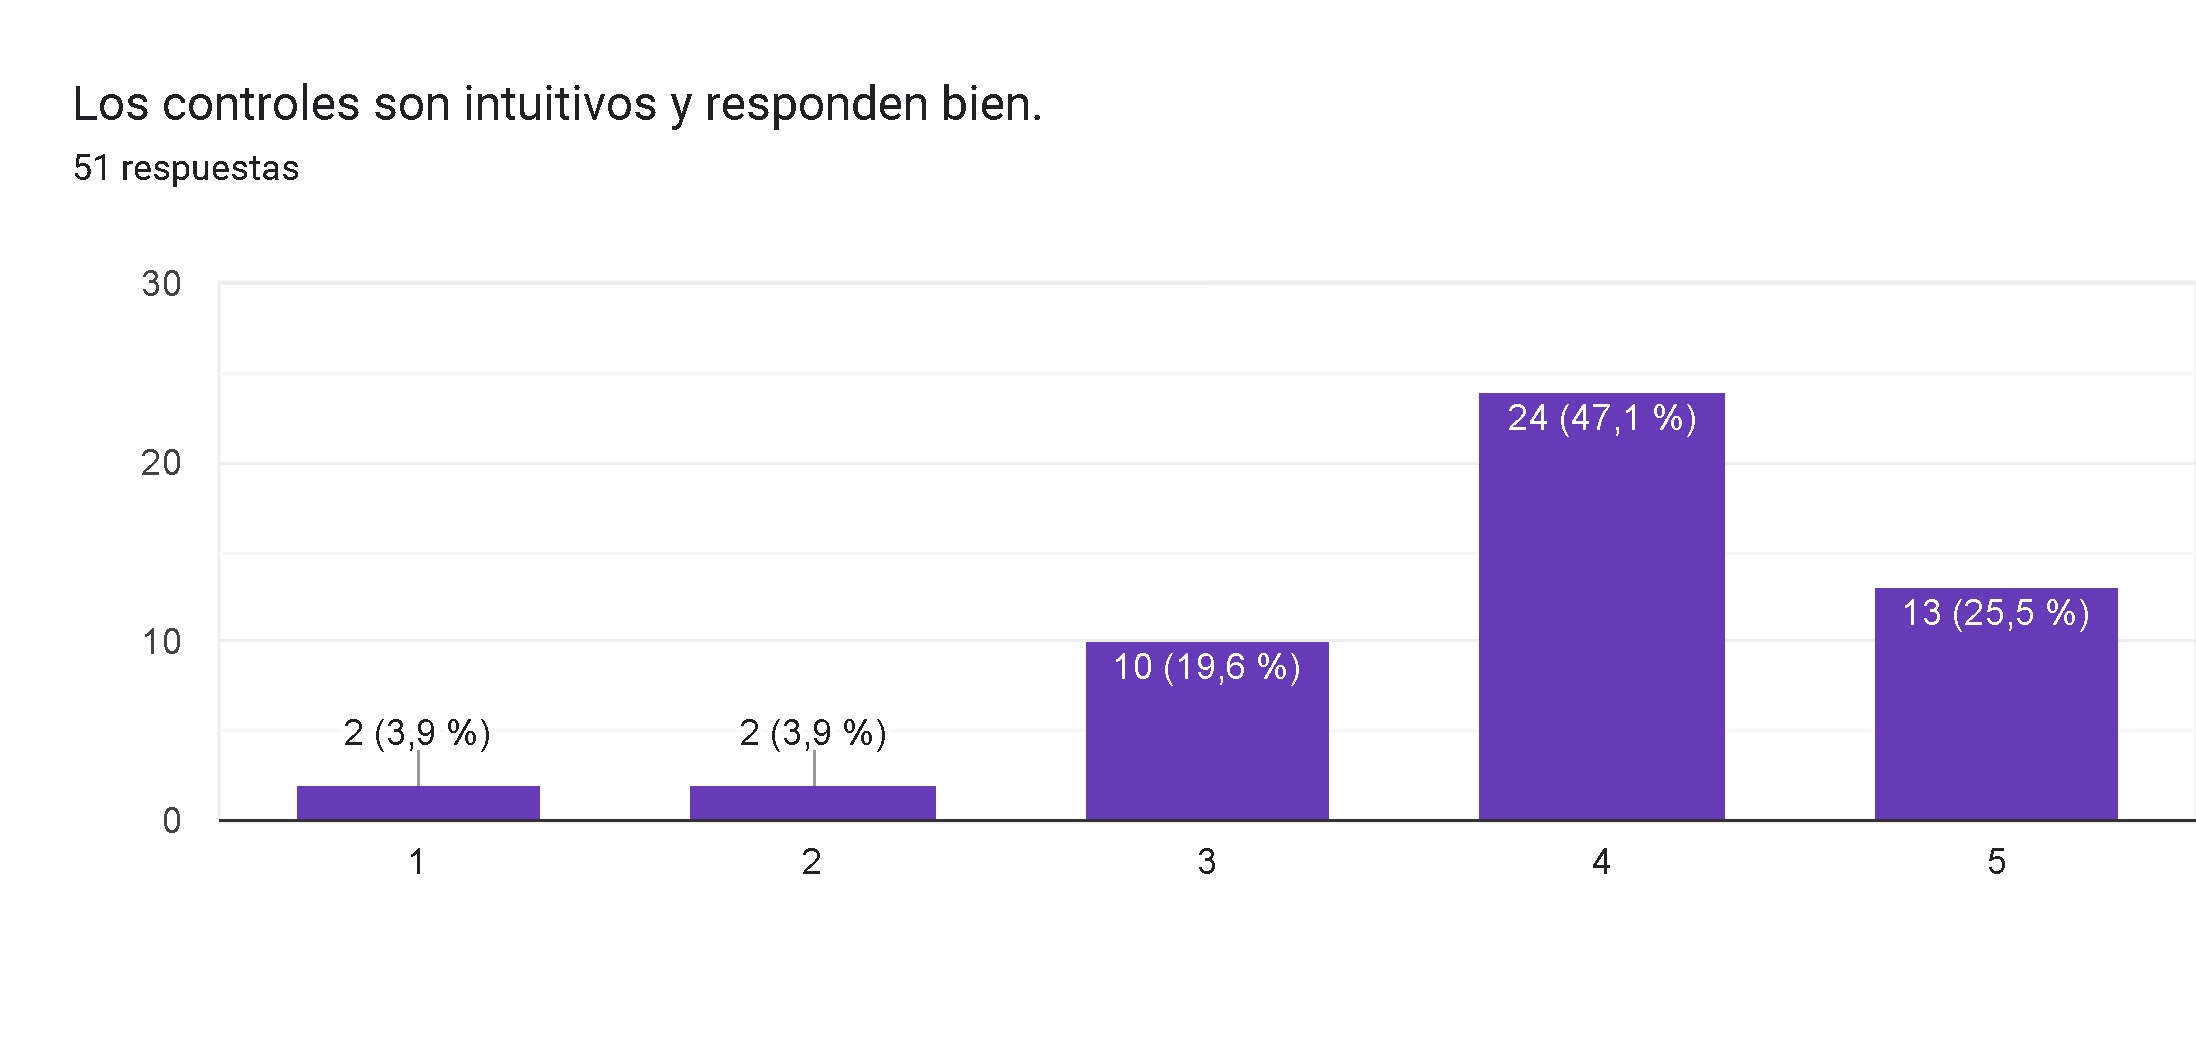
\includegraphics[width=0.7\linewidth]{Imagenes/fd2.png}
  \caption{Elaboración propia, Módulo fitness, Imagen de referencia sobre cuestionario de gamificación para el módulo fitness del juego sobre el movimiento de la espalda, ``Los controles son intuitivos y responden bien``}
  \label{fig:cuestionario13fitness}
\end{figure}

La pregunta ``El nivel de dificultad es adecuado`` obtuvo la mayor cantidad de respuestas en la opción 4, con un 44,9 \%. Esto sugiere que la mayoría de los usuarios consideran que el nivel de dificultad está bien equilibrado, aunque algunos aún podrían encontrarlo demasiado fácil o desafiante.

\begin{figure}[H]
  \centering
  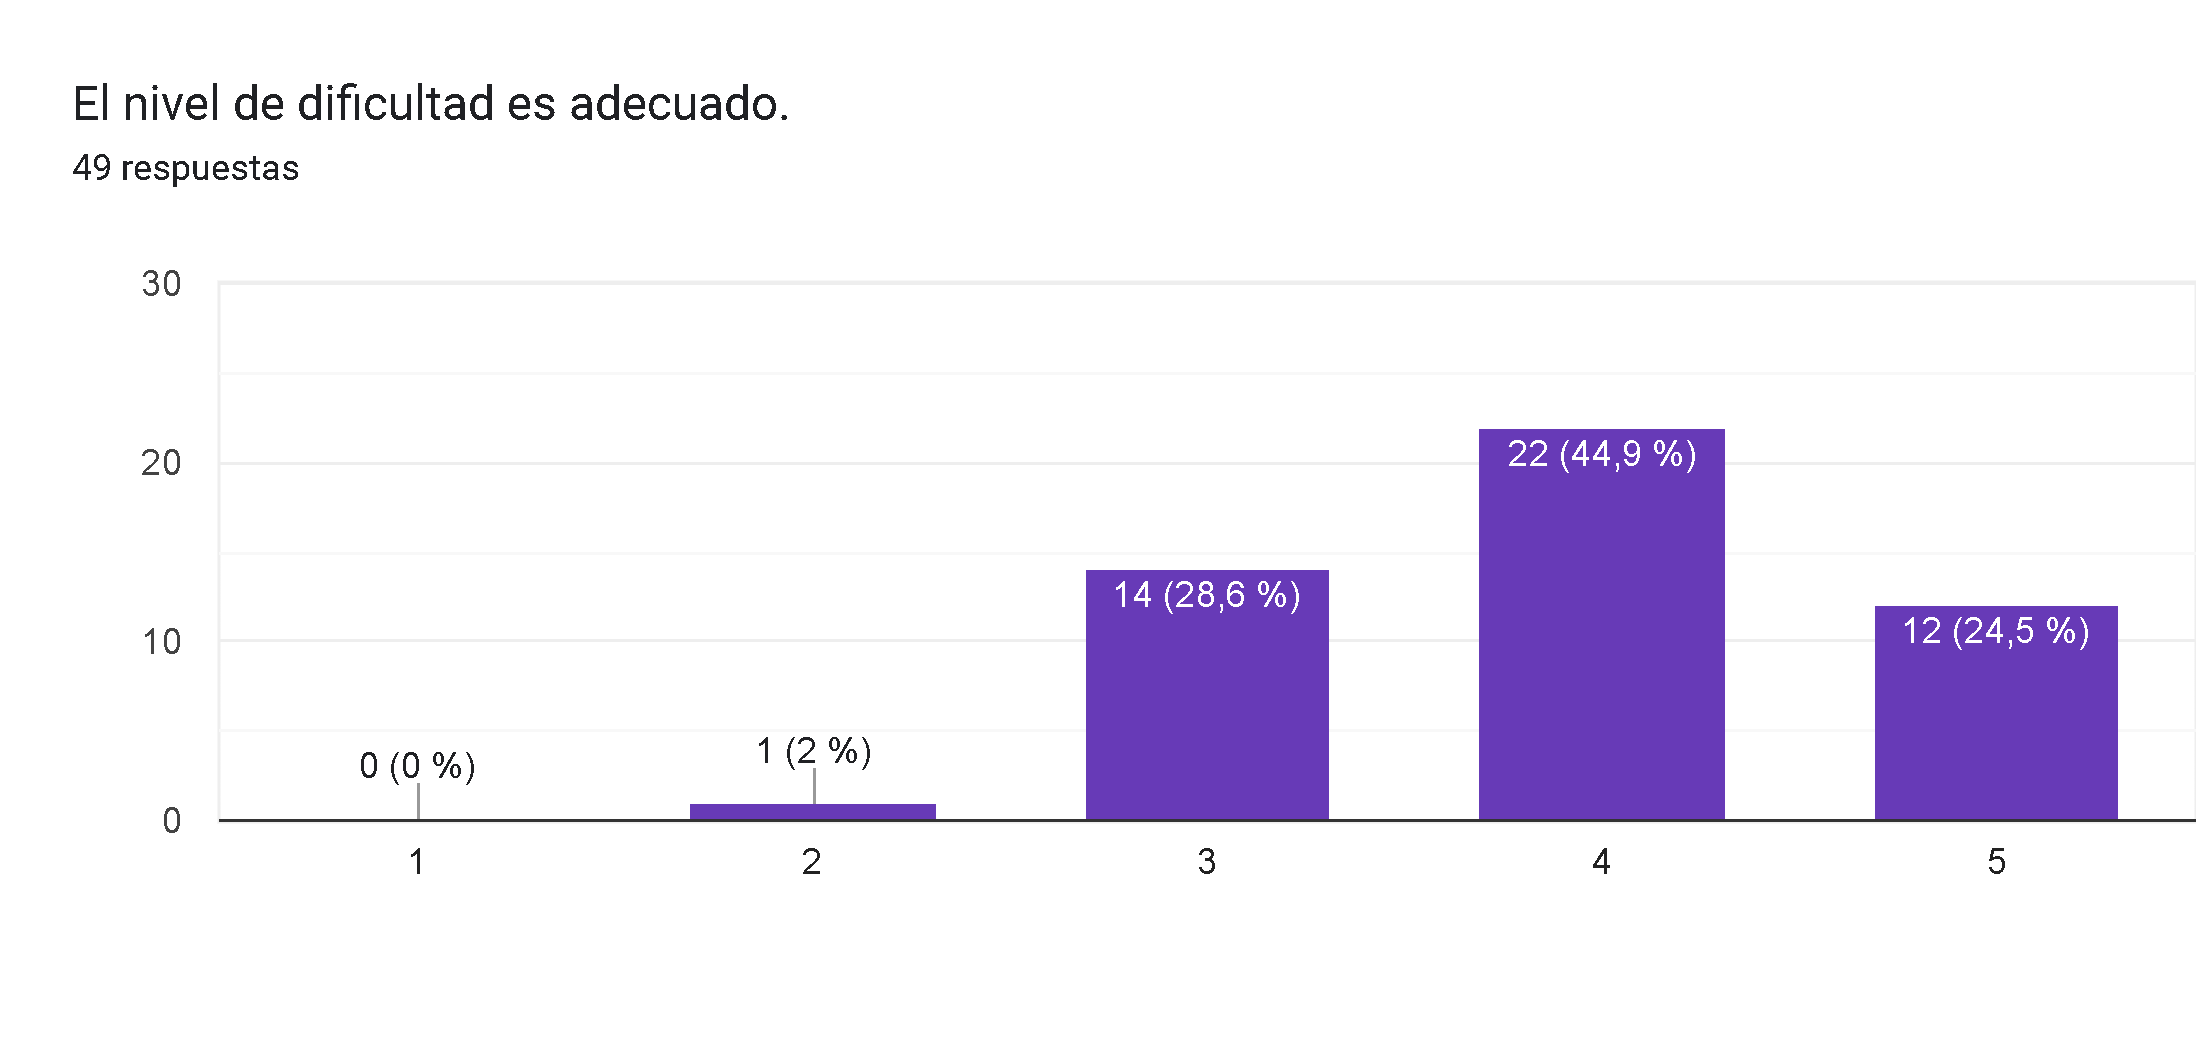
\includegraphics[width=0.7\linewidth]{Imagenes/fd3.png}
  \caption{Elaboración propia, Módulo fitness, Imagen de referencia sobre cuestionario de gamificación para el módulo fitness del juego sobre el movimiento de la espalda, ``El nivel de dificultad es adecuado``}
  \label{fig:cuestionario14fitness}
\end{figure}


La pregunta ``El juego detecta mis movimientos corporales de manera precisa`` obtuvo la mayor cantidad de respuestas en la opción 4, con un 54 \%. Sin embargo, también se observó un 22 \% de respuestas en la opción 3, lo que sugiere que, aunque la mayoría considera que la detección es precisa, hay un porcentaje significativo de usuarios que podrían experimentar dificultades o inconsistencias en la detección.

\begin{figure}[H]
  \centering
  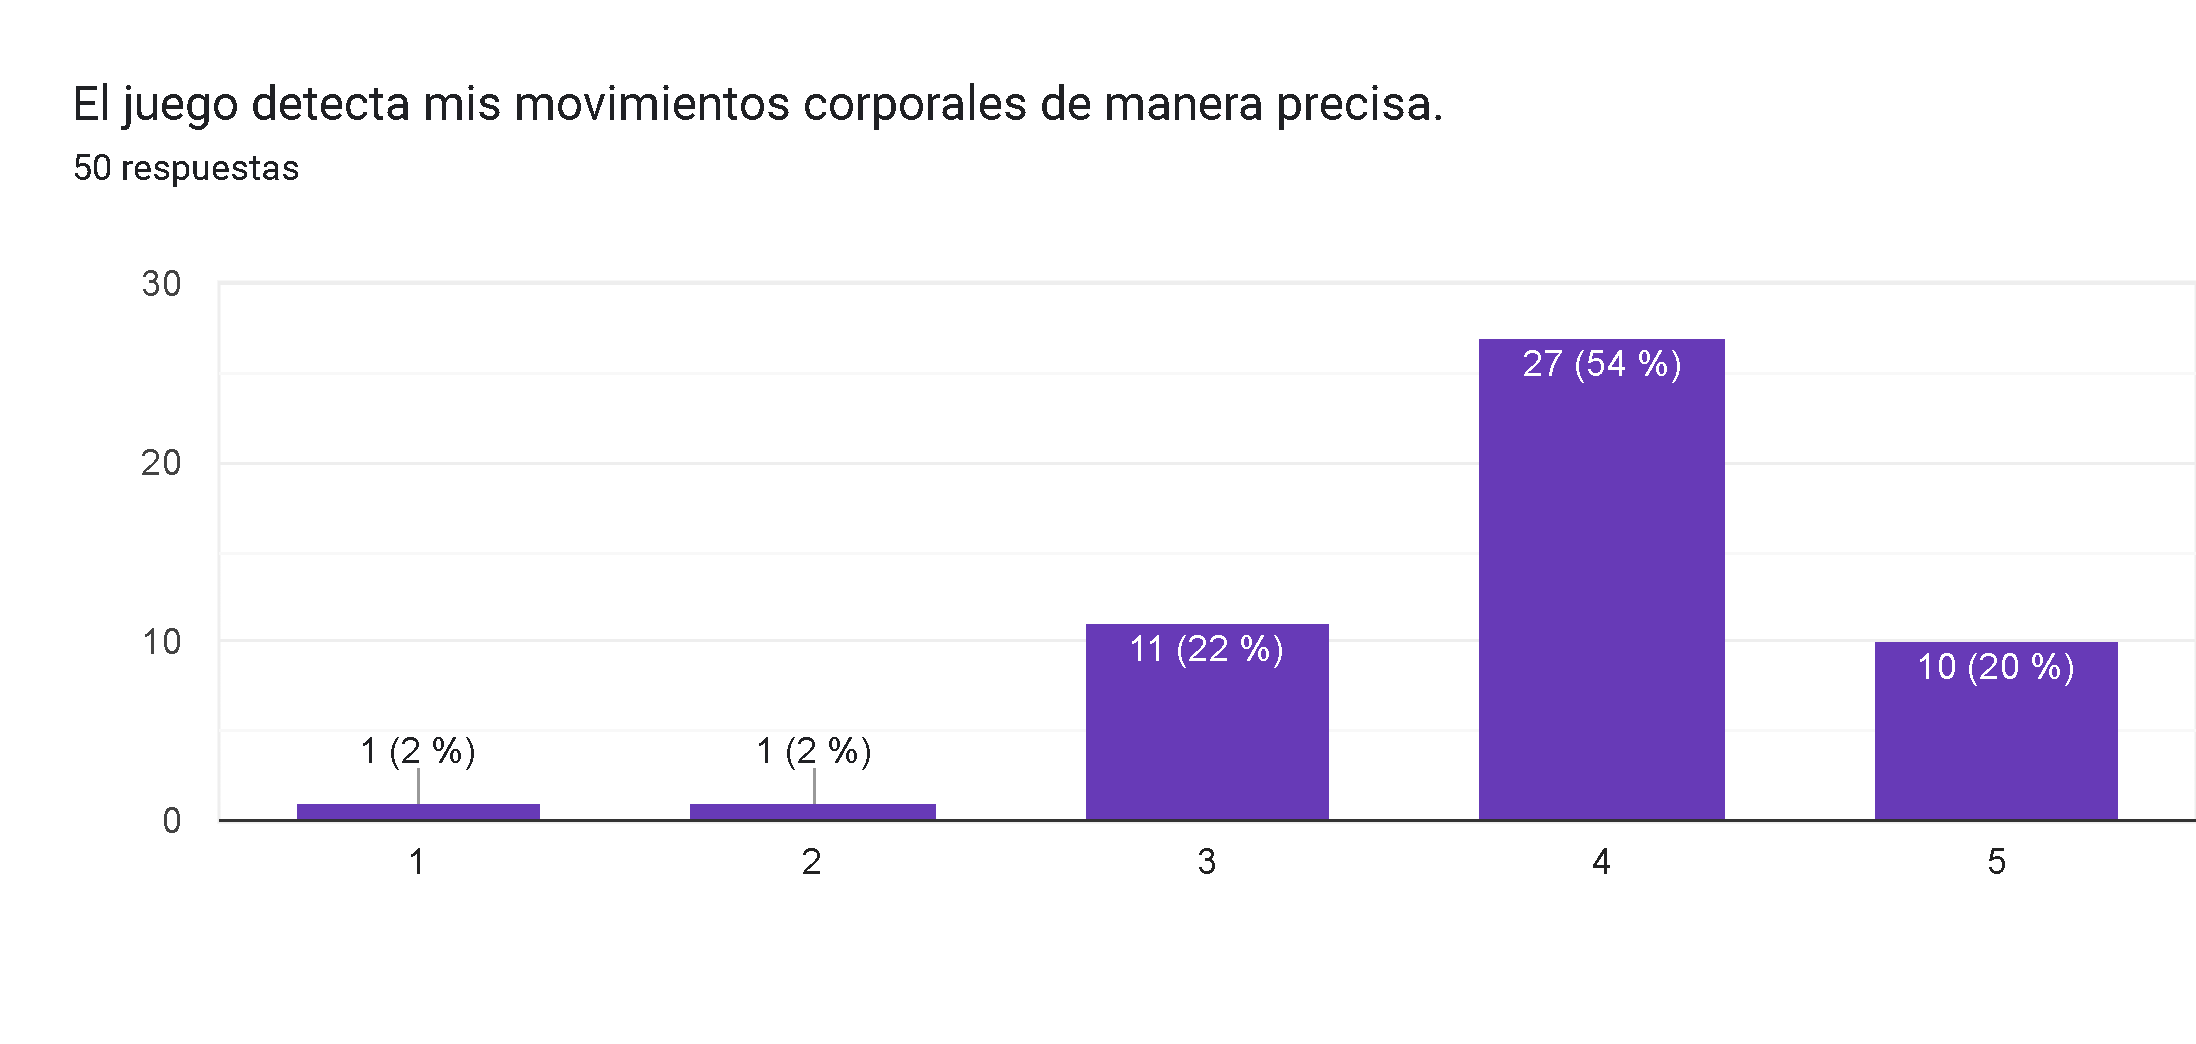
\includegraphics[width=0.7\linewidth]{Imagenes/fd4.png}
  \caption{Elaboración propia, Módulo fitness, Imagen de referencia sobre cuestionario de gamificación para el módulo fitness del juego sobre el movimiento de la espalda, ``El juego detecta mis movimientos corporales de manera precisa``}
  \label{fig:cuestionario15fitness}
\end{figure}

La pregunta ``Los movimientos requeridos no provocan fatiga o molestias físicas`` tuvo una buena recepción, con 22 respuestas en la opción 4. Esto indica que, aparentemente, los movimientos fueron cómodos para los usuarios y no generaron un ambiente incómodo para ellos.

\begin{figure}[H]
  \centering
  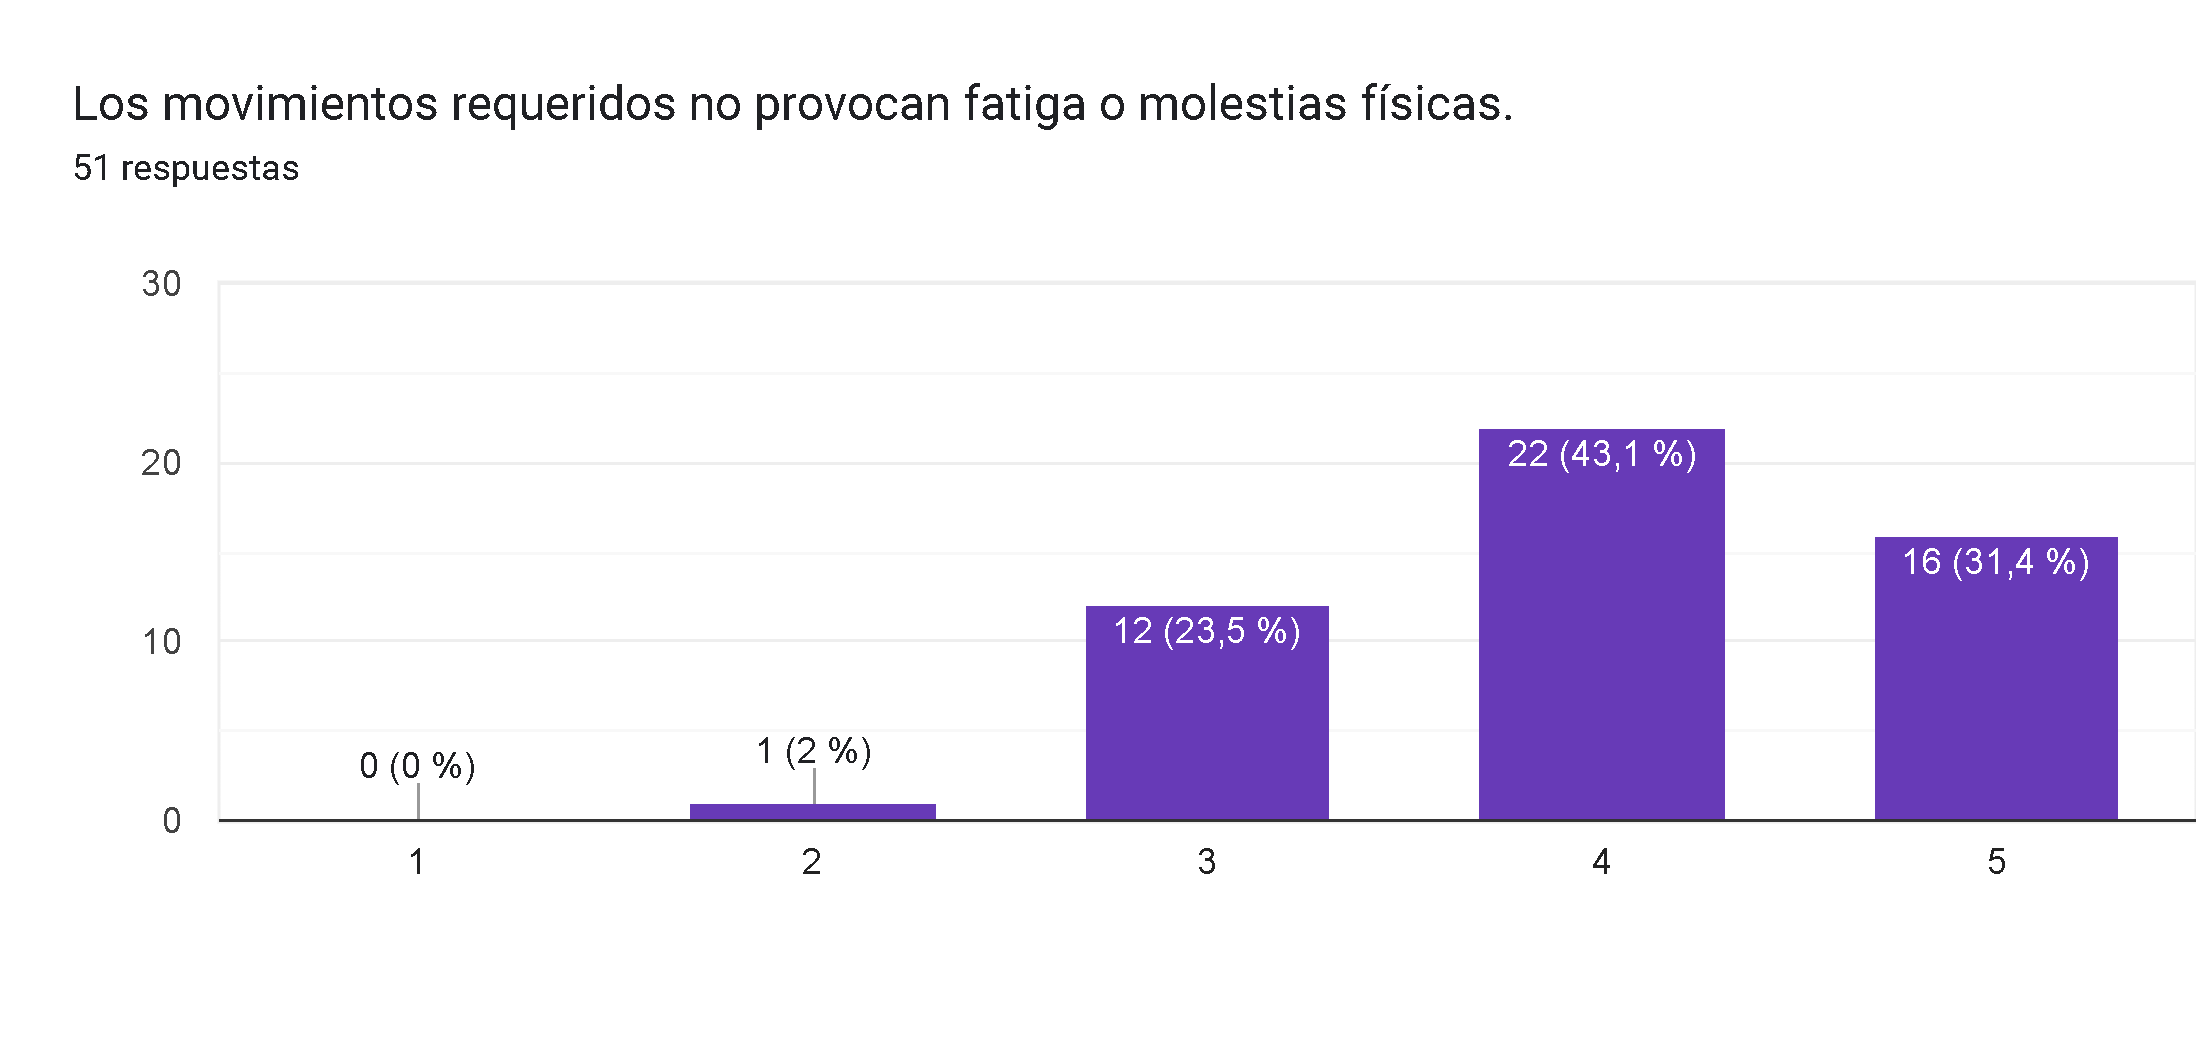
\includegraphics[width=0.7\linewidth]{Imagenes/fd5.png}
  \caption{Elaboración propia, Módulo fitness, Imagen de referencia sobre cuestionario de gamificación para el módulo fitness del juego sobre el movimiento de la espalda, ``Los movimientos requeridos no provocan fatiga o molestias físicas``}
  \label{fig:cuestionario16fitness}
\end{figure}


La pregunta ``La interfaz del usuario es clara y fácil de usar`` obtuvo la mayor cantidad de respuestas en la opción 4, con un 39,2 \%. Además, un 23,5 \% eligió la opción 3, lo que indica que la interfaz es generalmente bien recibida, pero aún hay un grupo significativo que considera que puede mejorarse para ser más clara o accesible.

\begin{figure}[H]
  \centering
  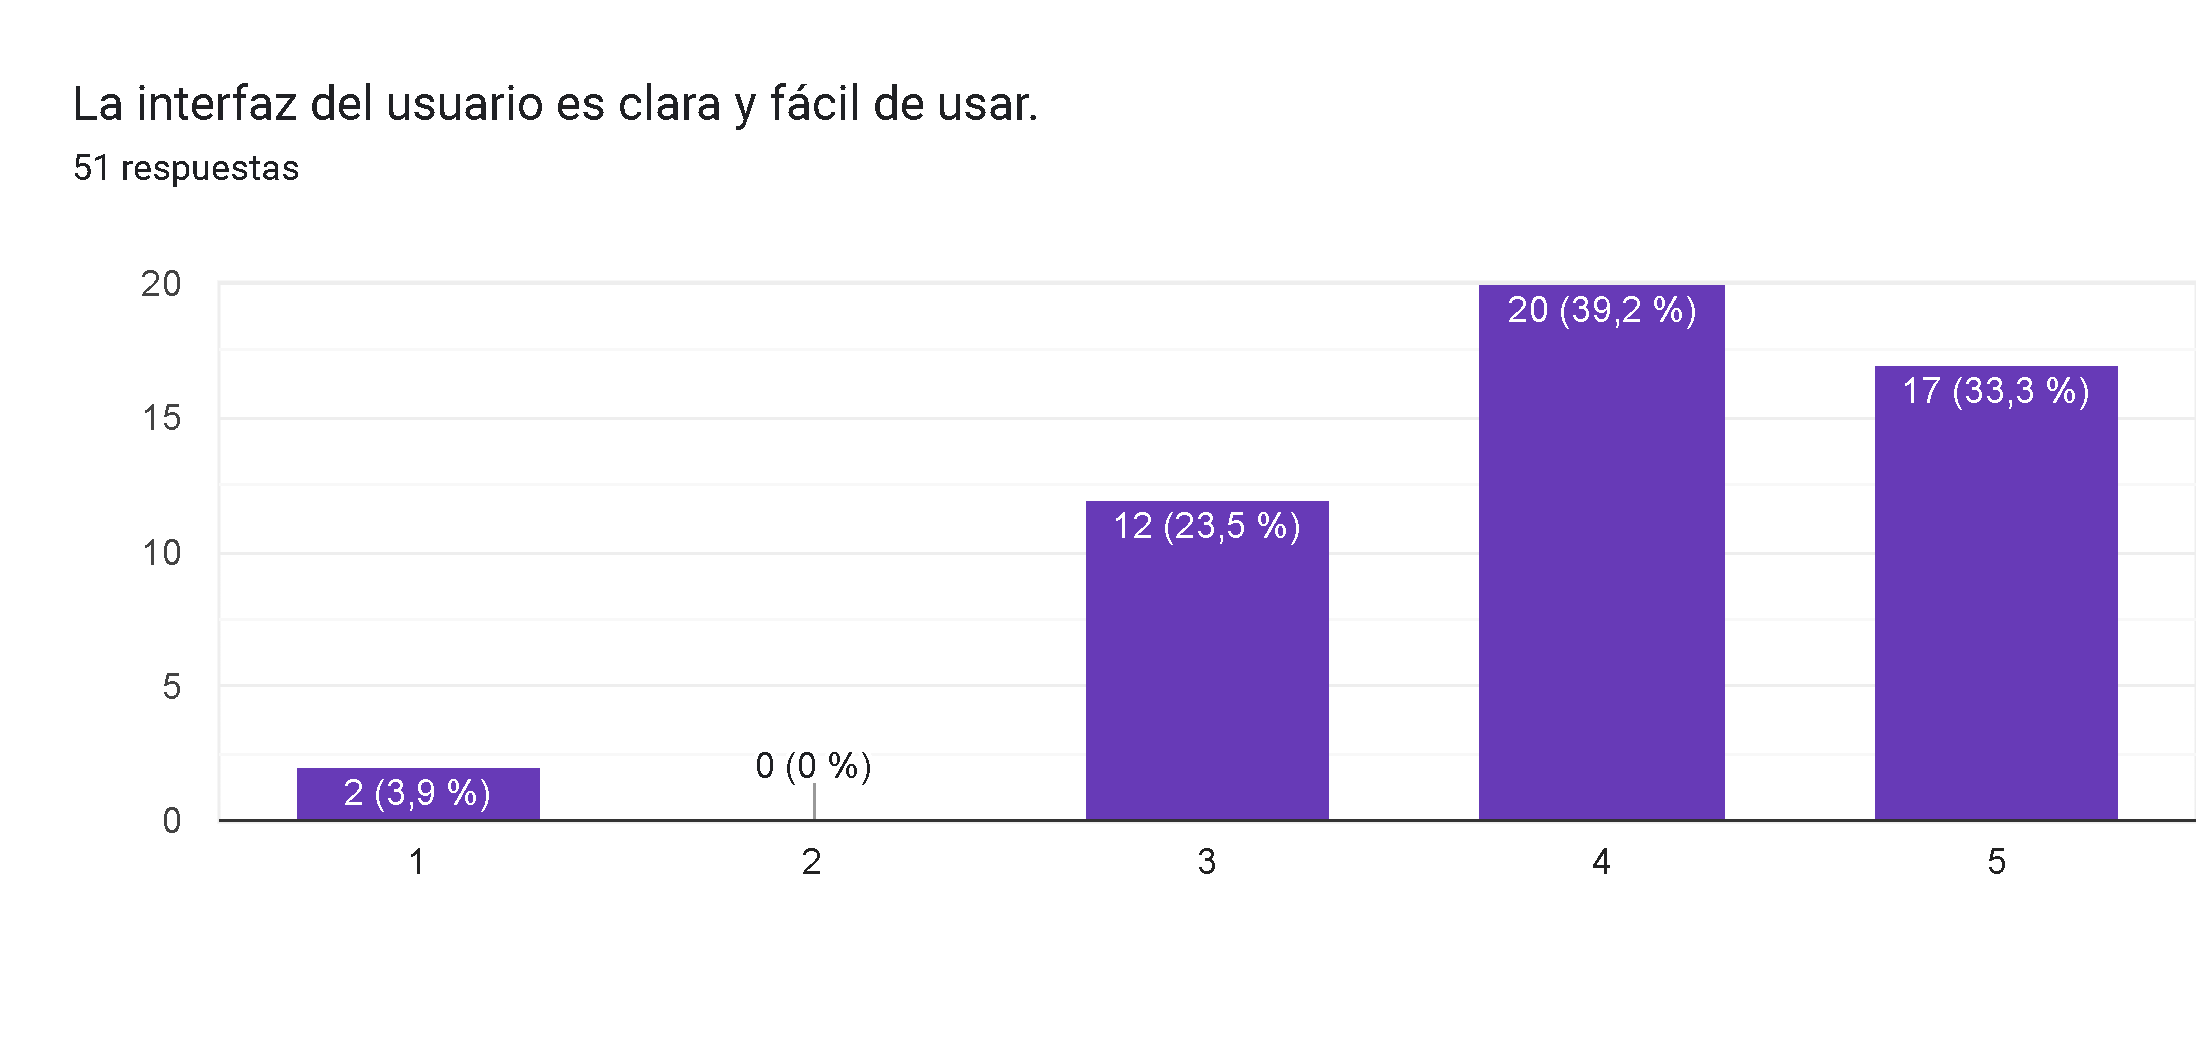
\includegraphics[width=0.7\linewidth]{Imagenes/fd6.png}
  \caption{Elaboración propia, Módulo fitness, Imagen de referencia sobre cuestionario de gamificación para el módulo fitness del juego sobre el movimiento de la espalda, ``La interfaz del usuario es clara y fácil de usar``}
  \label{fig:cuestionario17fitness}
\end{figure}

La pregunta ``La música del juego es adecuada y mejora la experiencia`` tuvo una buena recepción, con la mayoría de las respuestas mayores a 4. Esto indica que, aparentemente, la música fue del agrado de los jugadores y contribuyó positivamente a su experiencia.

\begin{figure}[H]
  \centering
  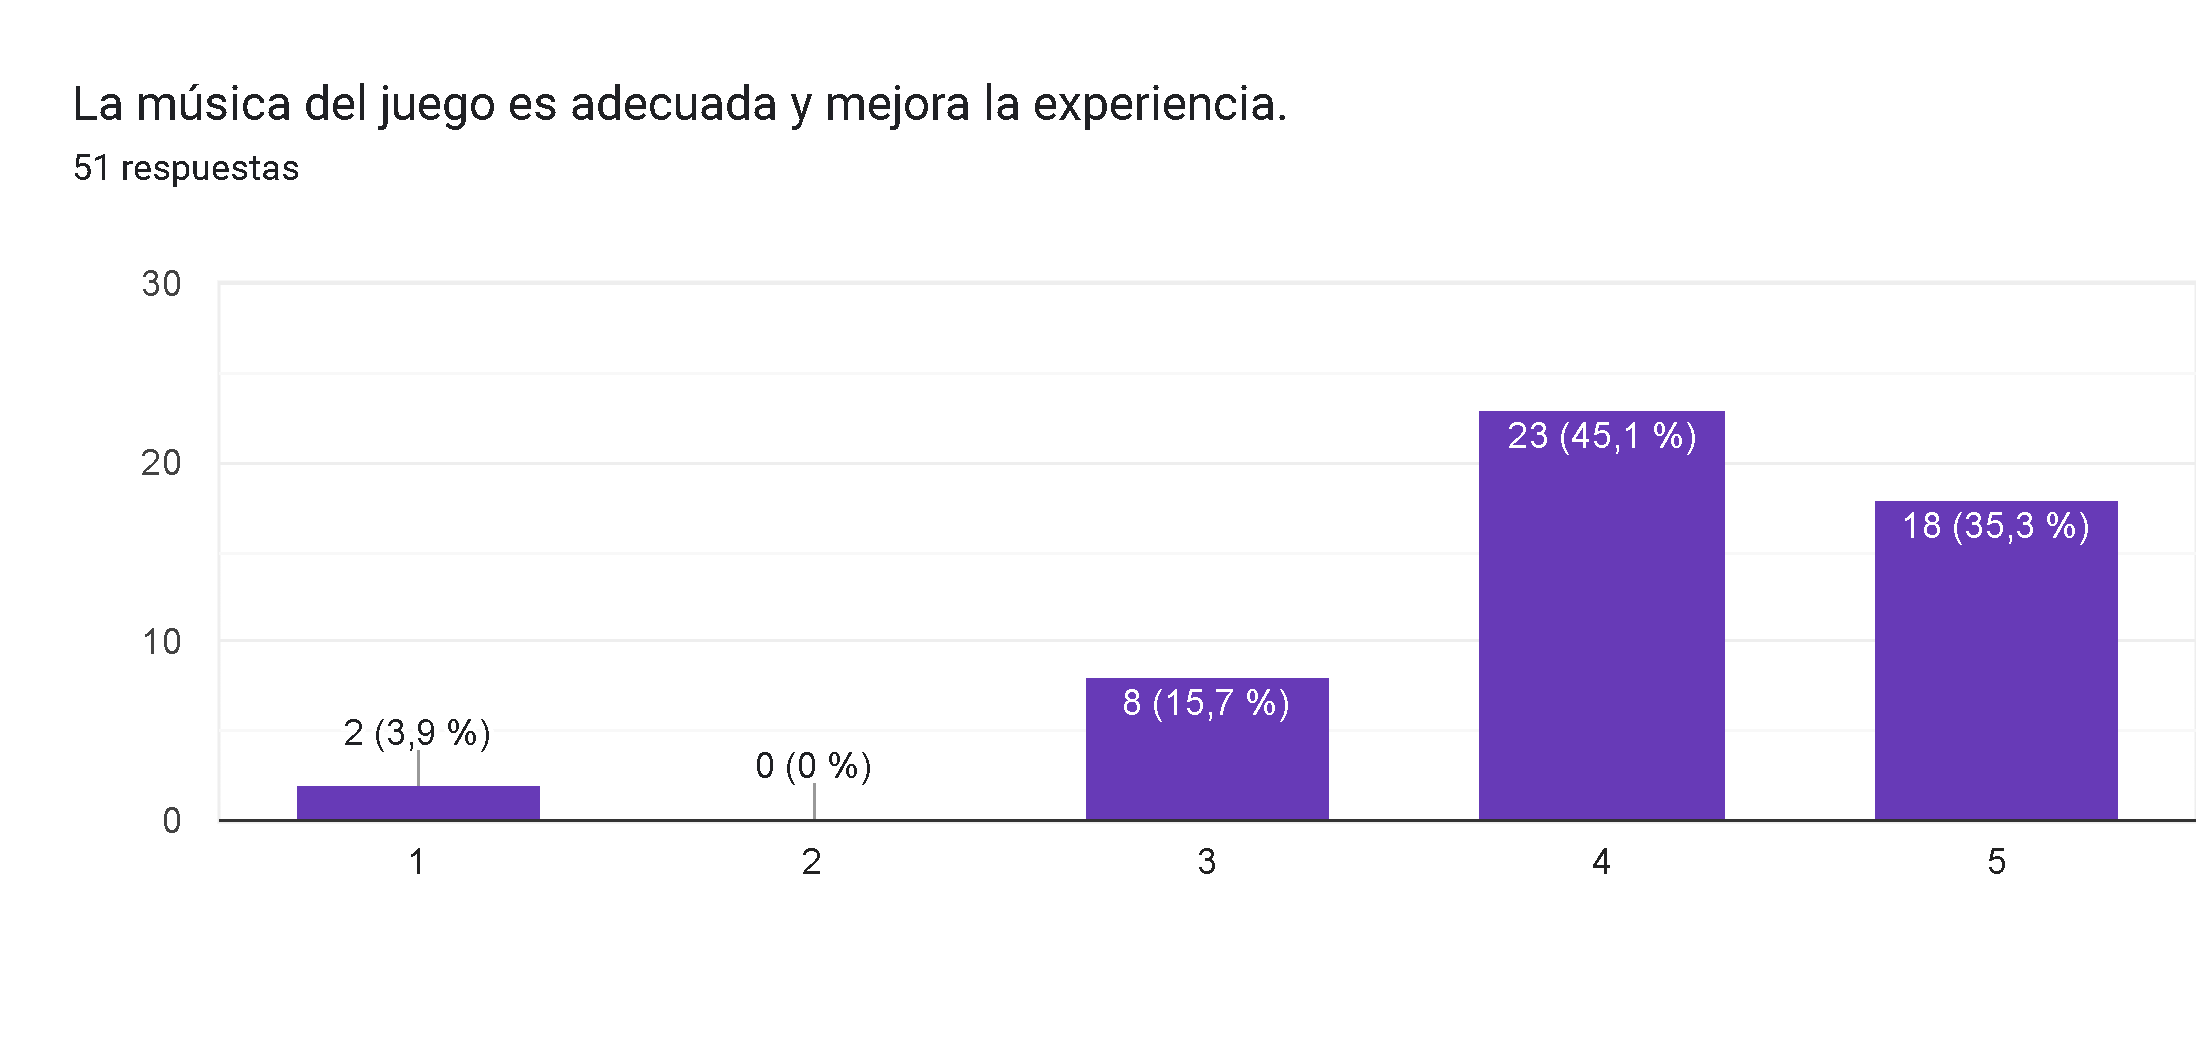
\includegraphics[width=0.7\linewidth]{Imagenes/fd7.png}
  \caption{Elaboración propia, Módulo fitness, Imagen de referencia sobre cuestionario de gamificación para el módulo fitness del juego sobre el movimiento de la espalda, ``La música del juego es adecuada y mejora la experiencia``}
  \label{fig:cuestionario18fitness}
\end{figure}


La pregunta ``El juego se ejecuta sin problemas de rendimiento (lag, caídas de FPS, etc.)`` obtuvo la mayor cantidad de respuestas en la opción 4, con un 41,2 \%. También se observó un 25,5 \% en la opción 3, lo que sugiere que la mayoría de los usuarios experimenta un buen rendimiento, aunque un grupo considerable podría haber notado leves problemas en el rendimiento.

\begin{figure}[H]
  \centering
  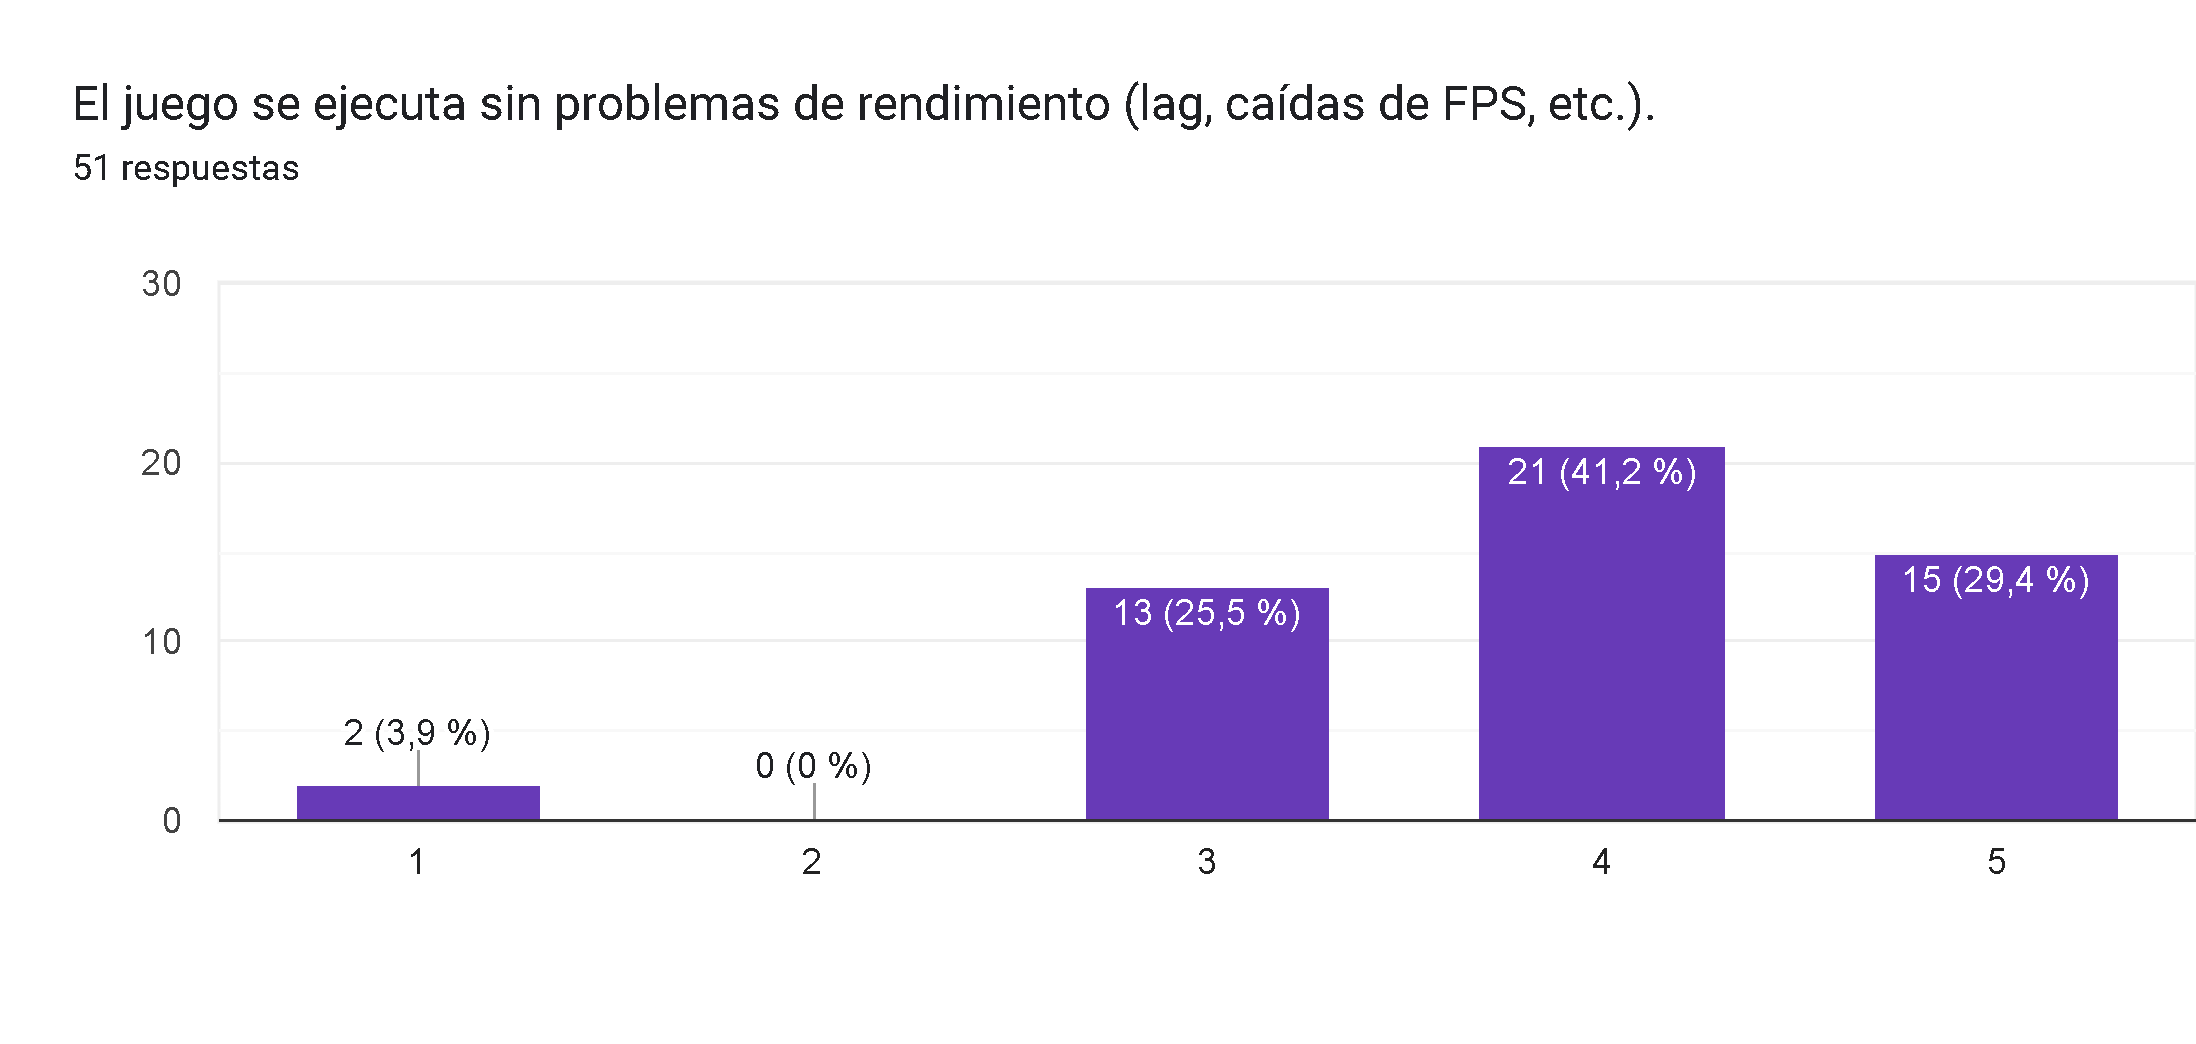
\includegraphics[width=0.7\linewidth]{Imagenes/fd8.png}
  \caption{Elaboración propia, Módulo fitness, Imagen de referencia sobre cuestionario de gamificación para el módulo fitness del juego sobre el movimiento de la espalda, ``El juego se ejecuta sin problemas de rendimiento (lag, caídas de FPS, etc.)``}
  \label{fig:cuestionario19fitness}
\end{figure}

La pregunta ``No he experimentado fallos técnicos o bugs importantes`` obtuvo la mayor cantidad de respuestas en la opción 4, con un 43,1 \%. Además, un 19,6 \% eligió la opción 3, lo que sugiere que la mayoría de los usuarios no han experimentado fallos importantes, aunque un porcentaje significativo aún podría haber encontrado errores menores o bugs en el juego.

\begin{figure}[H]
  \centering
  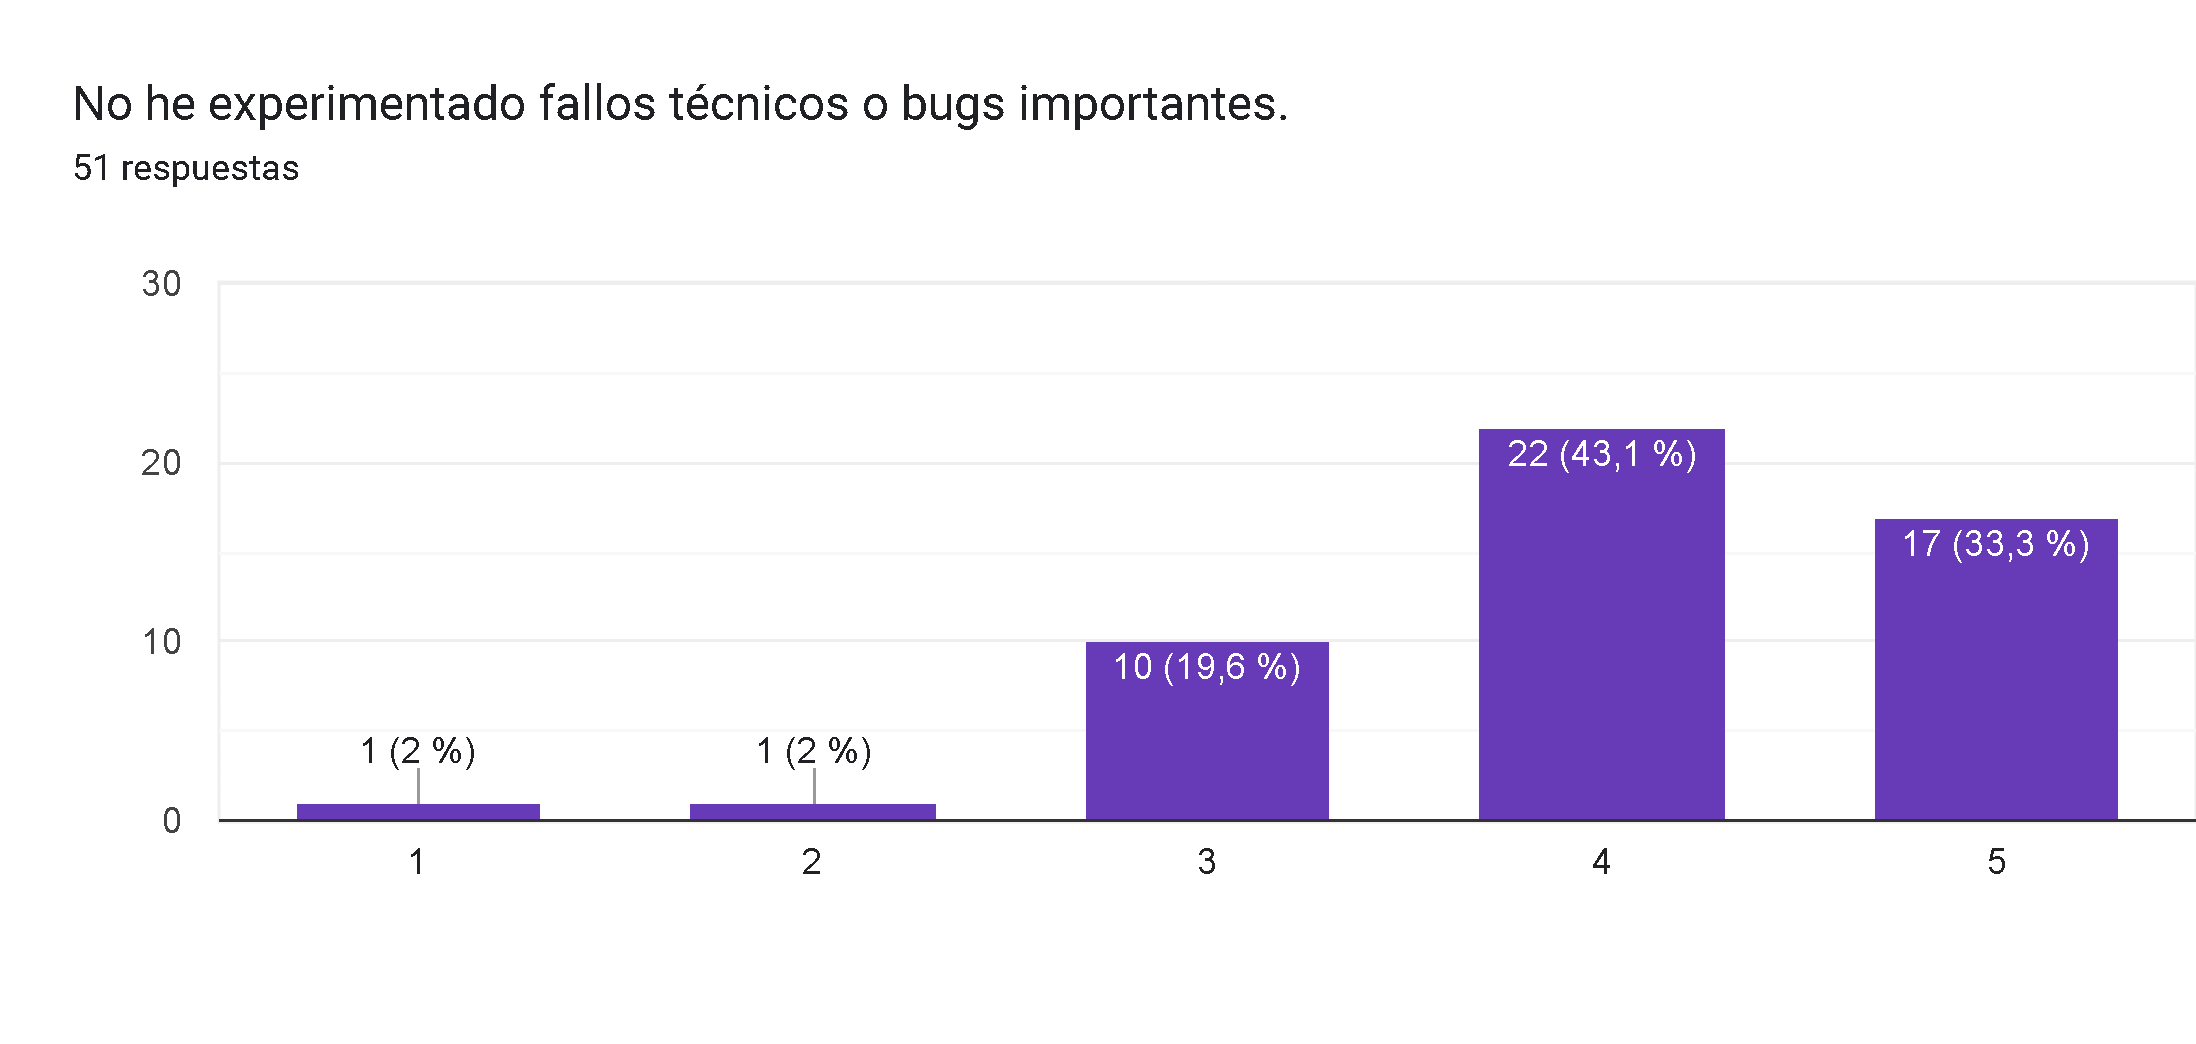
\includegraphics[width=0.7\linewidth]{Imagenes/fd9.png}
  \caption{Elaboración propia, Módulo fitness, Imagen de referencia sobre cuestionario de gamificación para el módulo fitness del juego sobre el movimiento de la espalda, ``No he experimentado fallos técnicos o bugs importantes``}
  \label{fig:cuestionario20fitness}
\end{figure}


La pregunta ``El juego me ha mantenido motivado para seguir jugando`` obtuvo la mayor cantidad de respuestas en la opción 4, con un 41,7 \%. Además, un 31,3 \% de los usuarios eligieron la opción 3, lo que indica que la mayoría se siente motivada para continuar jugando, aunque algunos aún podrían necesitar más incentivos.

\begin{figure}[H]
  \centering
  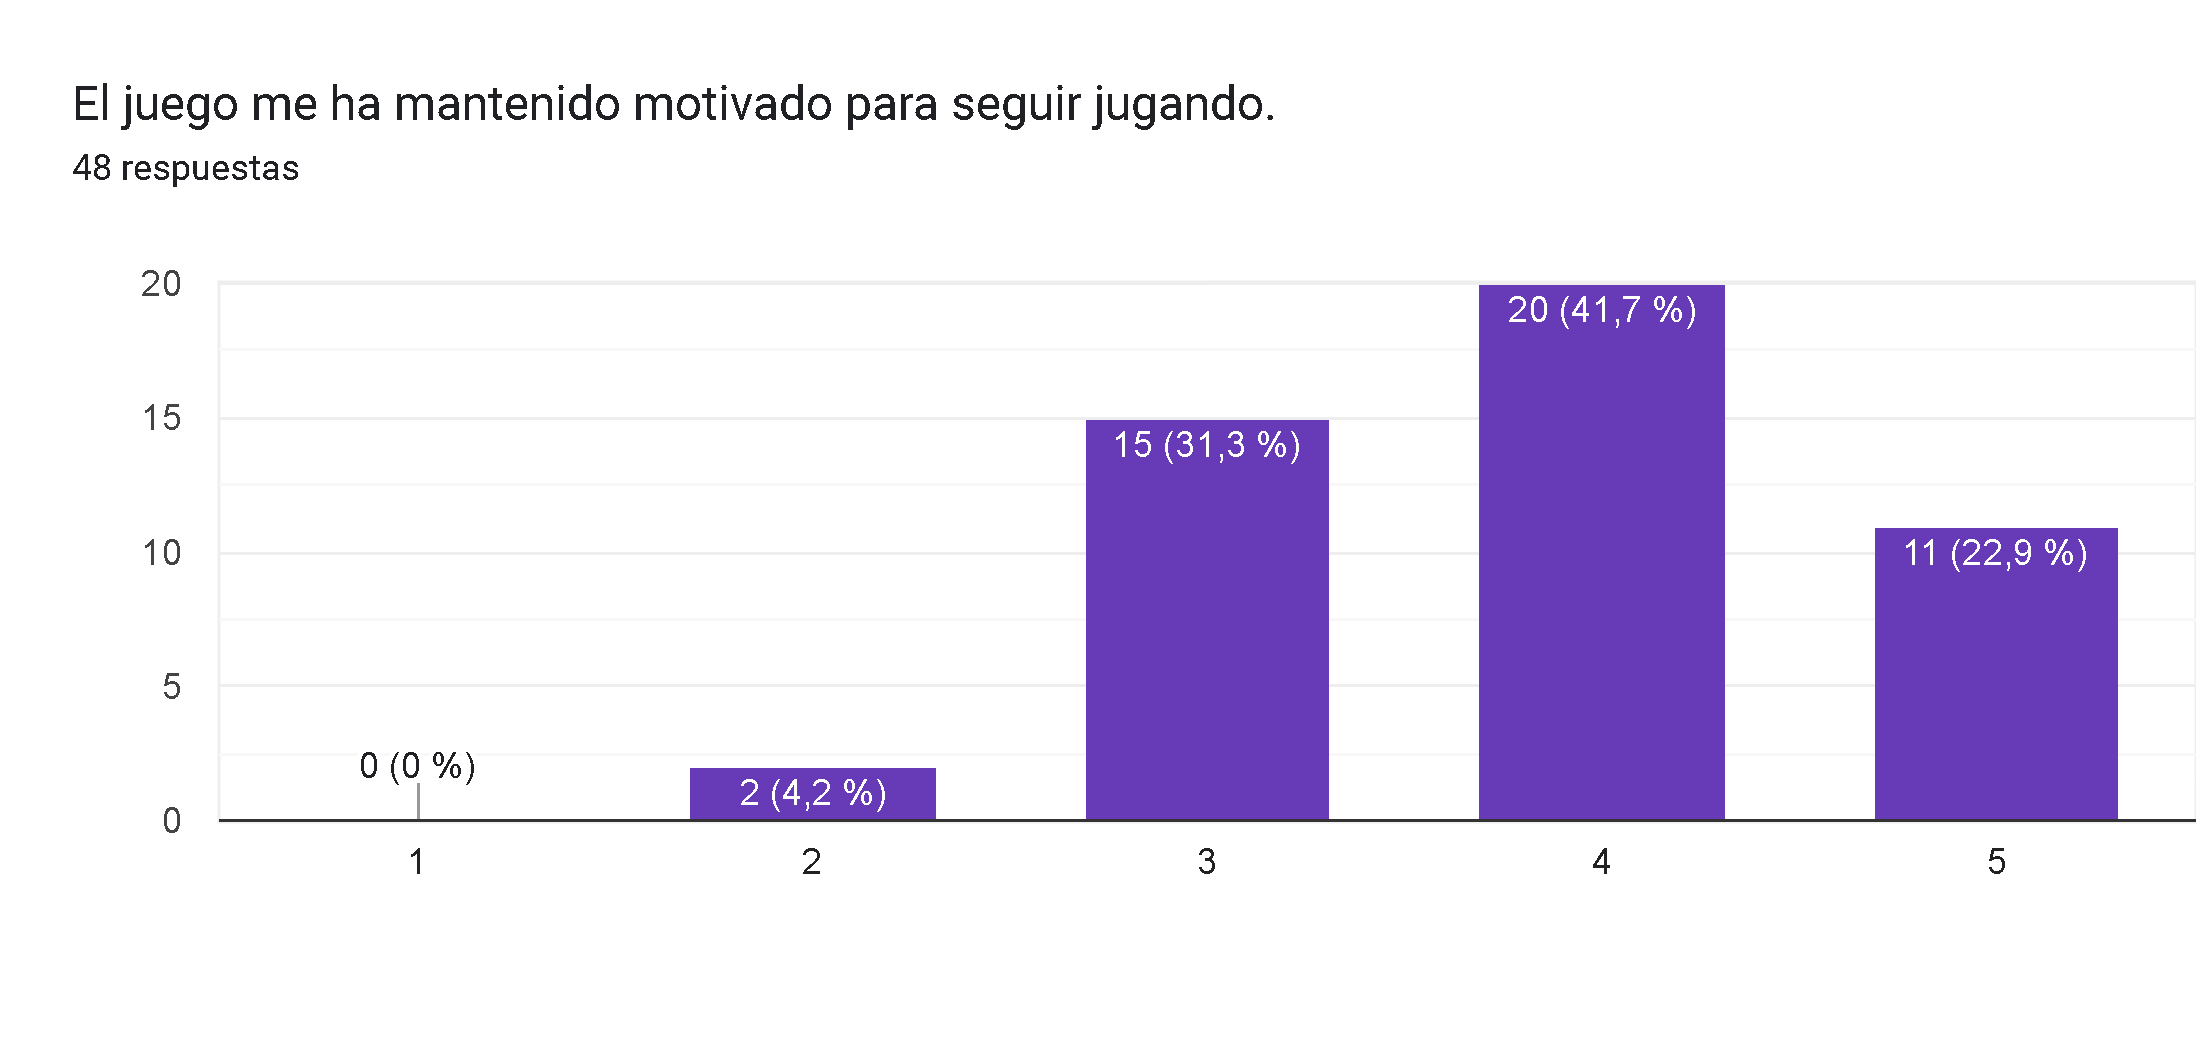
\includegraphics[width=0.7\linewidth]{Imagenes/fd10.png}
  \caption{Elaboración propia, Módulo fitness, Imagen de referencia sobre cuestionario de gamificación para el módulo fitness del juego sobre el movimiento de la espalda, ``El juego me ha mantenido motivado para seguir jugando``}
  \label{fig:cuestionario21fitness}
\end{figure}

La pregunta ``Consideras que el juego es útil para ayudar a la prevención de dolores articulares basados en la espalda`` obtuvo la mayor cantidad de respuestas en la opción 4, con un 47,1 \%, seguida de un 39,2 \% en la opción 5. Esto indica que una mayoría de los usuarios considera que el juego puede ser útil para la prevención de dolores articulares en la espalda, aunque un porcentaje significativo aún tiene dudas al respecto.

\begin{figure}[H]
  \centering
  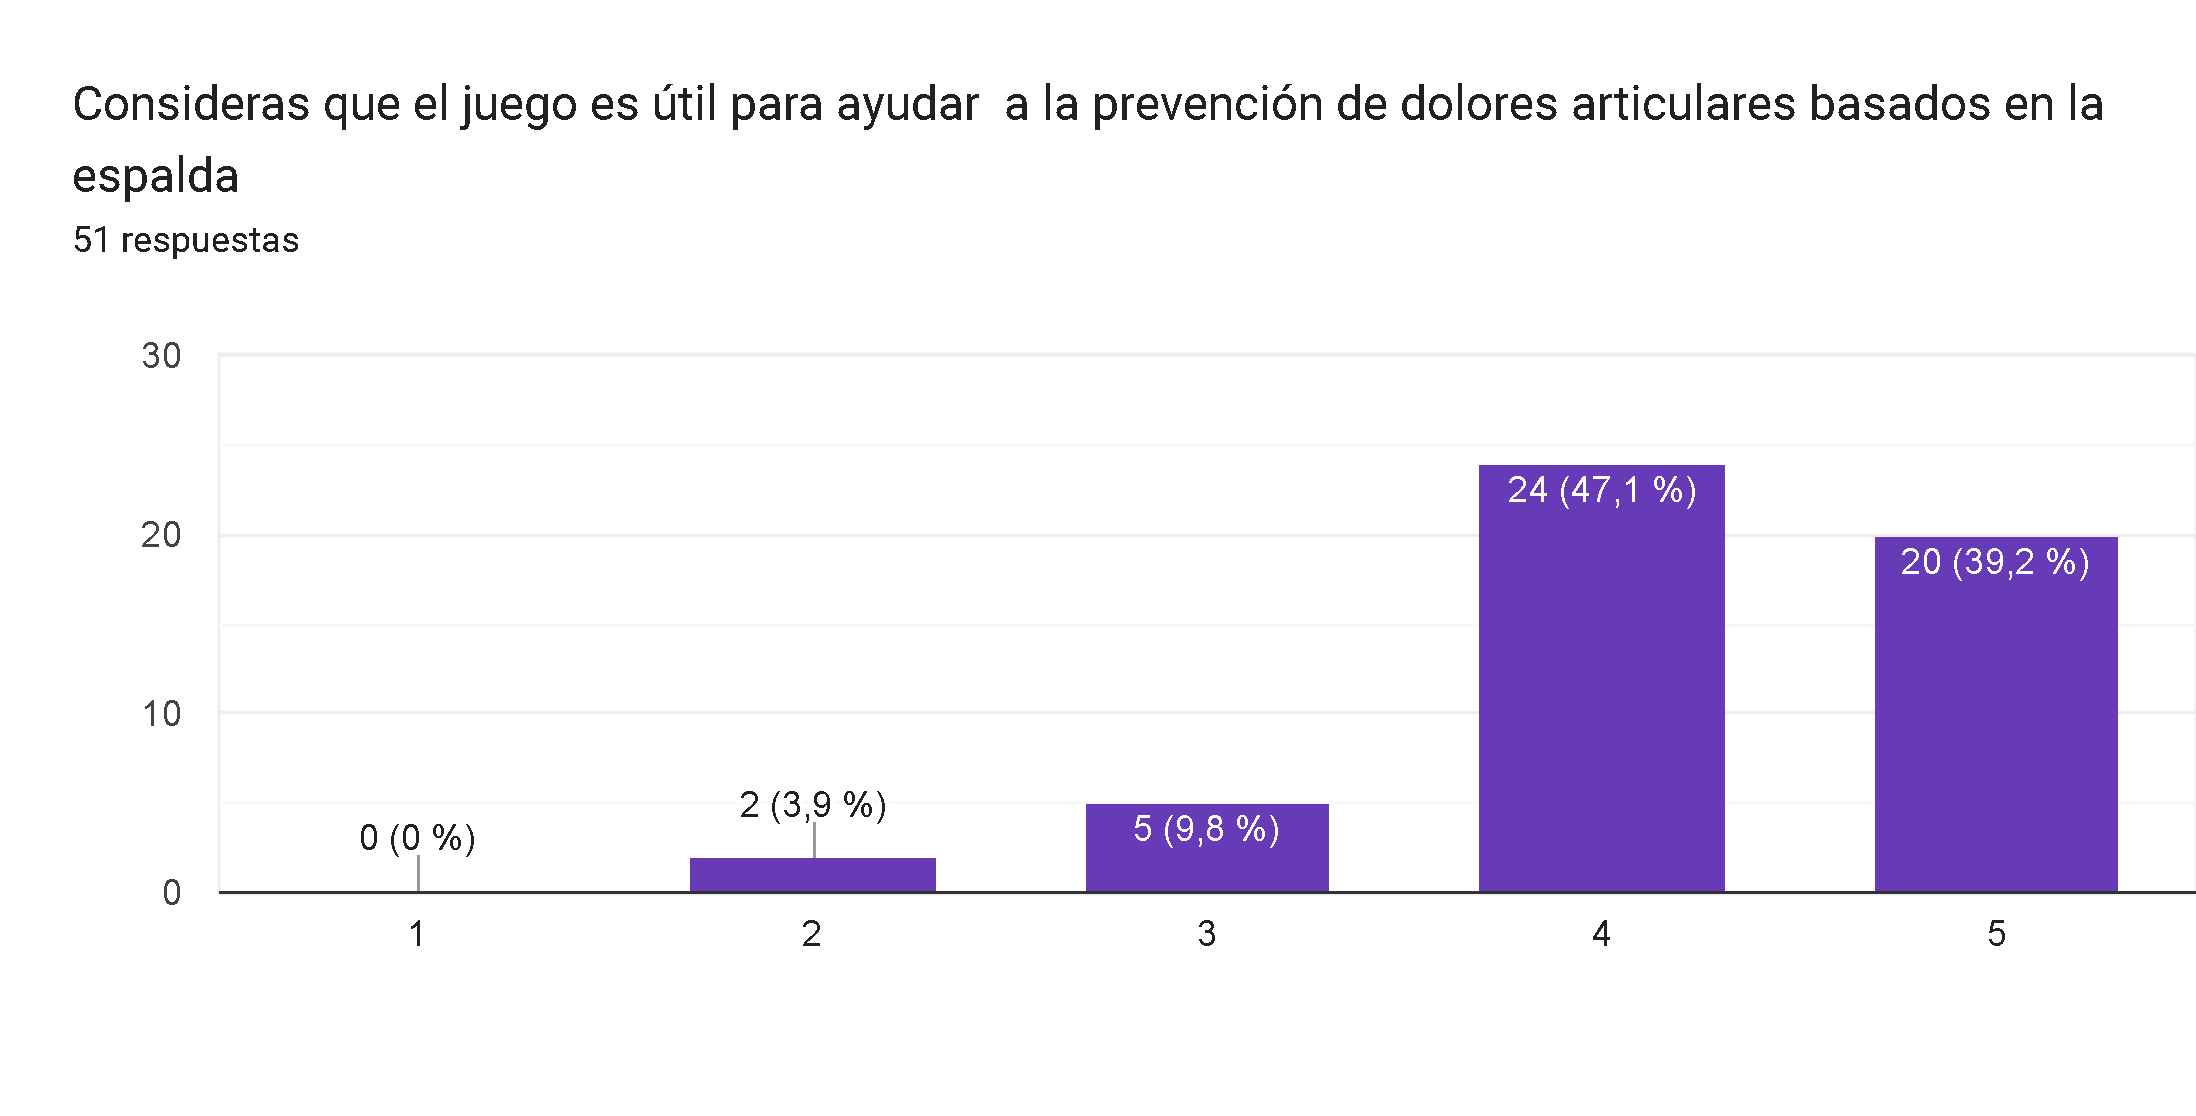
\includegraphics[width=0.7\linewidth]{Imagenes/fd11.png}
  \caption{Elaboración propia, Módulo fitness, Imagen de referencia sobre cuestionario de gamificación para el módulo fitness del juego sobre el movimiento de la espalda, ``Consideras que el juego es útil para ayudar a la prevención de dolores articulares basados en la espalda``}
  \label{fig:cuestionario22fitness}
\end{figure}


La pregunta ``Me siento satisfecho con la experiencia general del juego`` obtuvo la mayor cantidad de respuestas en la opción 4, con un 49 \%, seguida de un 25,5 \% en la opción 5, y de un 21,6 \% en la opción 3. Esto sugiere que la mayoría de los usuarios están satisfechos con la experiencia general del juego, aunque un porcentaje considerable podría tener áreas de mejora o expectativas aún no completamente satisfechas.

\begin{figure}[H]
  \centering
  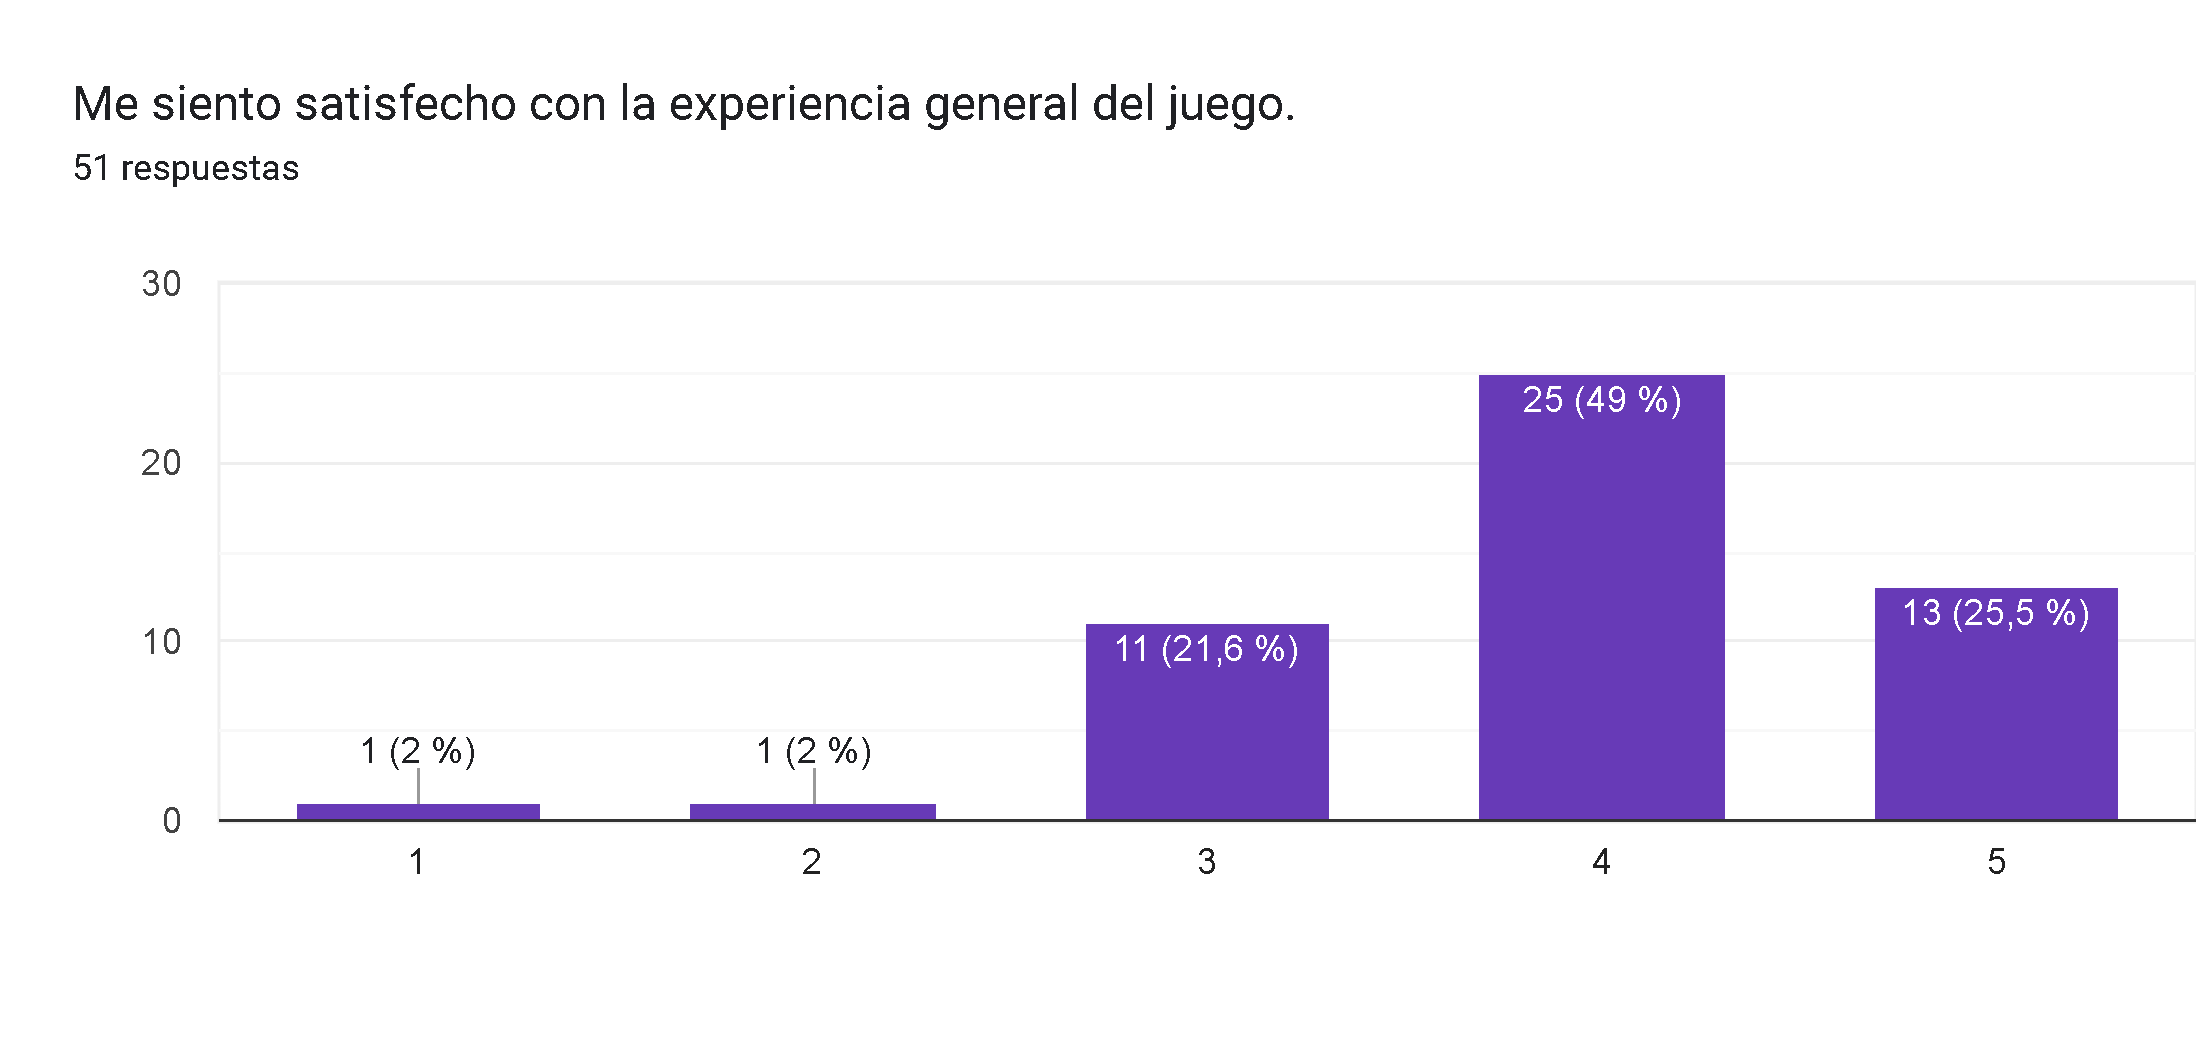
\includegraphics[width=0.7\linewidth]{Imagenes/fd12.png}
  \caption{Elaboración propia, Módulo fitness, Imagen de referencia sobre cuestionario de gamificación para el módulo fitness del juego sobre el movimiento de la espalda, ``Me siento satisfecho con la experiencia general del juego``}
  \label{fig:cuestionario23fitness}
\end{figure}




\subsection{Mindset: Juego sobre puzzles}

La pregunta ``El juego es fácil de entender y aprender`` obtuvo la mayor cantidad de respuestas en la opción 5, con un 41,2 \%. Esto indica que la mayoría de los usuarios consideran que el juego es comprensible y fácil de aprender, aunque una parte también encuentra áreas que podrían mejorarse para facilitar aún más su comprensión.

\begin{figure}[H]
  \centering
  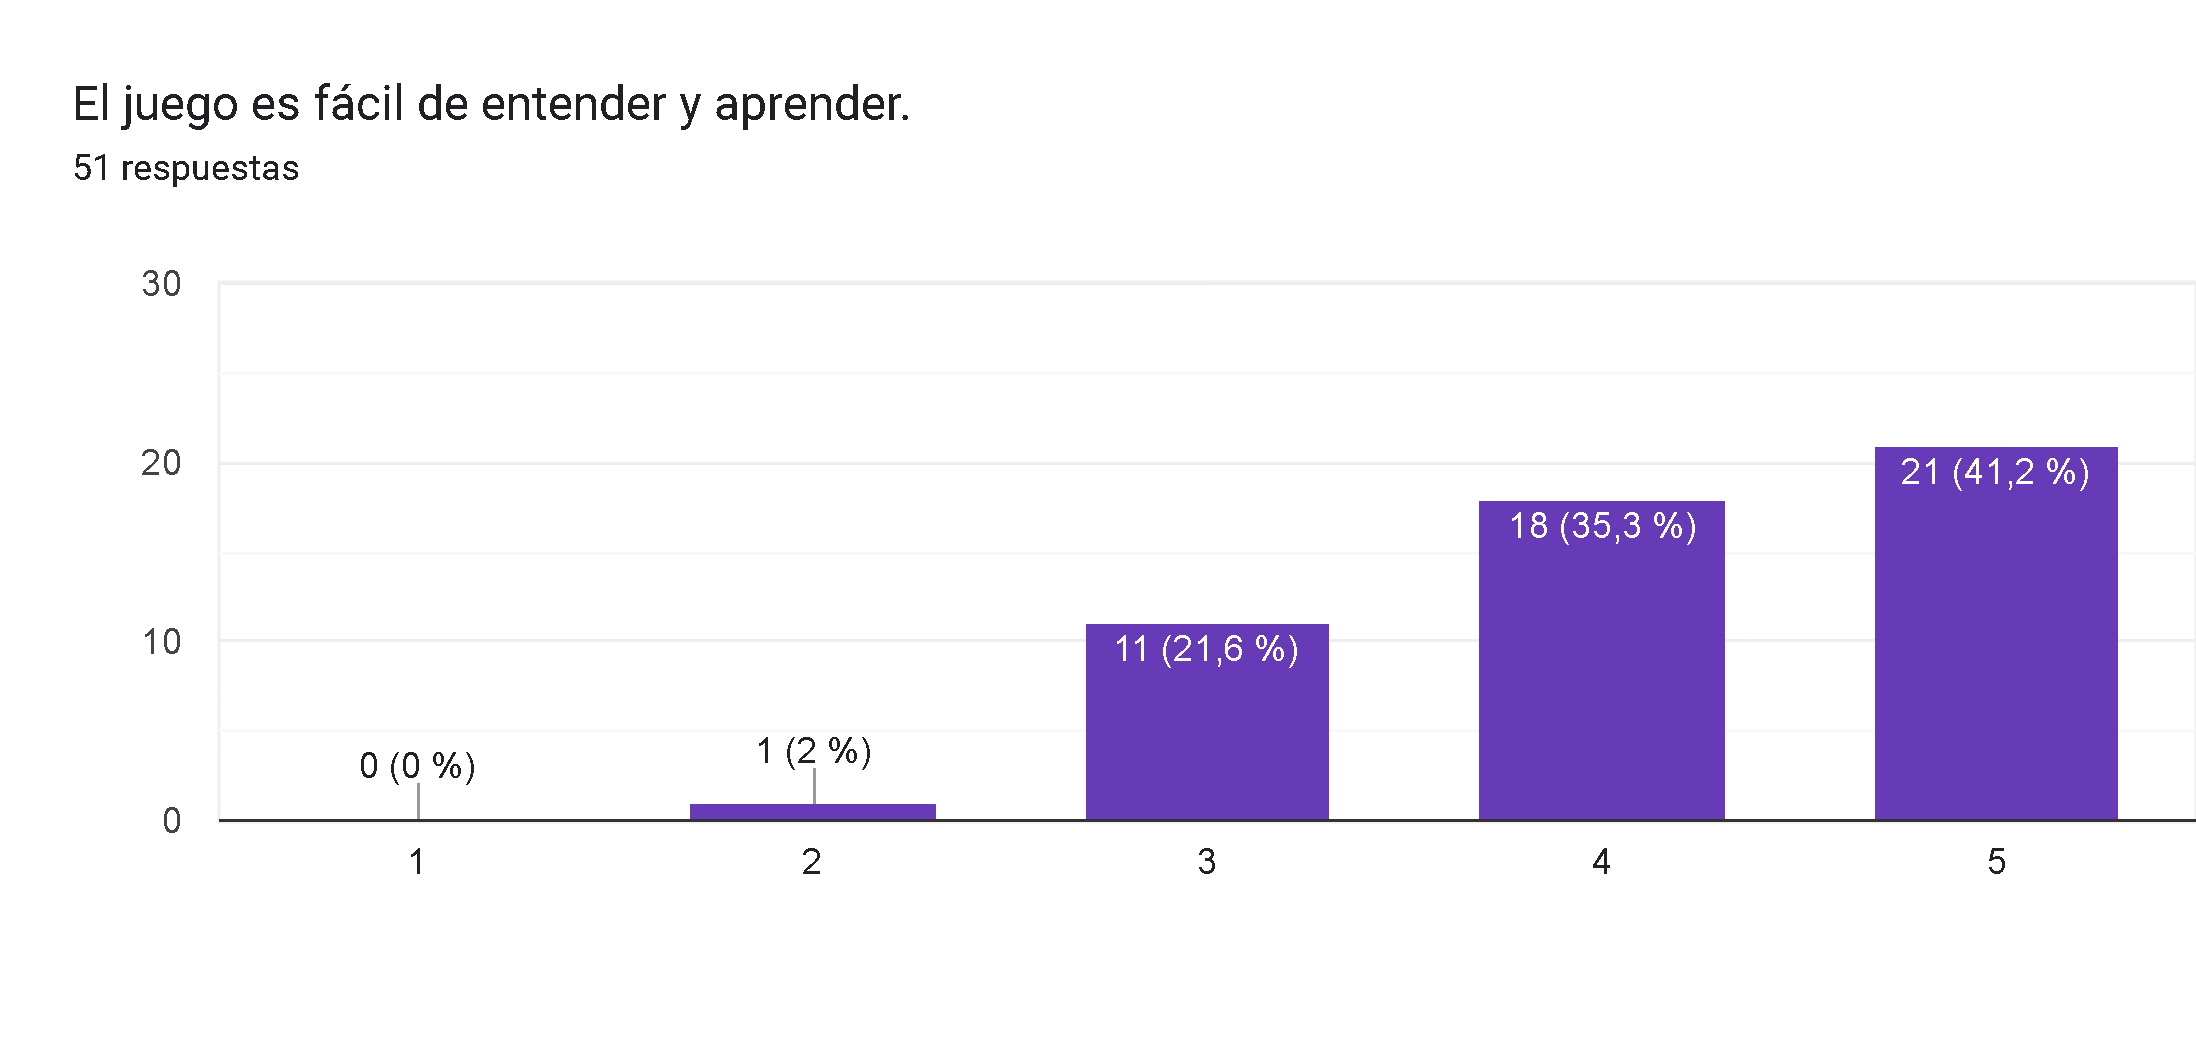
\includegraphics[width=0.7\linewidth]{Imagenes/mc1.png}
  \caption{Elaboración propia, Módulo mindset, Imagen de referencia sobre cuestionario de gamificación para el módulo mindset del juego sobre puzzles, ``El juego es fácil de entender y aprender``}
  \label{fig:cuestionario1mindset}
\end{figure}



La pregunta ``Los controles son intuitivos y responden bien`` obtuvo la mayor cantidad de respuestas en la opción 5, con un 39,2 \%. Esto sugiere que la mayoría de los usuarios consideran que los controles responden de manera adecuada y son fáciles de entender, mientras que un porcentaje considerable también seleccionó la opción 4, con un 37,3 \%, indicando una evaluación positiva pero con espacio para mejoras.

\begin{figure}[H]
  \centering
  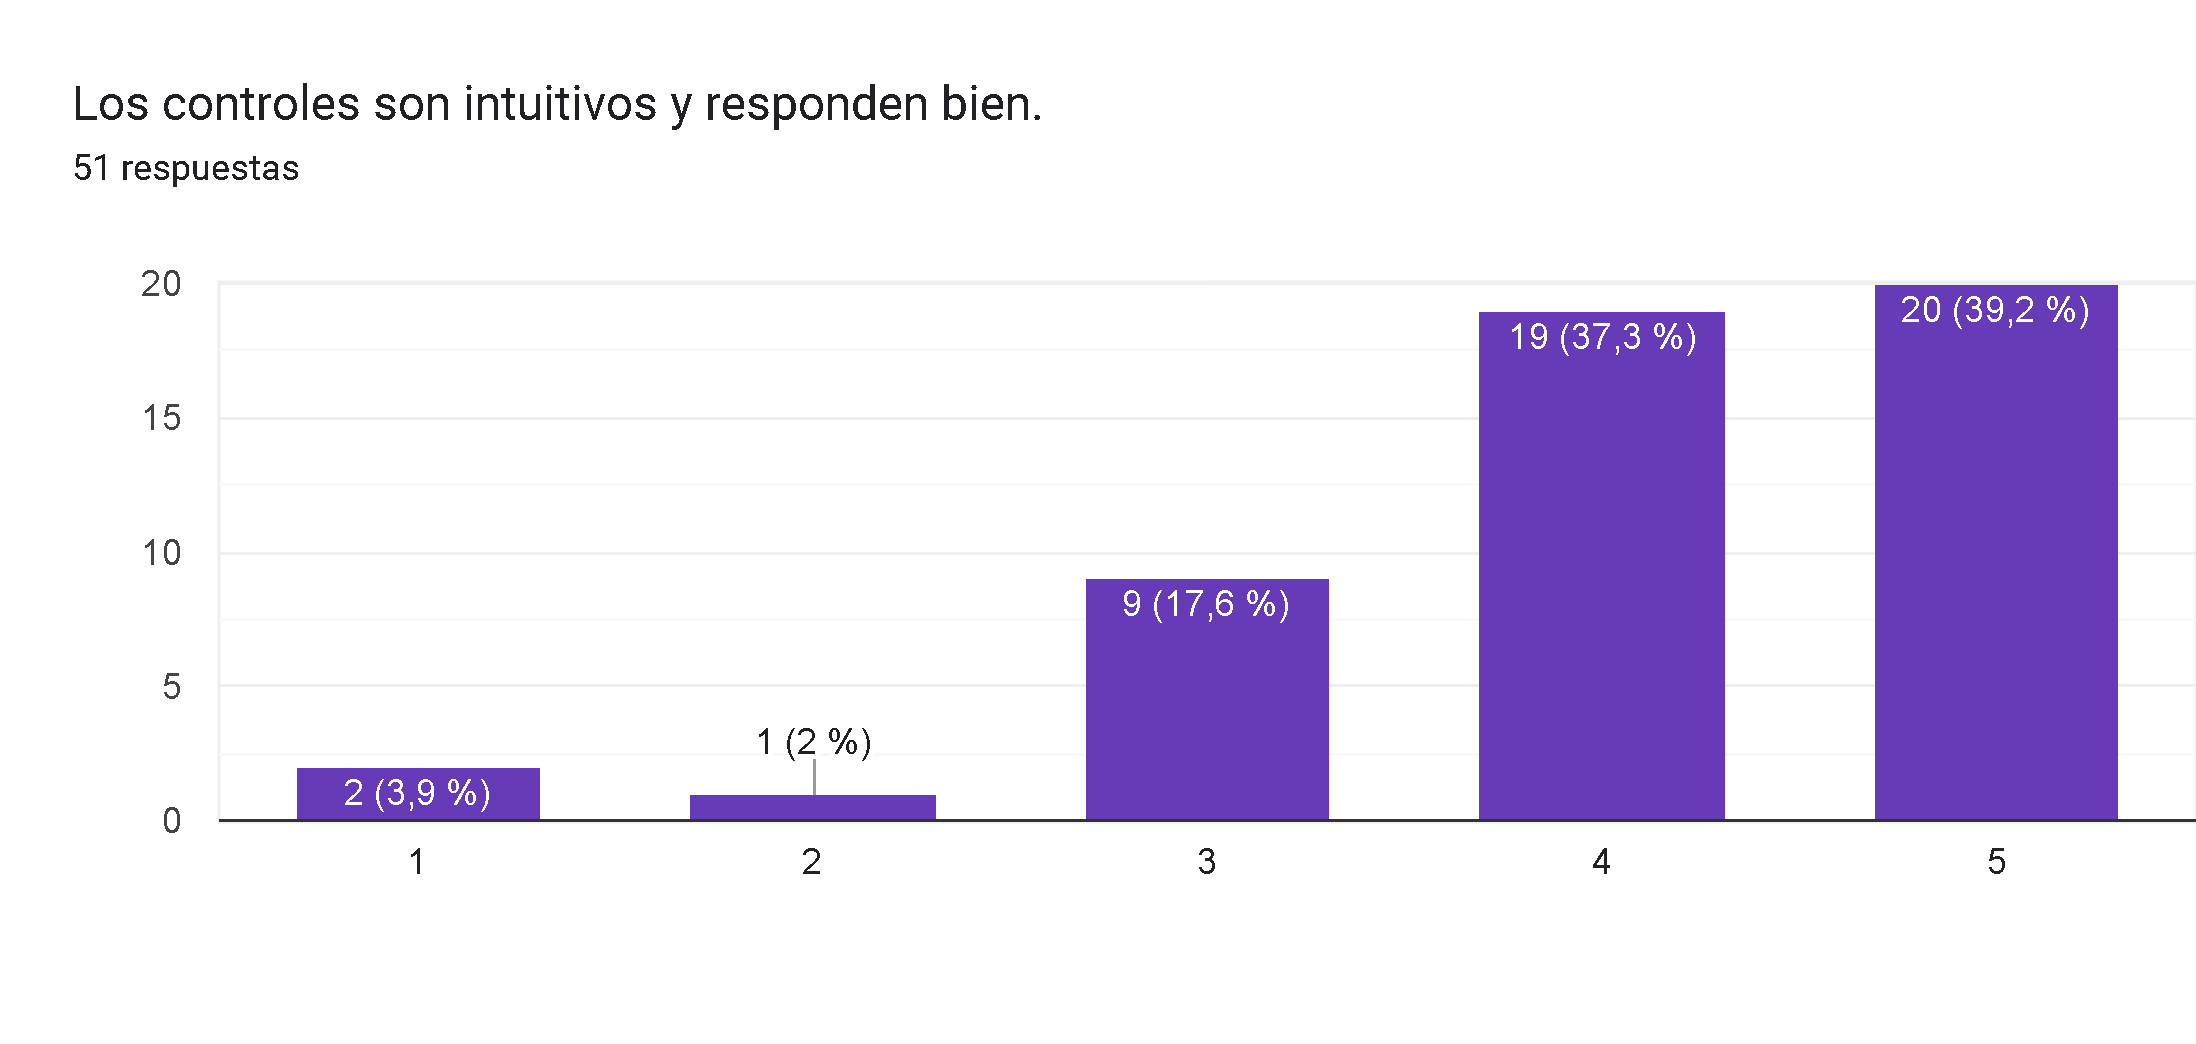
\includegraphics[width=0.7\linewidth]{Imagenes/mc2.png}
  \caption{Elaboración propia, Módulo mindset, Imagen de referencia sobre cuestionario de gamificación para el módulo mindset del juego sobre puzzles, ``Los controles son intuitivos y responden bien``}
  \label{fig:cuestionario2mindset}
\end{figure}

La pregunta ``El nivel de dificultad es adecuado`` obtuvo la mayor cantidad de respuestas en la opción 4, con un 47,1 \%. Esto sugiere que la mayoría de los usuarios consideran que el nivel de dificultad está bien equilibrado, proporcionando una experiencia desafiante pero no excesivamente difícil para la mayoría de los jugadores.

\begin{figure}[H]
  \centering
  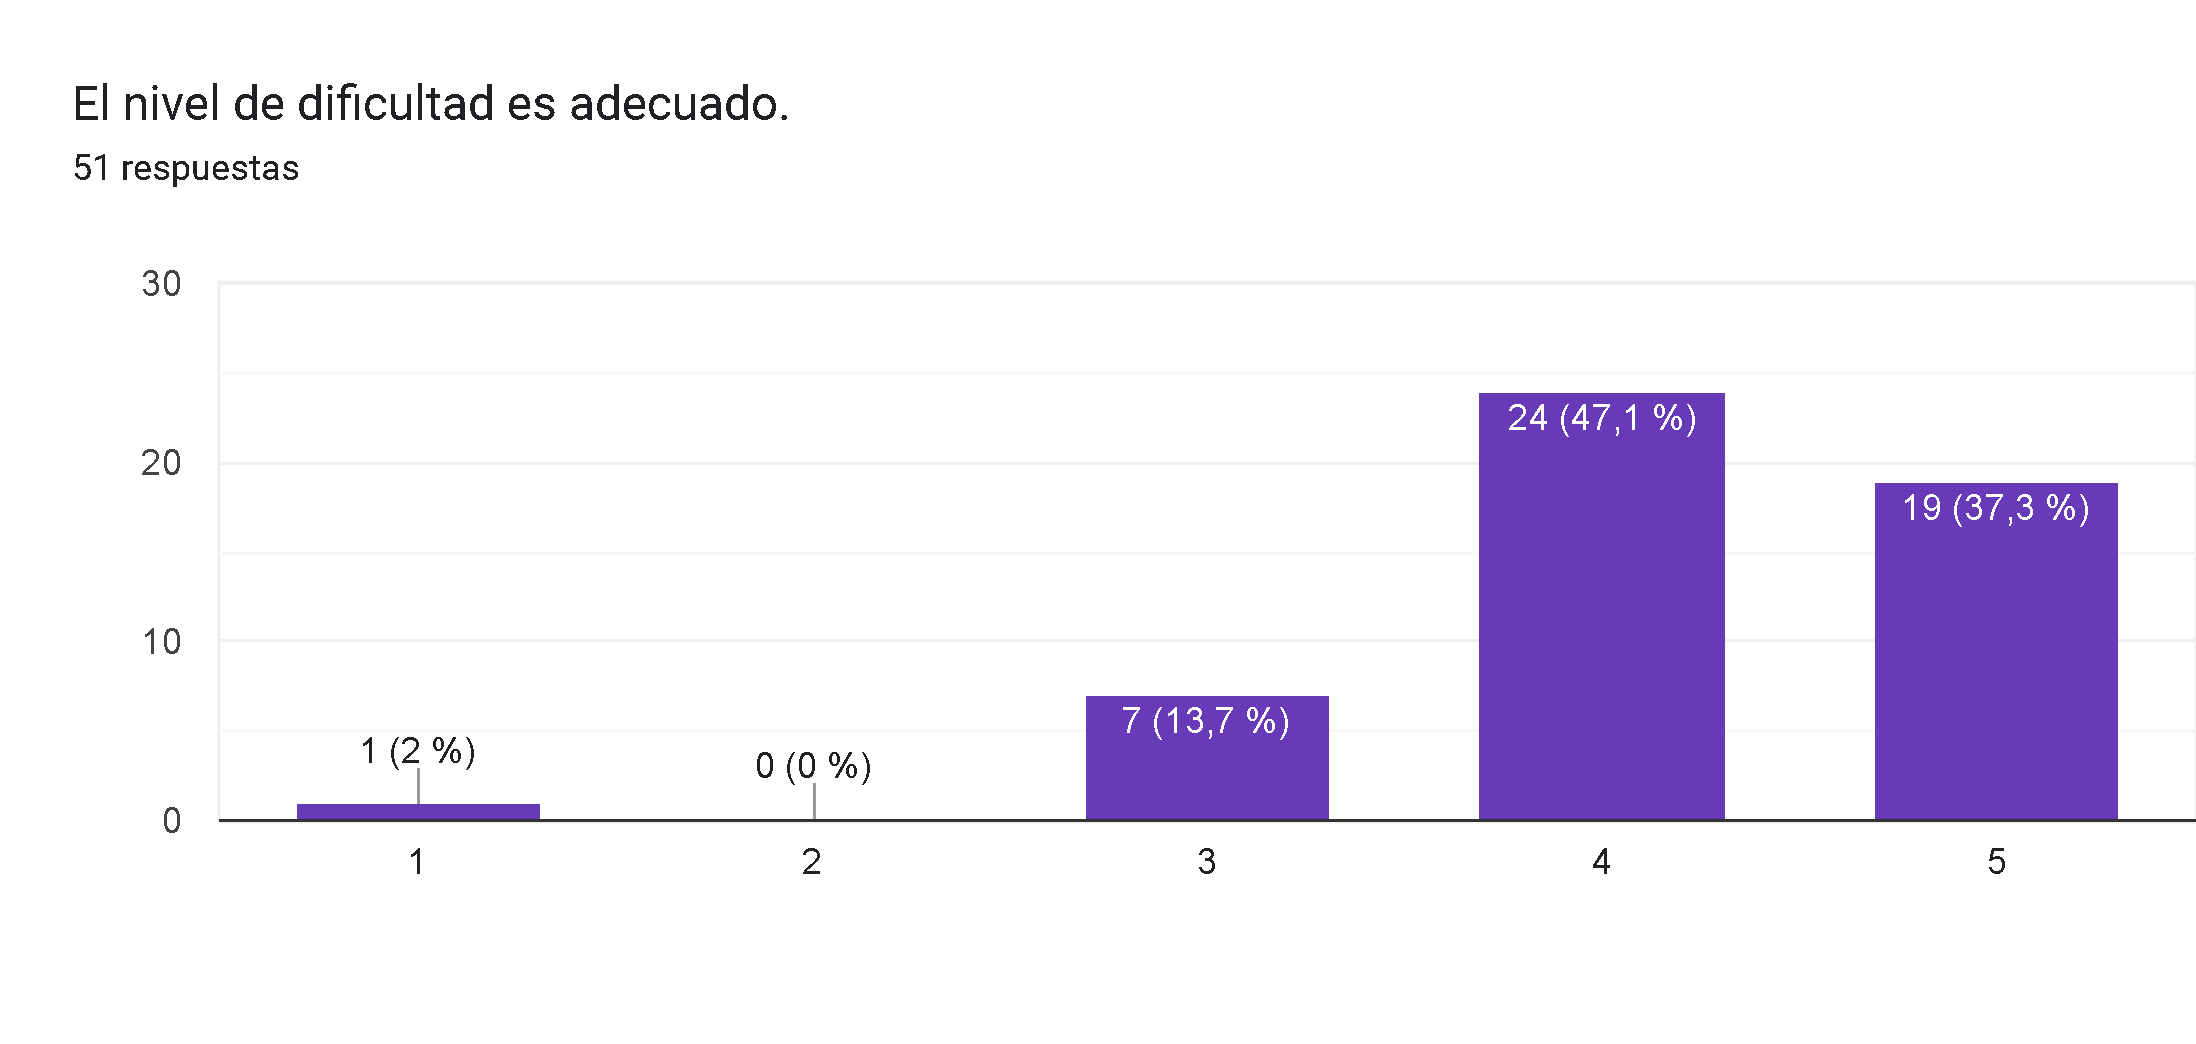
\includegraphics[width=0.7\linewidth]{Imagenes/mc3.png}
  \caption{Elaboración propia, Módulo mindset, Imagen de referencia sobre cuestionario de gamificación para el módulo mindset del juego sobre puzzles, ``El nivel de dificultad es adecuado``}
  \label{fig:cuestionario3mindset}
\end{figure}



La pregunta ``La interfaz del usuario es clara y fácil de usar`` obtuvo la mayor cantidad de respuestas en la opción 4, seguida de la opción 5. Esto indica que la mayoría de los usuarios encuentran la interfaz clara y fácil de usar, aunque un porcentaje también considera que podría haber áreas de mejora en su accesibilidad o claridad.

\begin{figure}[H]
  \centering
  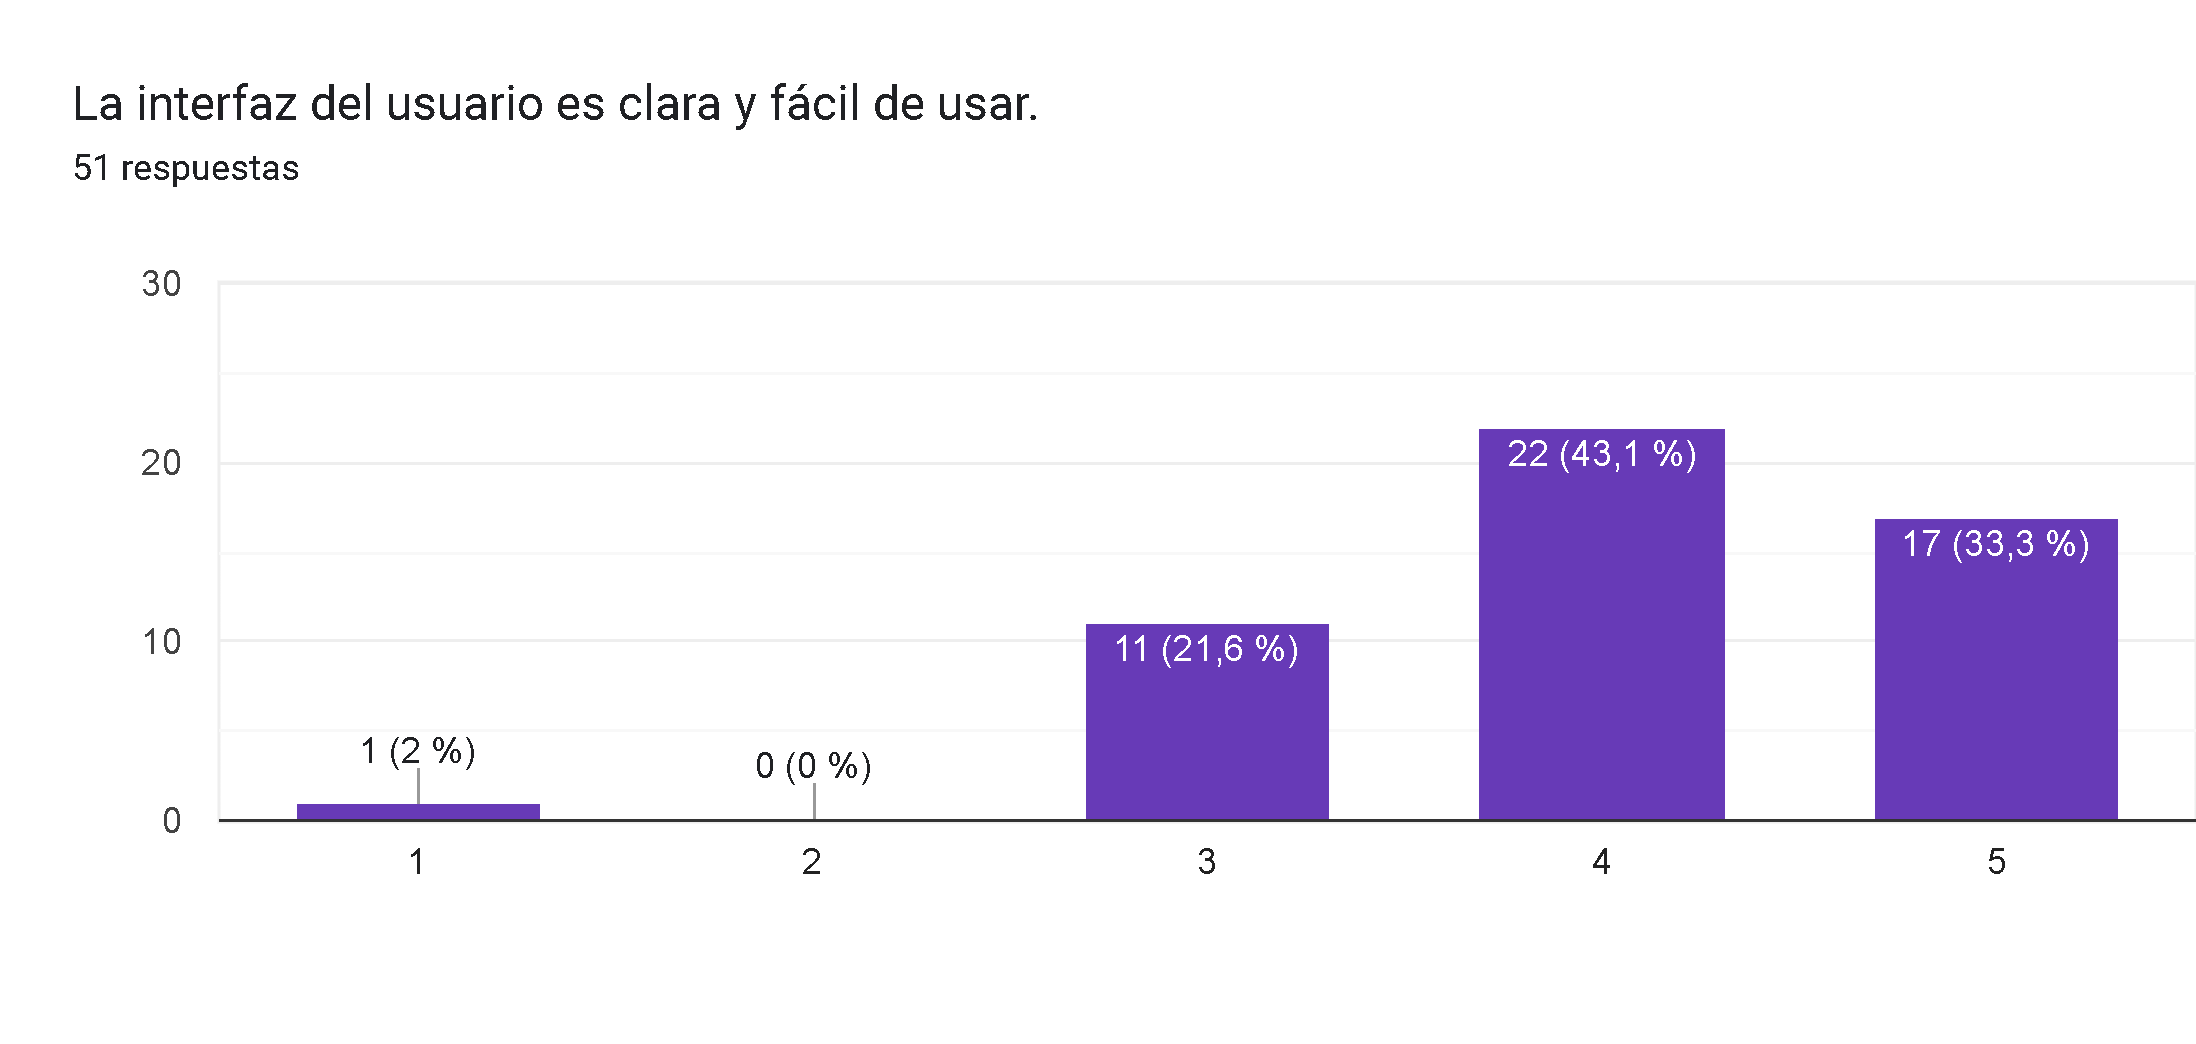
\includegraphics[width=0.7\linewidth]{Imagenes/mc4.png}
  \caption{Elaboración propia, Módulo mindset, Imagen de referencia sobre cuestionario de gamificación para el módulo mindset del juego sobre puzzles, ``La interfaz del usuario es clara y fácil de usar``}
  \label{fig:cuestionario4mindset}
\end{figure}

La pregunta ``La música del juego es adecuada y mejora la experiencia`` obtuvo la mayor cantidad de respuestas en la opción 4, con un 39,2 \%. La opción 3 recibió un 19,6 \%, mientras que un 35,3 \% optó por la opción 5. Esto sugiere que la mayoría de los usuarios considera que la música contribuye positivamente a la experiencia, aunque aún hay algunos que tienen dudas al respecto o consideran que puede mejorarse.

\begin{figure}[H]
  \centering
  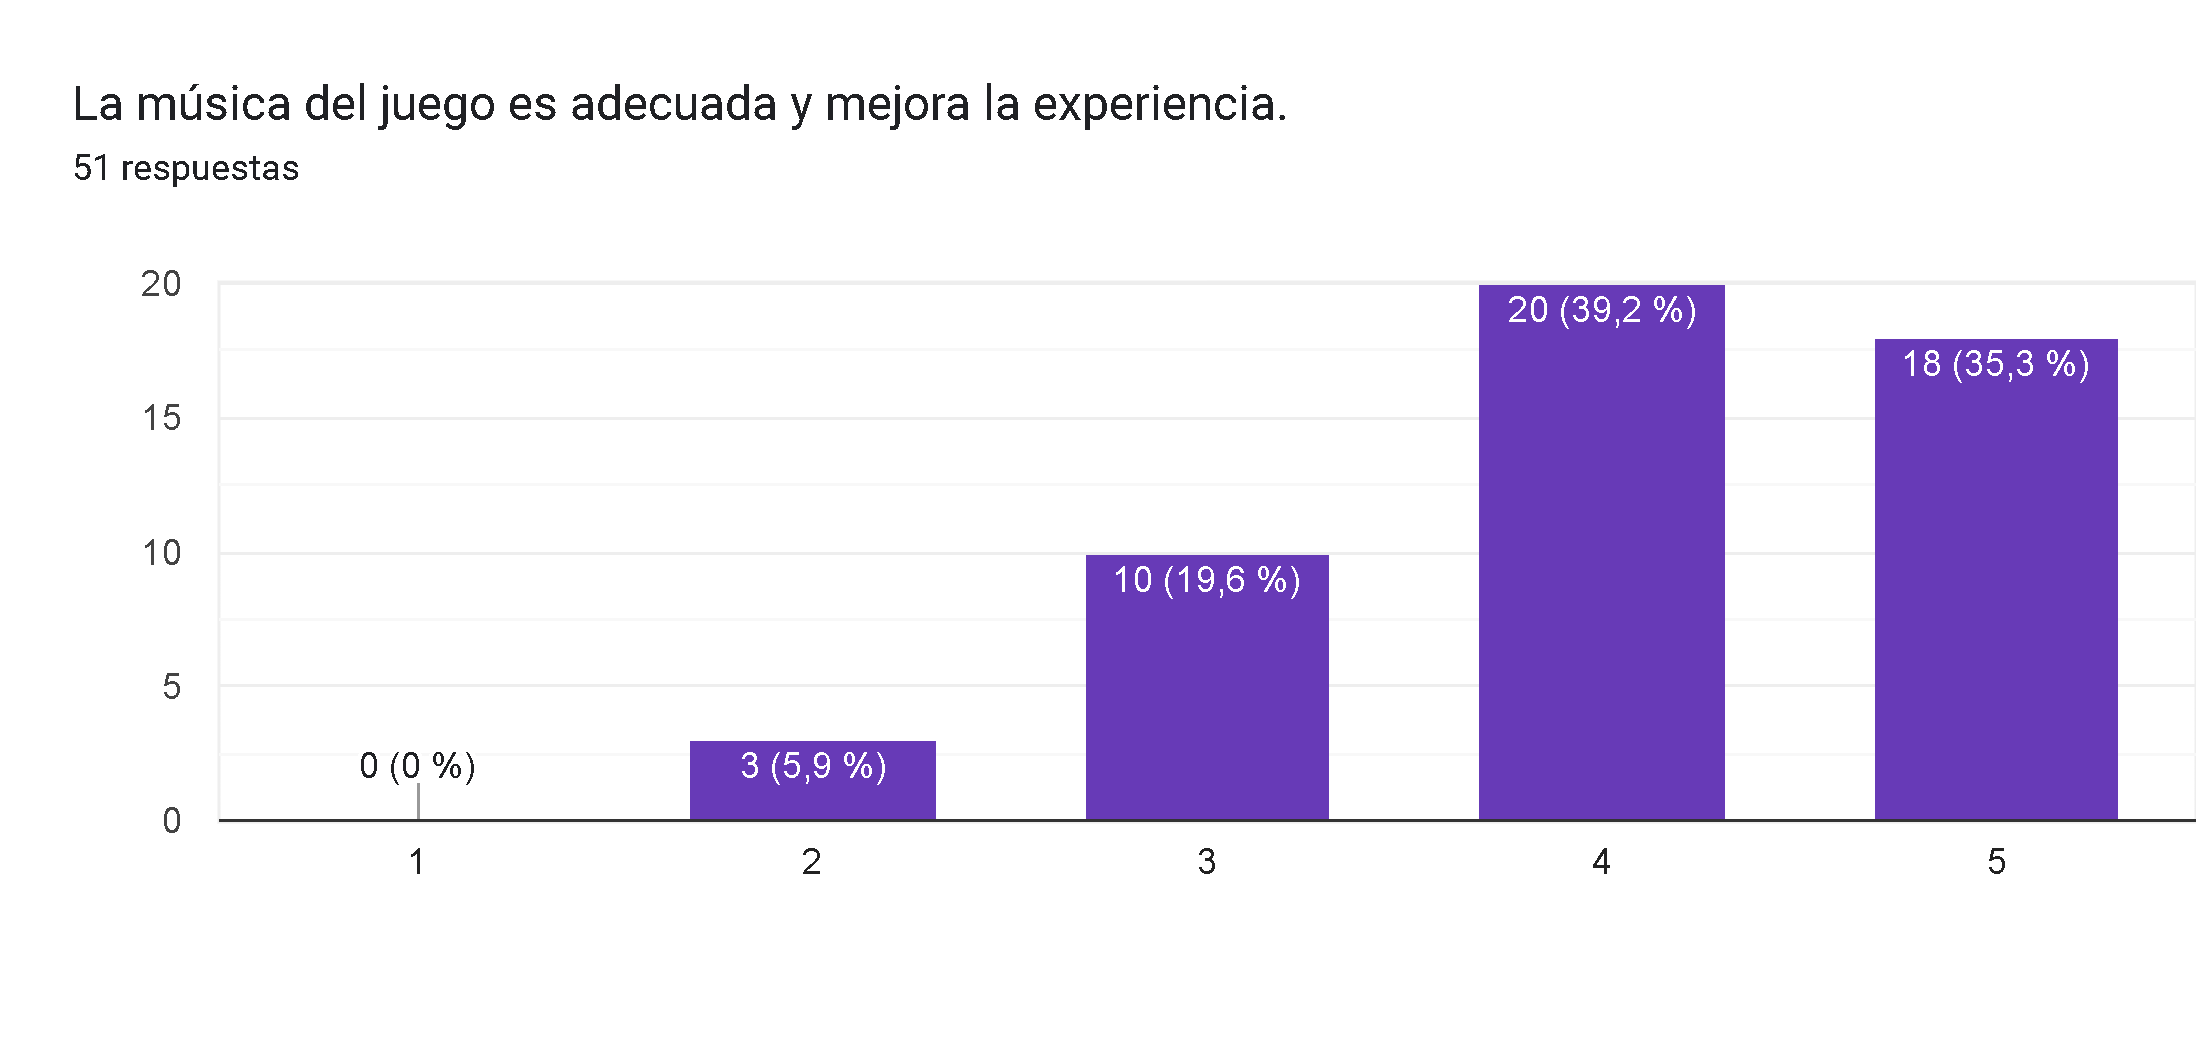
\includegraphics[width=0.7\linewidth]{Imagenes/mc5.png}
  \caption{Elaboración propia, Módulo mindset, Imagen de referencia sobre cuestionario de gamificación para el módulo mindset del juego sobre puzzles, ``La música del juego es adecuada y mejora la experiencia``}
  \label{fig:cuestionario5mindset}
\end{figure}



La pregunta ``El juego se ejecuta sin problemas de rendimiento (lag, caídas de FPS, etc.)`` obtuvo la mayor cantidad de respuestas en la opción 5, con un 41,2 \%. Esto indica que la mayoría de los usuarios experimenta un rendimiento sin problemas significativos.

\begin{figure}[H]
  \centering
  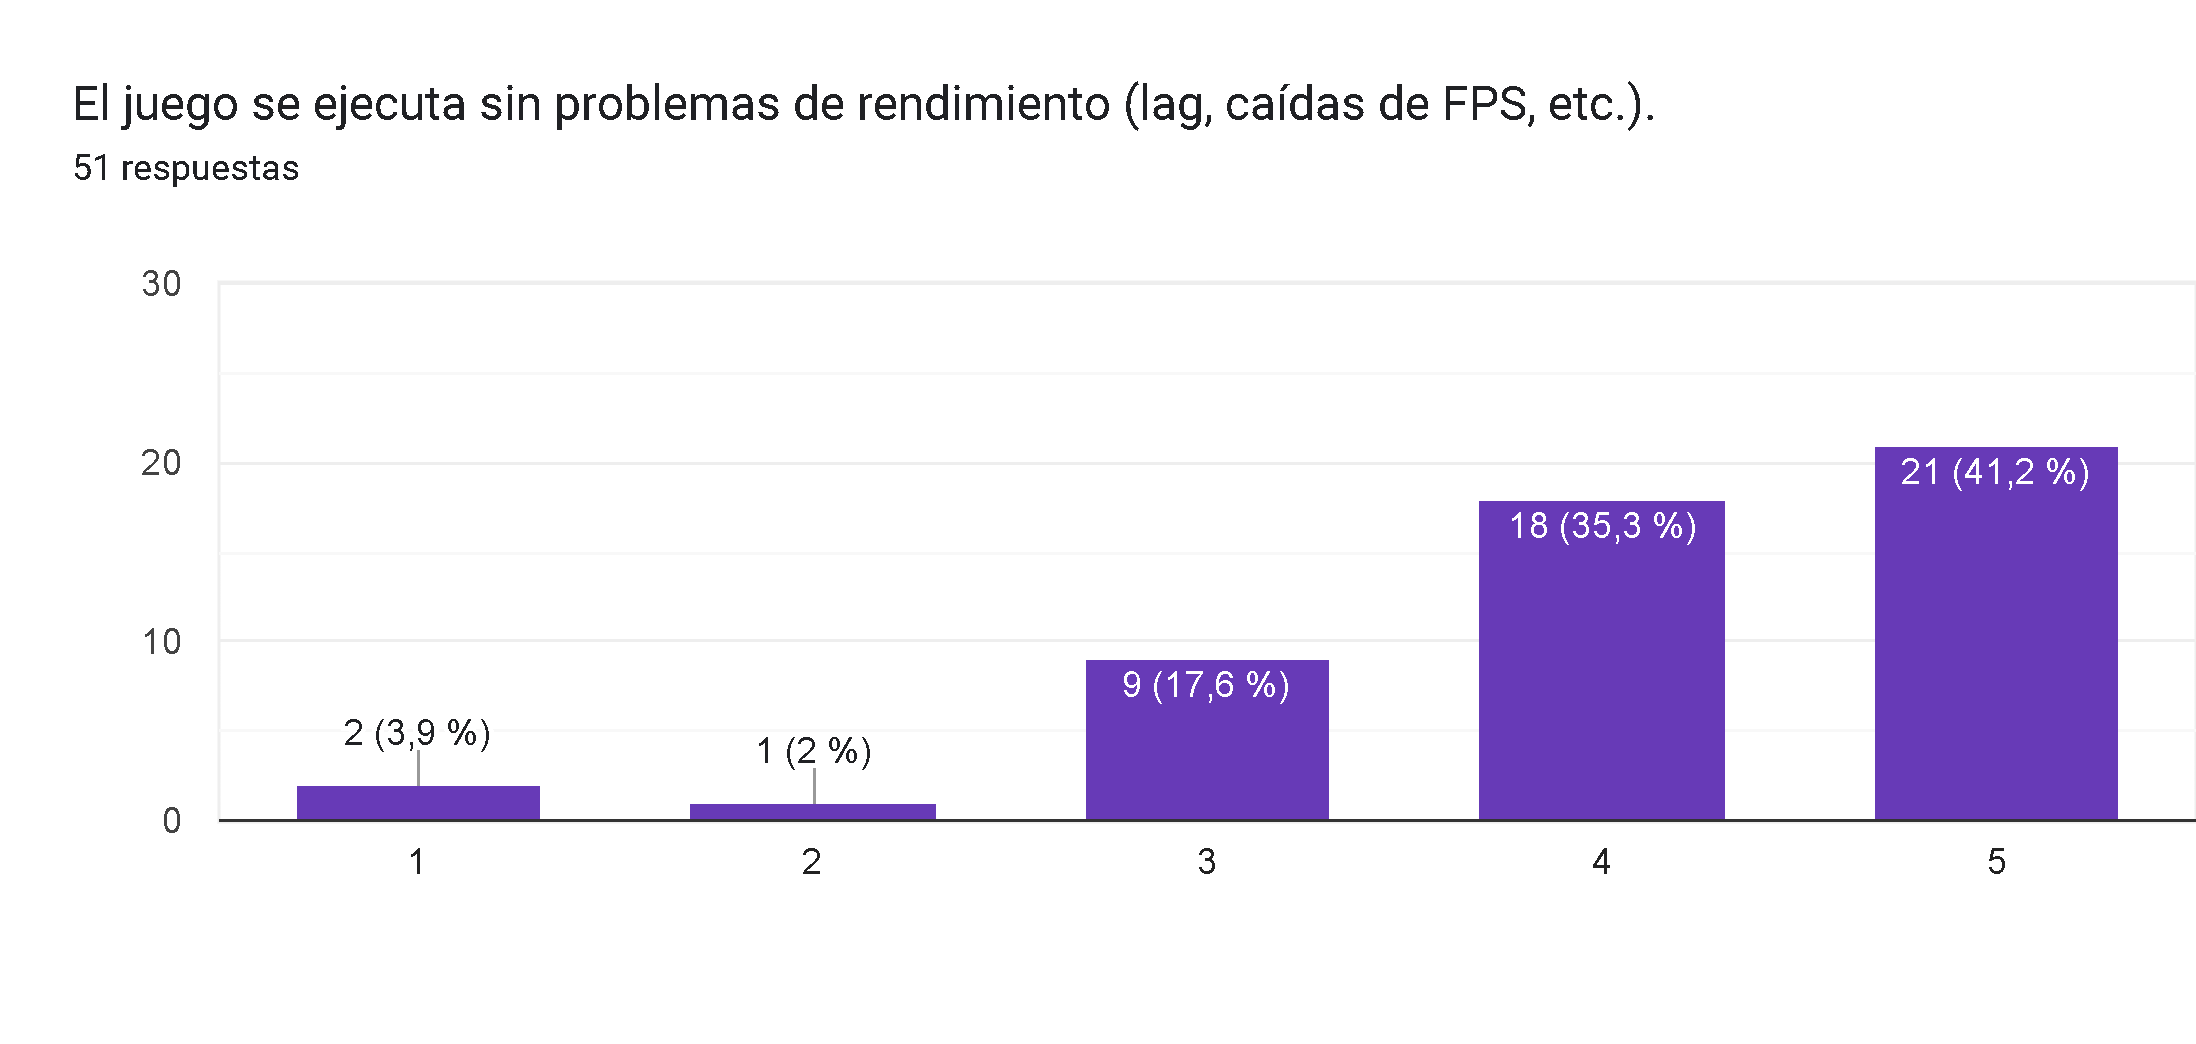
\includegraphics[width=0.7\linewidth]{Imagenes/mc6.png}
  \caption{Elaboración propia, Módulo mindset, Imagen de referencia sobre cuestionario de gamificación para el módulo mindset del juego sobre puzzles, ``El juego se ejecuta sin problemas de rendimiento (lag, caídas de FPS, etc.)``}
  \label{fig:cuestionario6mindset}
\end{figure}

La pregunta ``No he experimentado fallos técnicos o bugs importantes`` obtuvo la mayor cantidad de respuestas en la opción 4, con 25 respuestas. Esto sugiere que la mayoría de los usuarios no han experimentado fallos importantes, aunque aún hay algunos que podrían haber encontrado errores menores o bugs en el juego.

\begin{figure}[H]
  \centering
  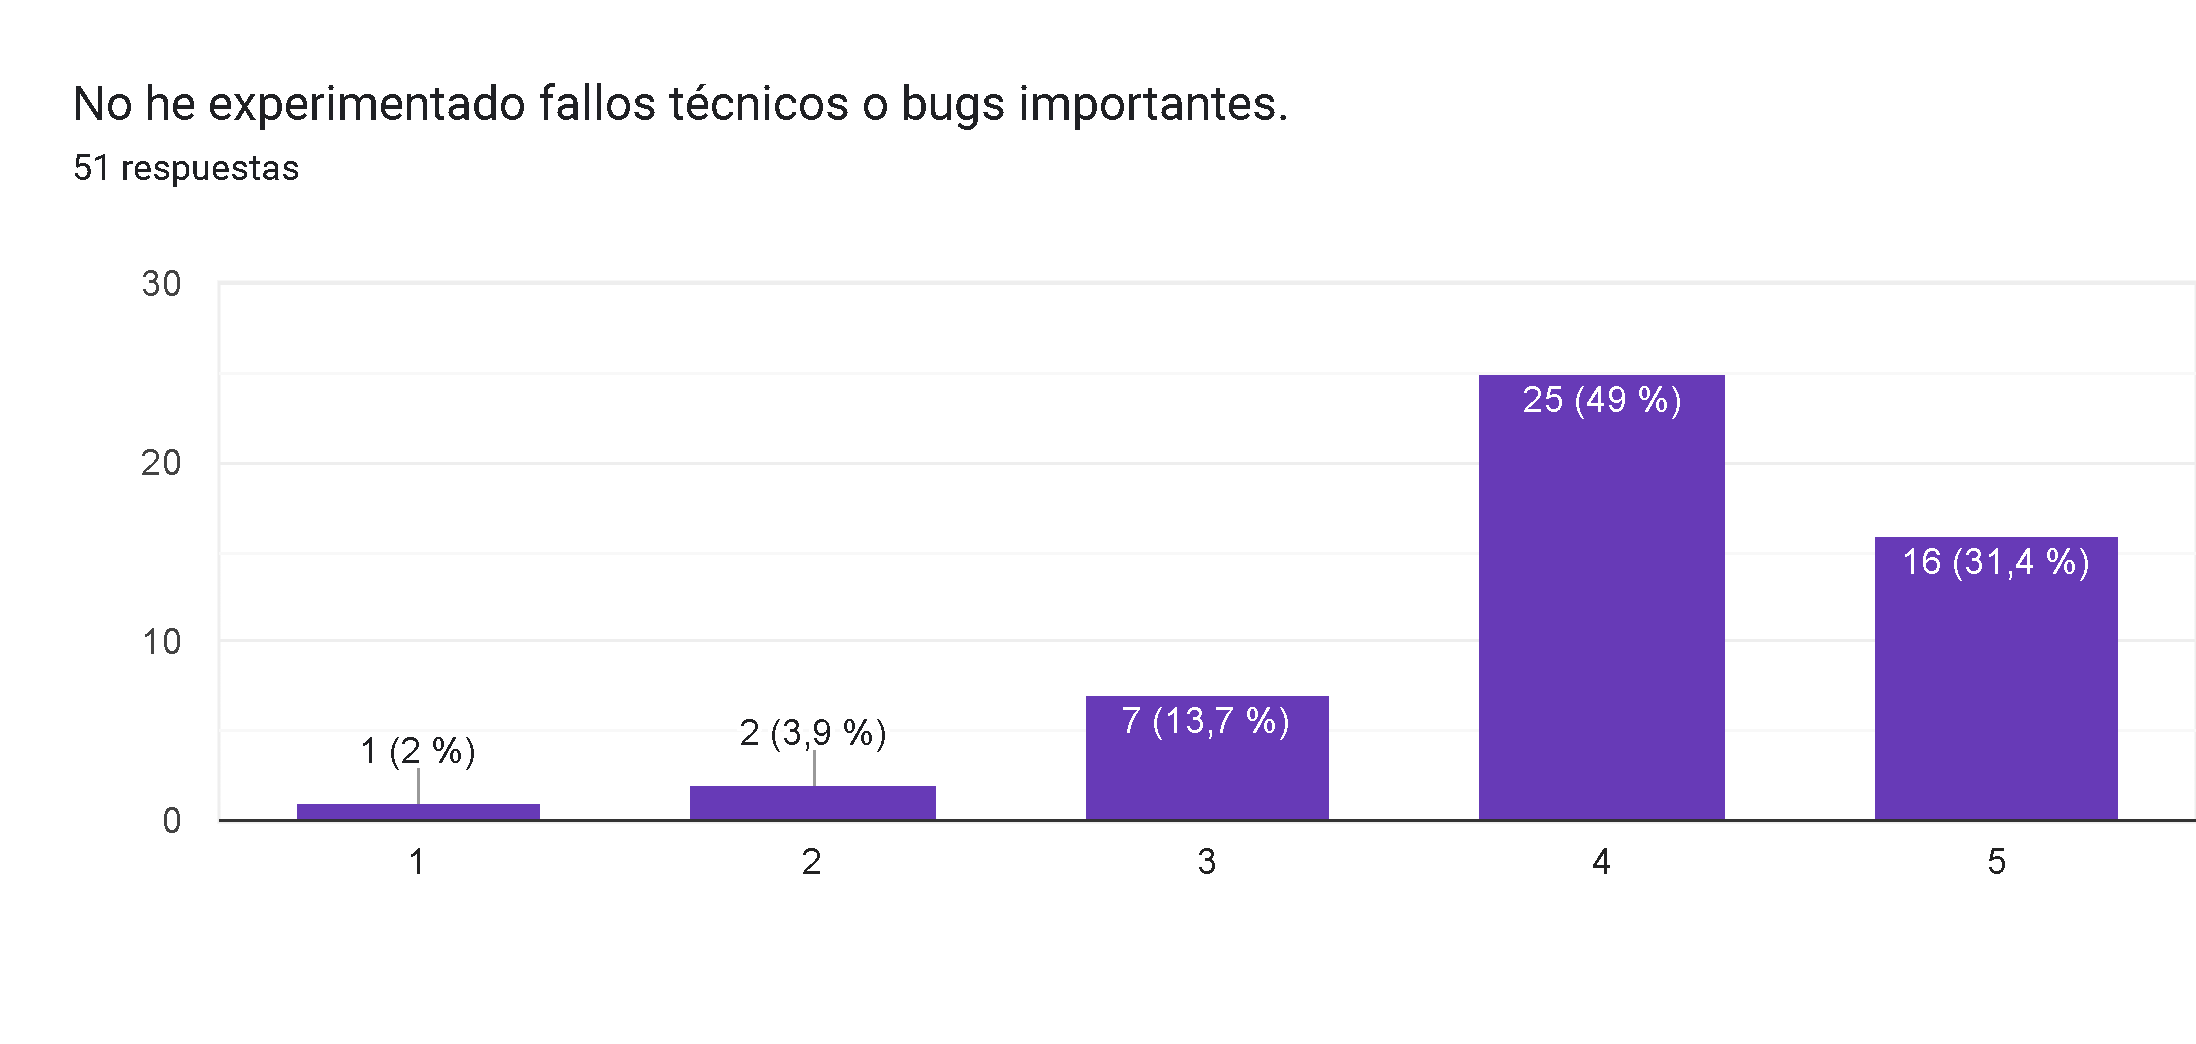
\includegraphics[width=0.7\linewidth]{Imagenes/mc7.png}
  \caption{Elaboración propia, Módulo mindset, Imagen de referencia sobre cuestionario de gamificación para el módulo mindset del juego sobre puzzles, ``No he experimentado fallos técnicos o bugs importantes``}
  \label{fig:cuestionario7mindset}
\end{figure}



La pregunta ``El juego me ha mantenido motivado para seguir jugando`` obtuvo la mayor cantidad de respuestas en la opción 5, con un 42 \%. Esto indica que la mayoría de los usuarios se sienten motivados para continuar jugando, aunque un porcentaje también respondió afirmativamente en la opción 4, con un 32 \%.

\begin{figure}[H]
  \centering
  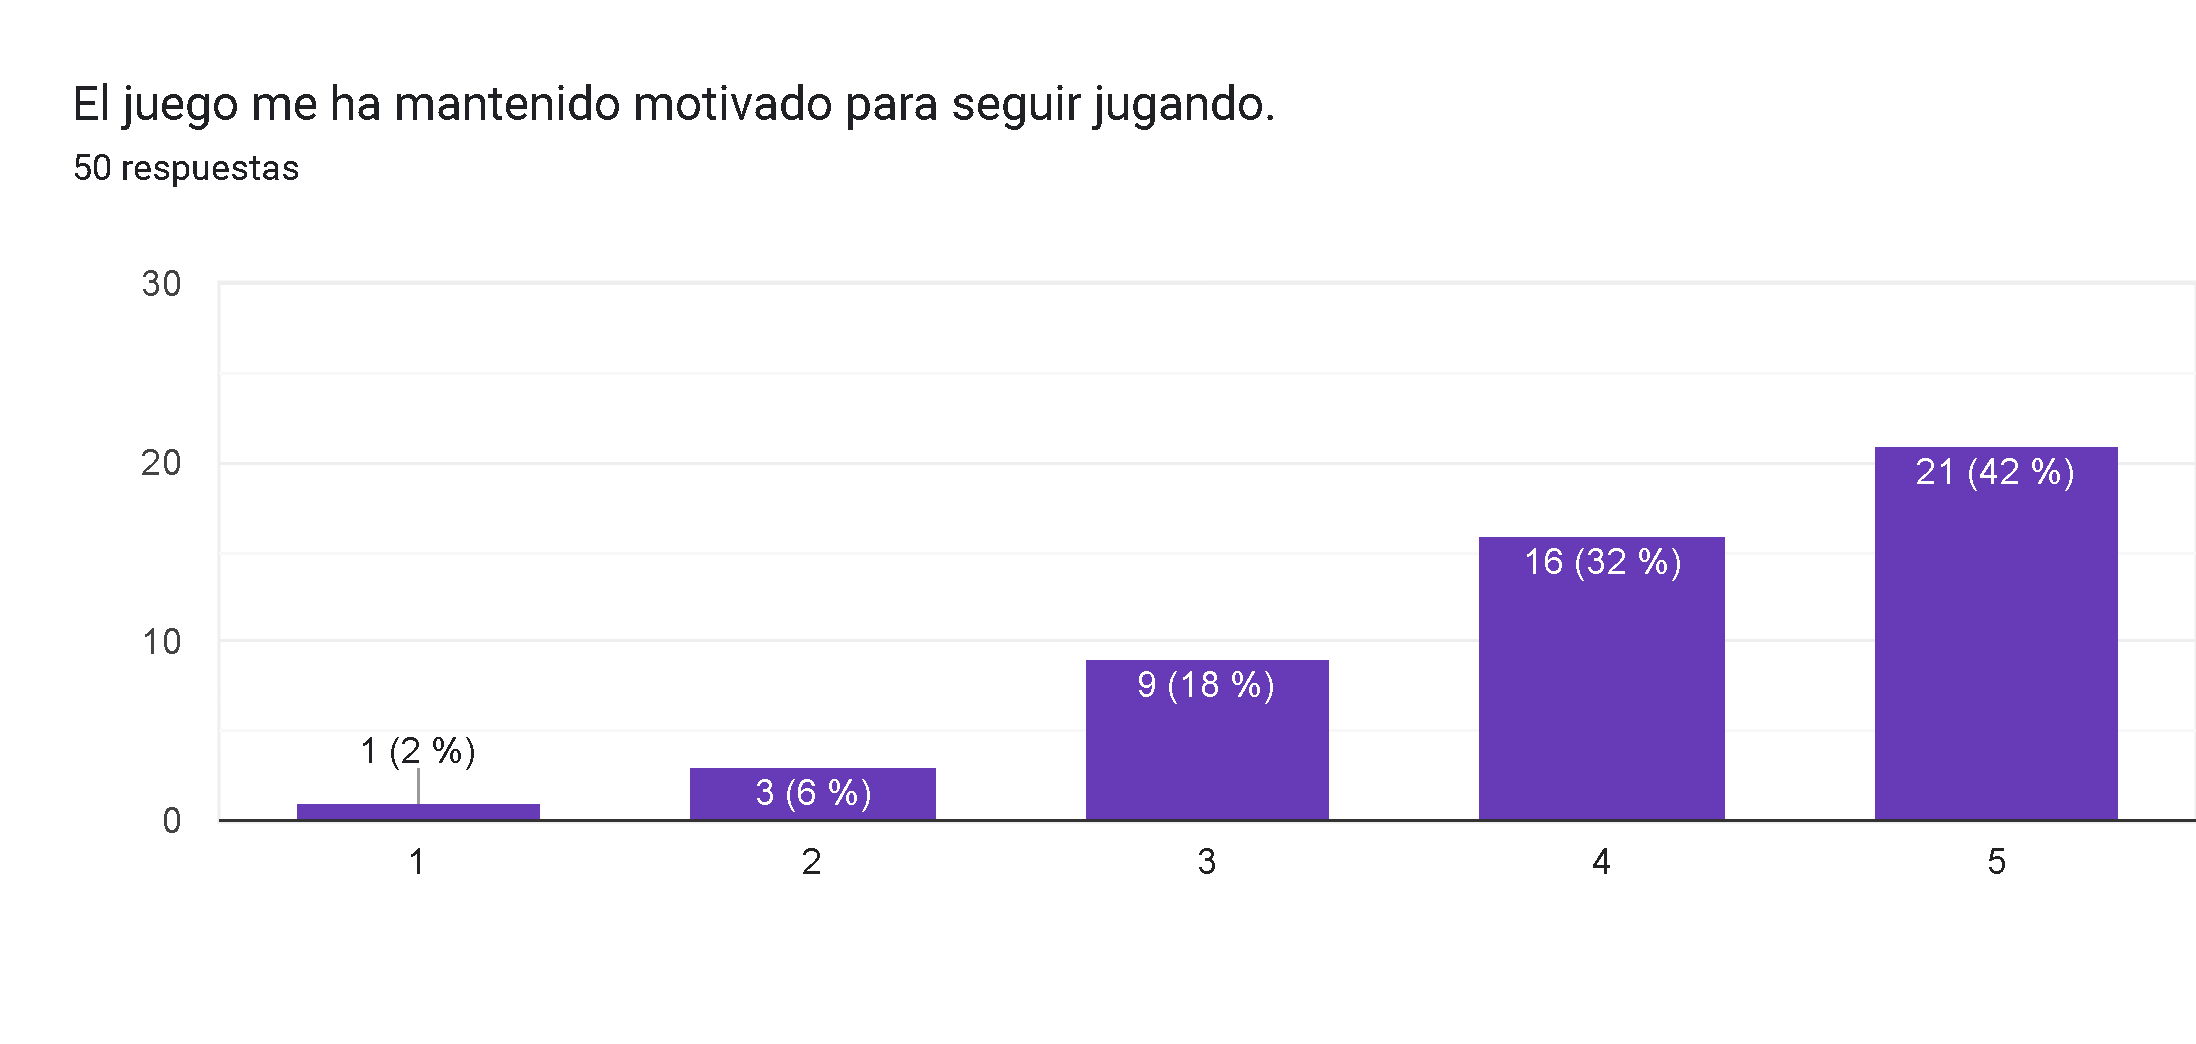
\includegraphics[width=0.7\linewidth]{Imagenes/mc8.png}
  \caption{Elaboración propia, Módulo mindset, Imagen de referencia sobre cuestionario de gamificación para el módulo mindset del juego sobre puzzles, ``El juego me ha mantenido motivado para seguir jugando``}
  \label{fig:cuestionario8mindset}
\end{figure}



La pregunta ``Me siento satisfecho con la experiencia general del juego`` obtuvo la mayor cantidad de respuestas en la opción 4, con un 42,9 \%. Esto indica que la mayoría de los usuarios están satisfechos con la experiencia general del juego, mientras que un porcentaje significativo también eligió la opción 5, con un 38,8 \%.

\begin{figure}[H]
  \centering
  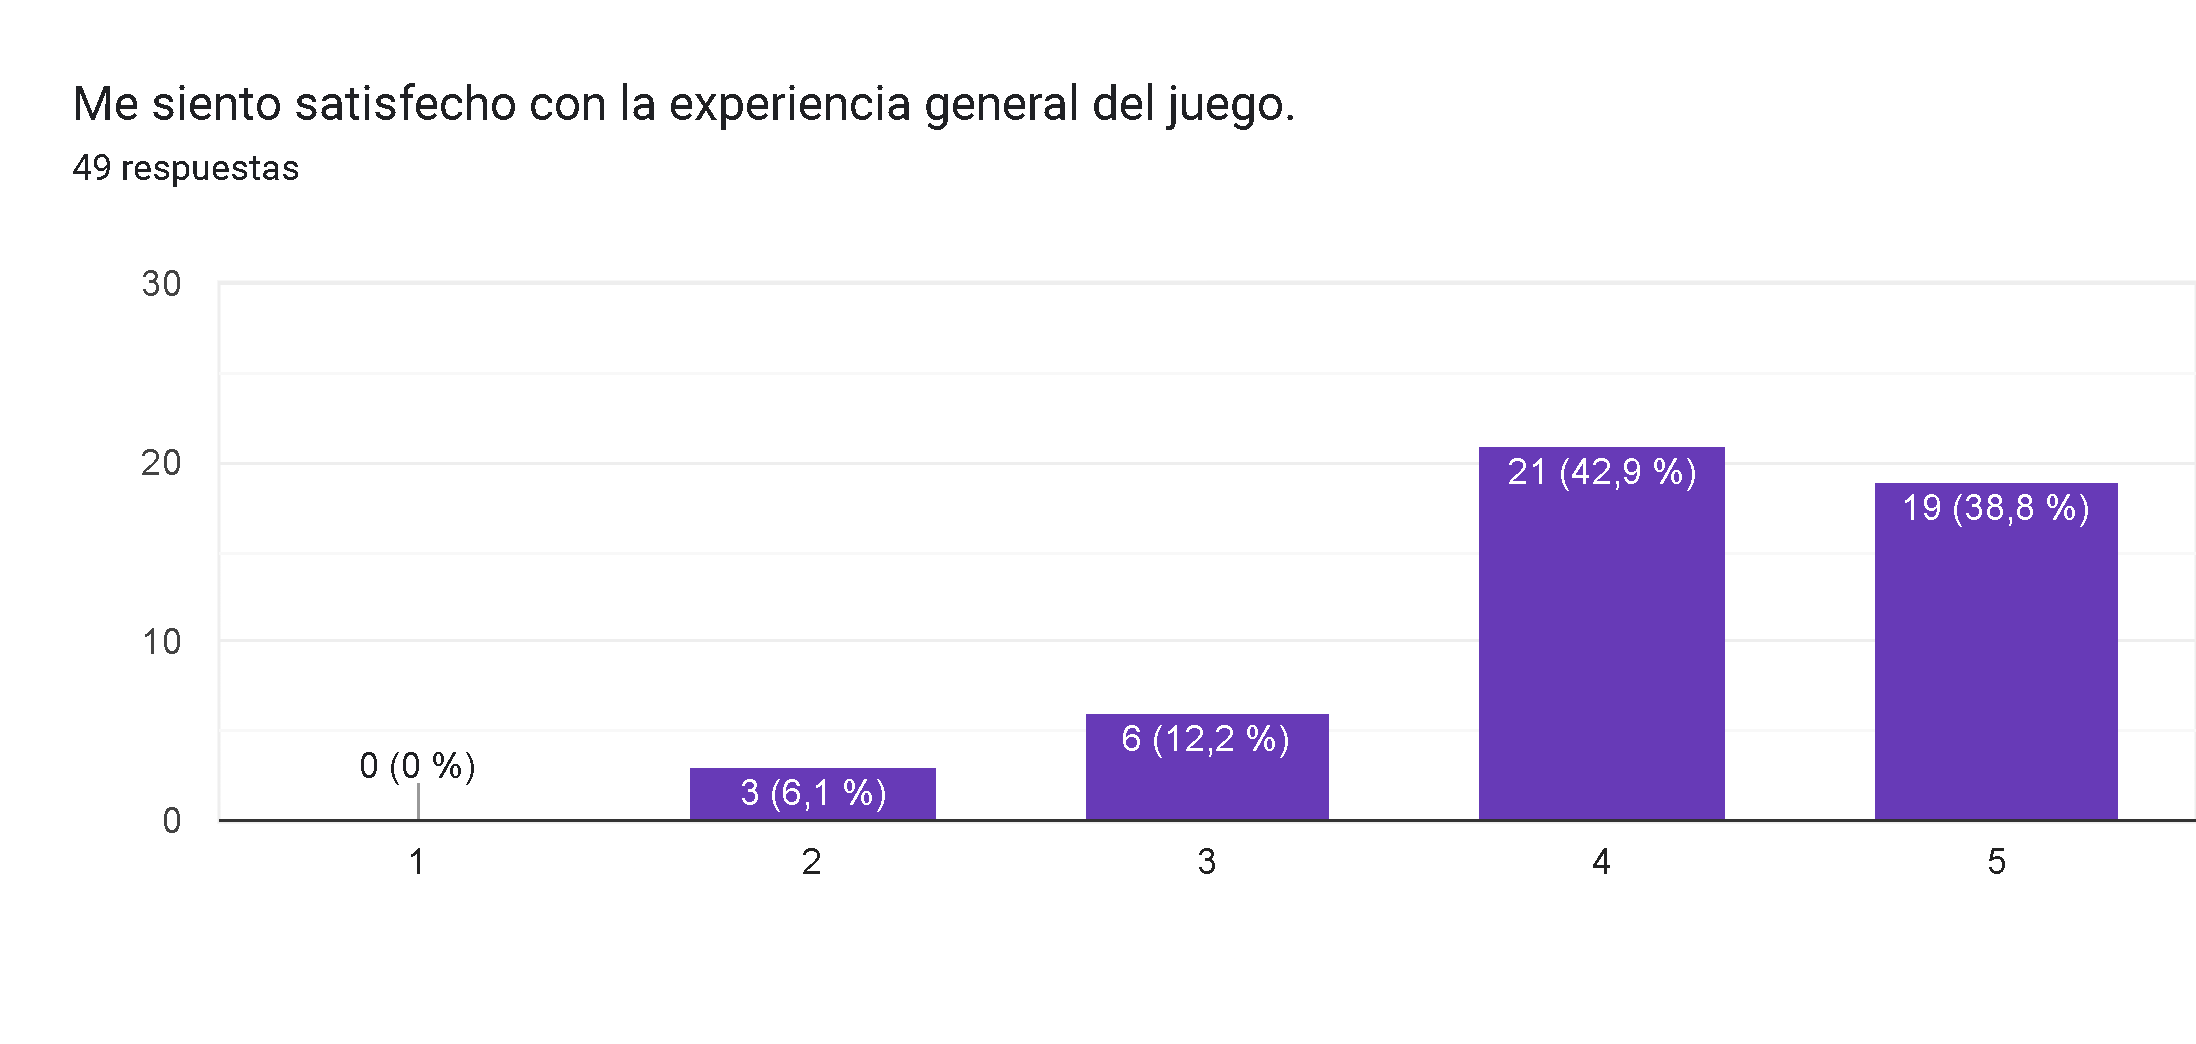
\includegraphics[width=0.7\linewidth]{Imagenes/mc9.png}
  \caption{Elaboración propia, Módulo mindset, Imagen de referencia sobre cuestionario de gamificación para el módulo mindset del juego sobre puzzles, ``Me siento satisfecho con la experiencia general del juego``}
  \label{fig:cuestionario9mindset}
\end{figure}



La pregunta ``Consideras que el juego es útil para el desarrollo de habilidades deductivas`` obtuvo la mayor cantidad de respuestas en la opción 5, con un 43,1 \%. Además, un 37,3 \% eligió la opción 4, lo que sugiere que una mayoría considera que el juego es útil para desarrollar habilidades deductivas, aunque también hay una proporción significativa que tiene una opinión positiva, pero no tan rotunda.

\begin{figure}[H]
  \centering
  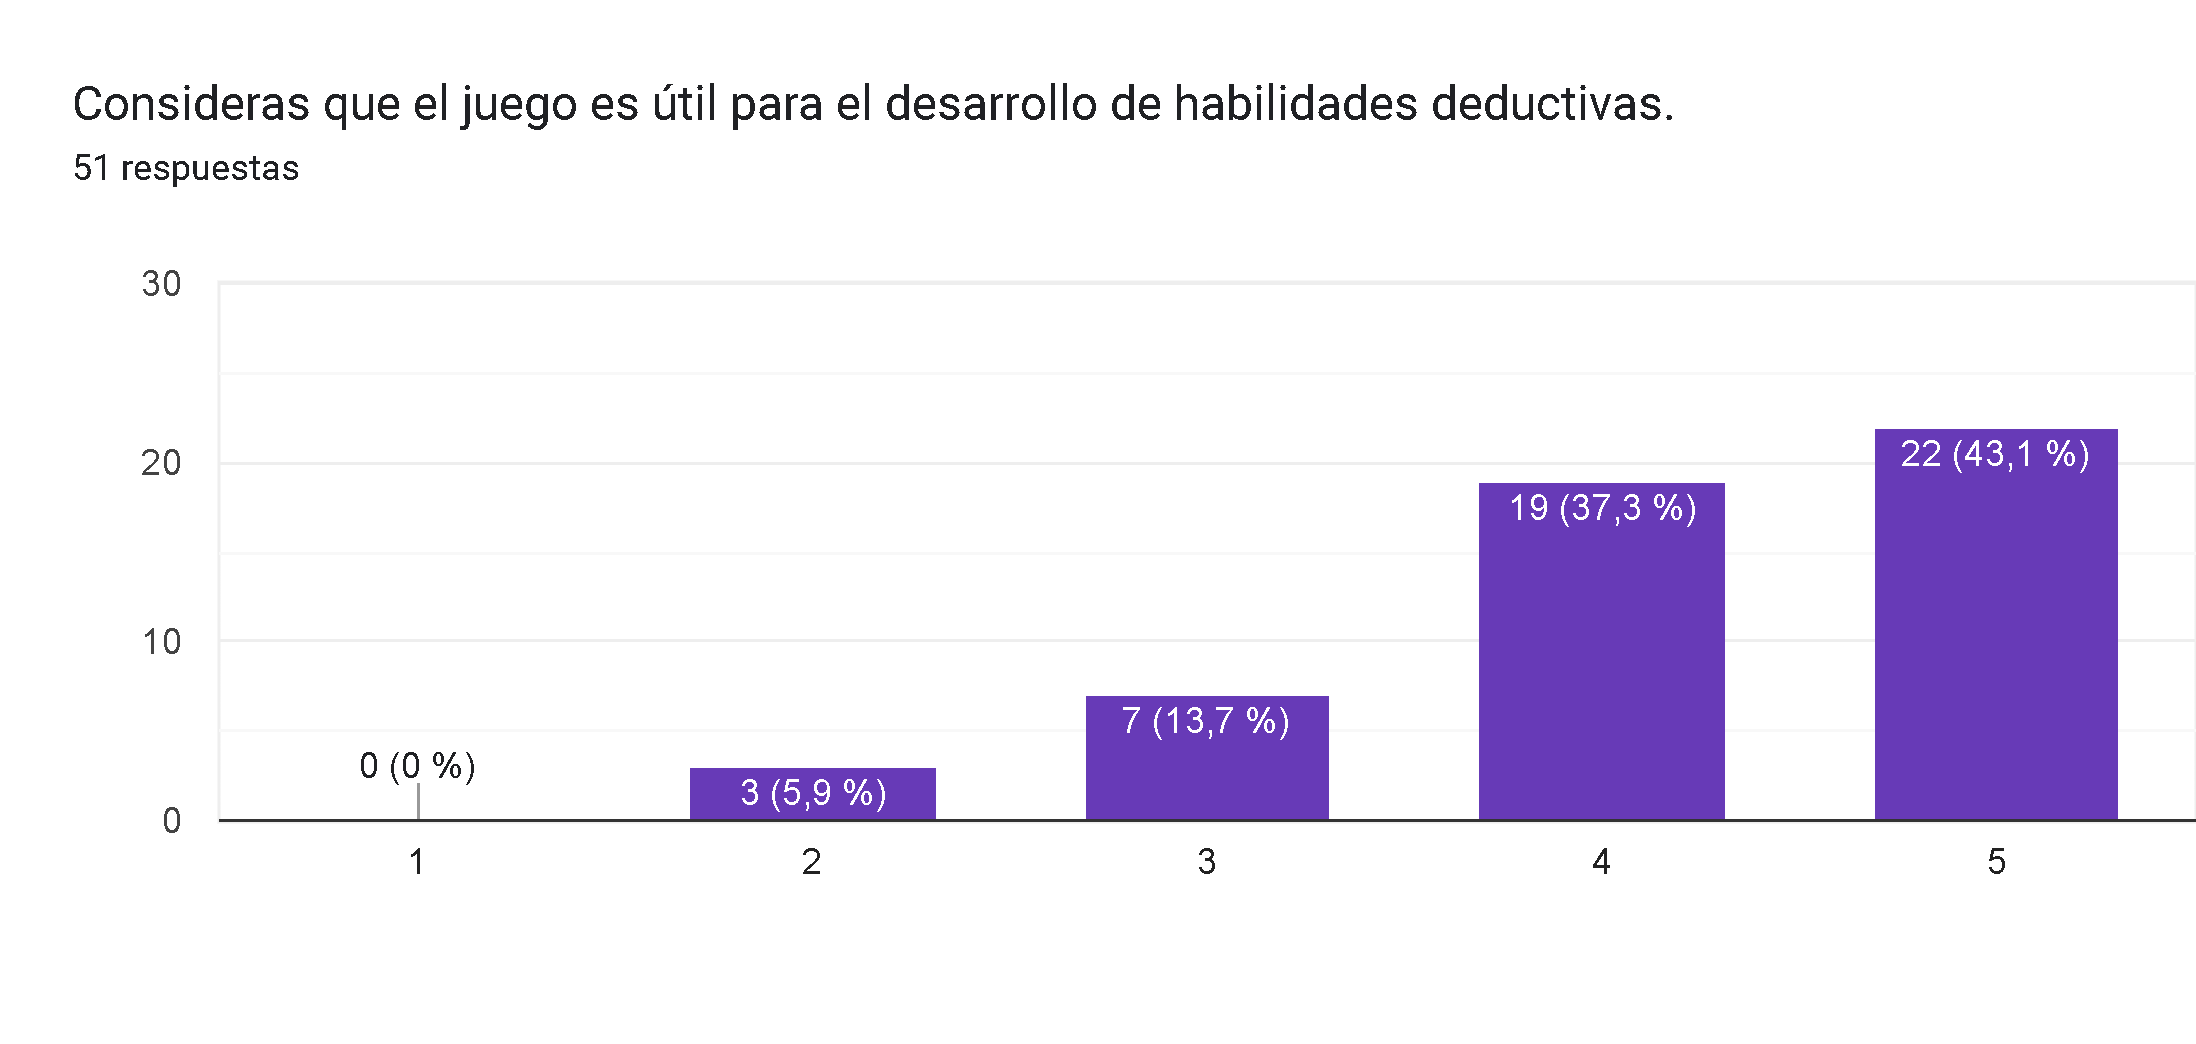
\includegraphics[width=0.7\linewidth]{Imagenes/mc10.png}
  \caption{Elaboración propia, Módulo mindset, Imagen de referencia sobre cuestionario de gamificación para el módulo mindset del juego sobre puzzles, ``Consideras que el juego es útil para el desarrollo de habilidades deductivas``}
  \label{fig:cuestionario10mindset}
\end{figure}

La pregunta ``Consideras que el juego es útil para el desarrollo de la resiliencia y el cómo afrontar los desafíos`` obtuvo la mayor cantidad de respuestas en la opción 4, con un 50 \%. Esto indica que la mayoría de los usuarios considera que el juego tiene un impacto positivo en el desarrollo de la resiliencia y la capacidad para afrontar los desafíos.

\begin{figure}[H]
  \centering
  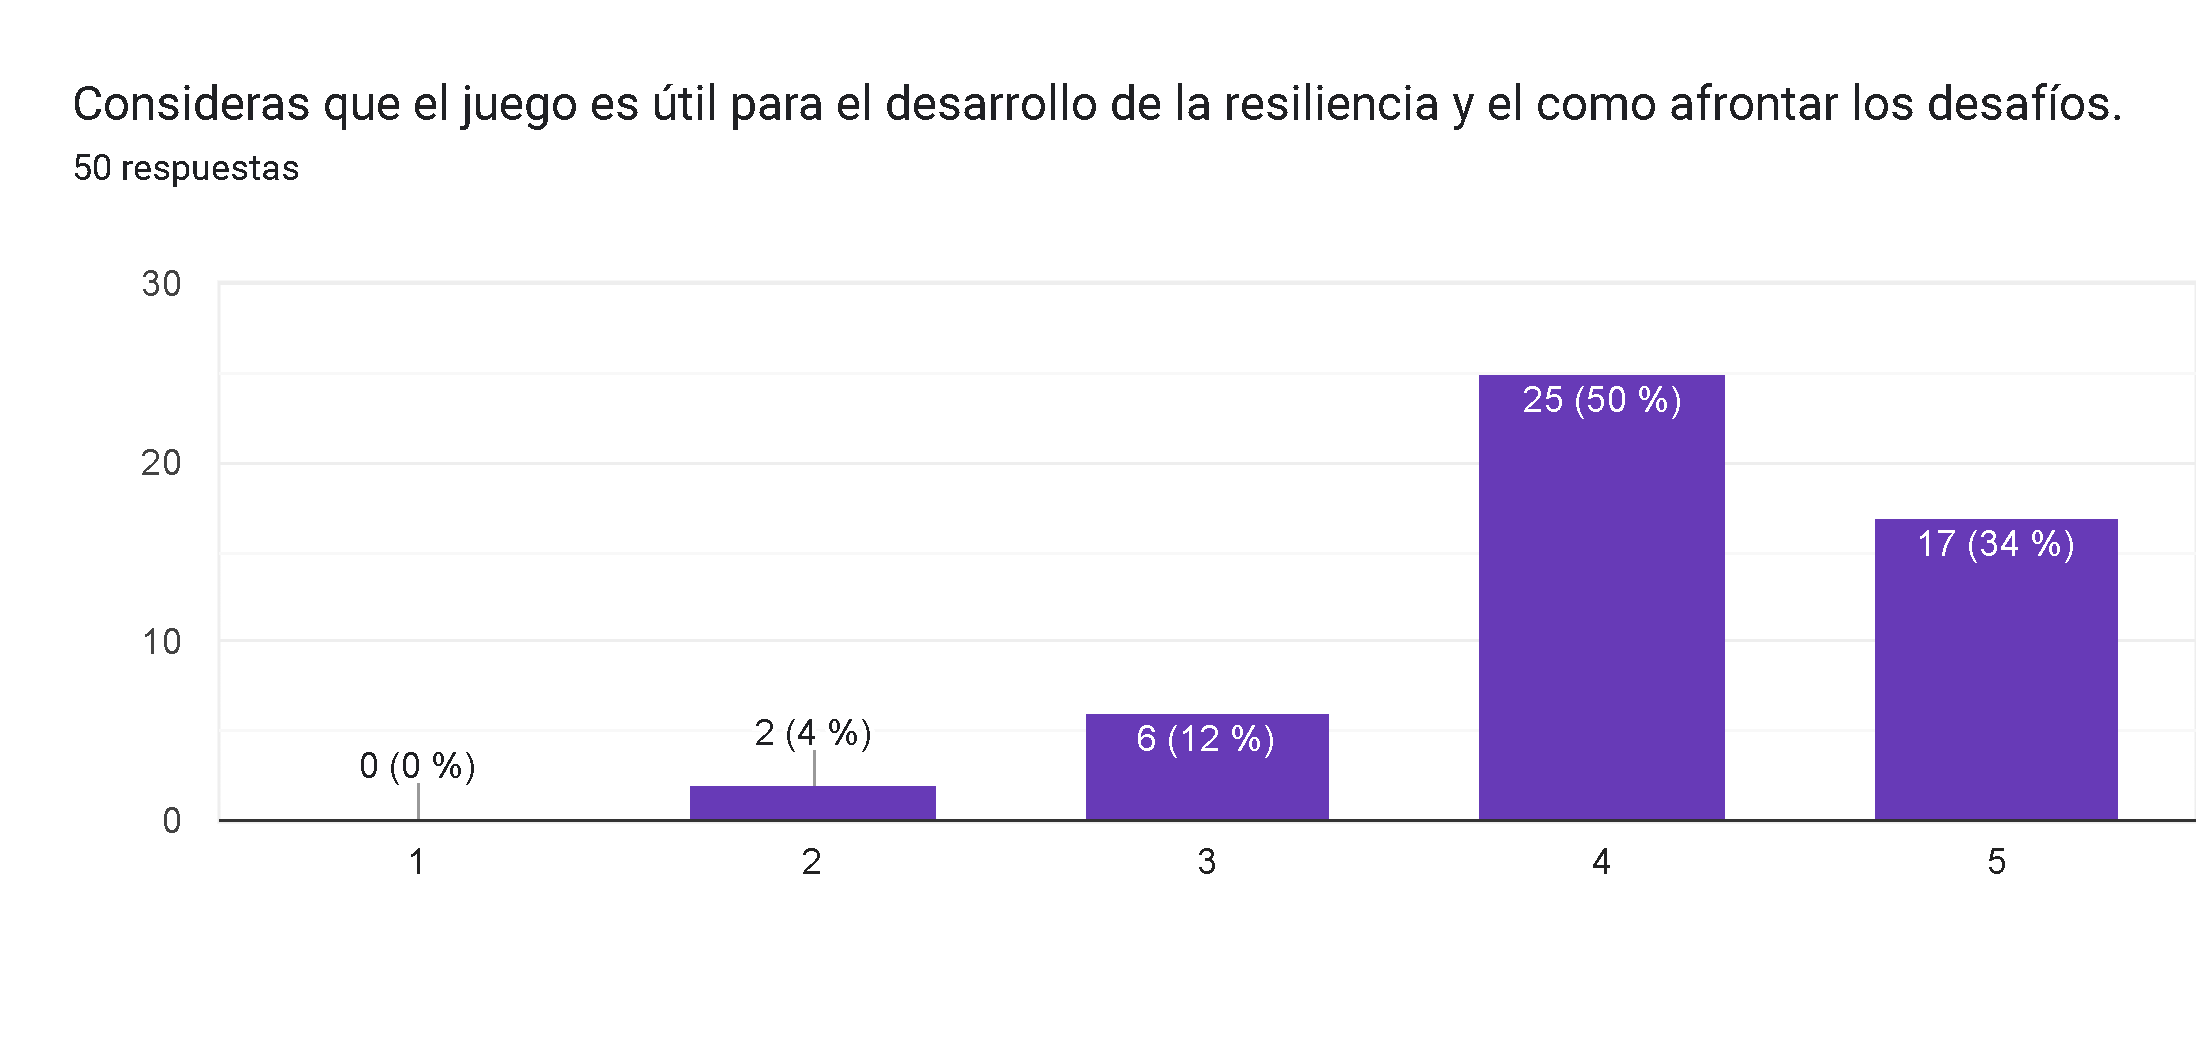
\includegraphics[width=0.7\linewidth]{Imagenes/mc11.png}
  \caption{Elaboración propia, Módulo mindset, Imagen de referencia sobre cuestionario de gamificación para el módulo mindset del juego sobre puzzles, ``Consideras que el juego es útil para el desarrollo de la resiliencia y el cómo afrontar los desafíos``}
  \label{fig:cuestionario11mindset}
\end{figure}


\section{Cuestionario sobre pruebas de usabilidad heurísticas de Nielsen para plataforma gamificada sobre módulos Mindset y Fitness}
La pregunta ``¿La plataforma te mantuvo informado sobre el progreso del juego o el estado actual, como tiempos de carga o indicadores de avance en los ejercicios de fitness y mindset?'' obtuvo la mayor cantidad de respuestas en la opción 5, con un 50\%. Esto sugiere que la mayoría de los usuarios se sintieron informados sobre su progreso durante el juego, apreciando los indicadores de avance y tiempos de carga. Además, un 30\% de los usuarios seleccionaron la opción 3, lo que indica que una parte también percibió cierta falta de información o detalles sobre el estado del juego. Un 20\% de los usuarios respondió en la opción 2, lo que podría indicar que algunos encontraron insuficiente la información proporcionada por la plataforma.

\begin{figure}[H]
  \centering
  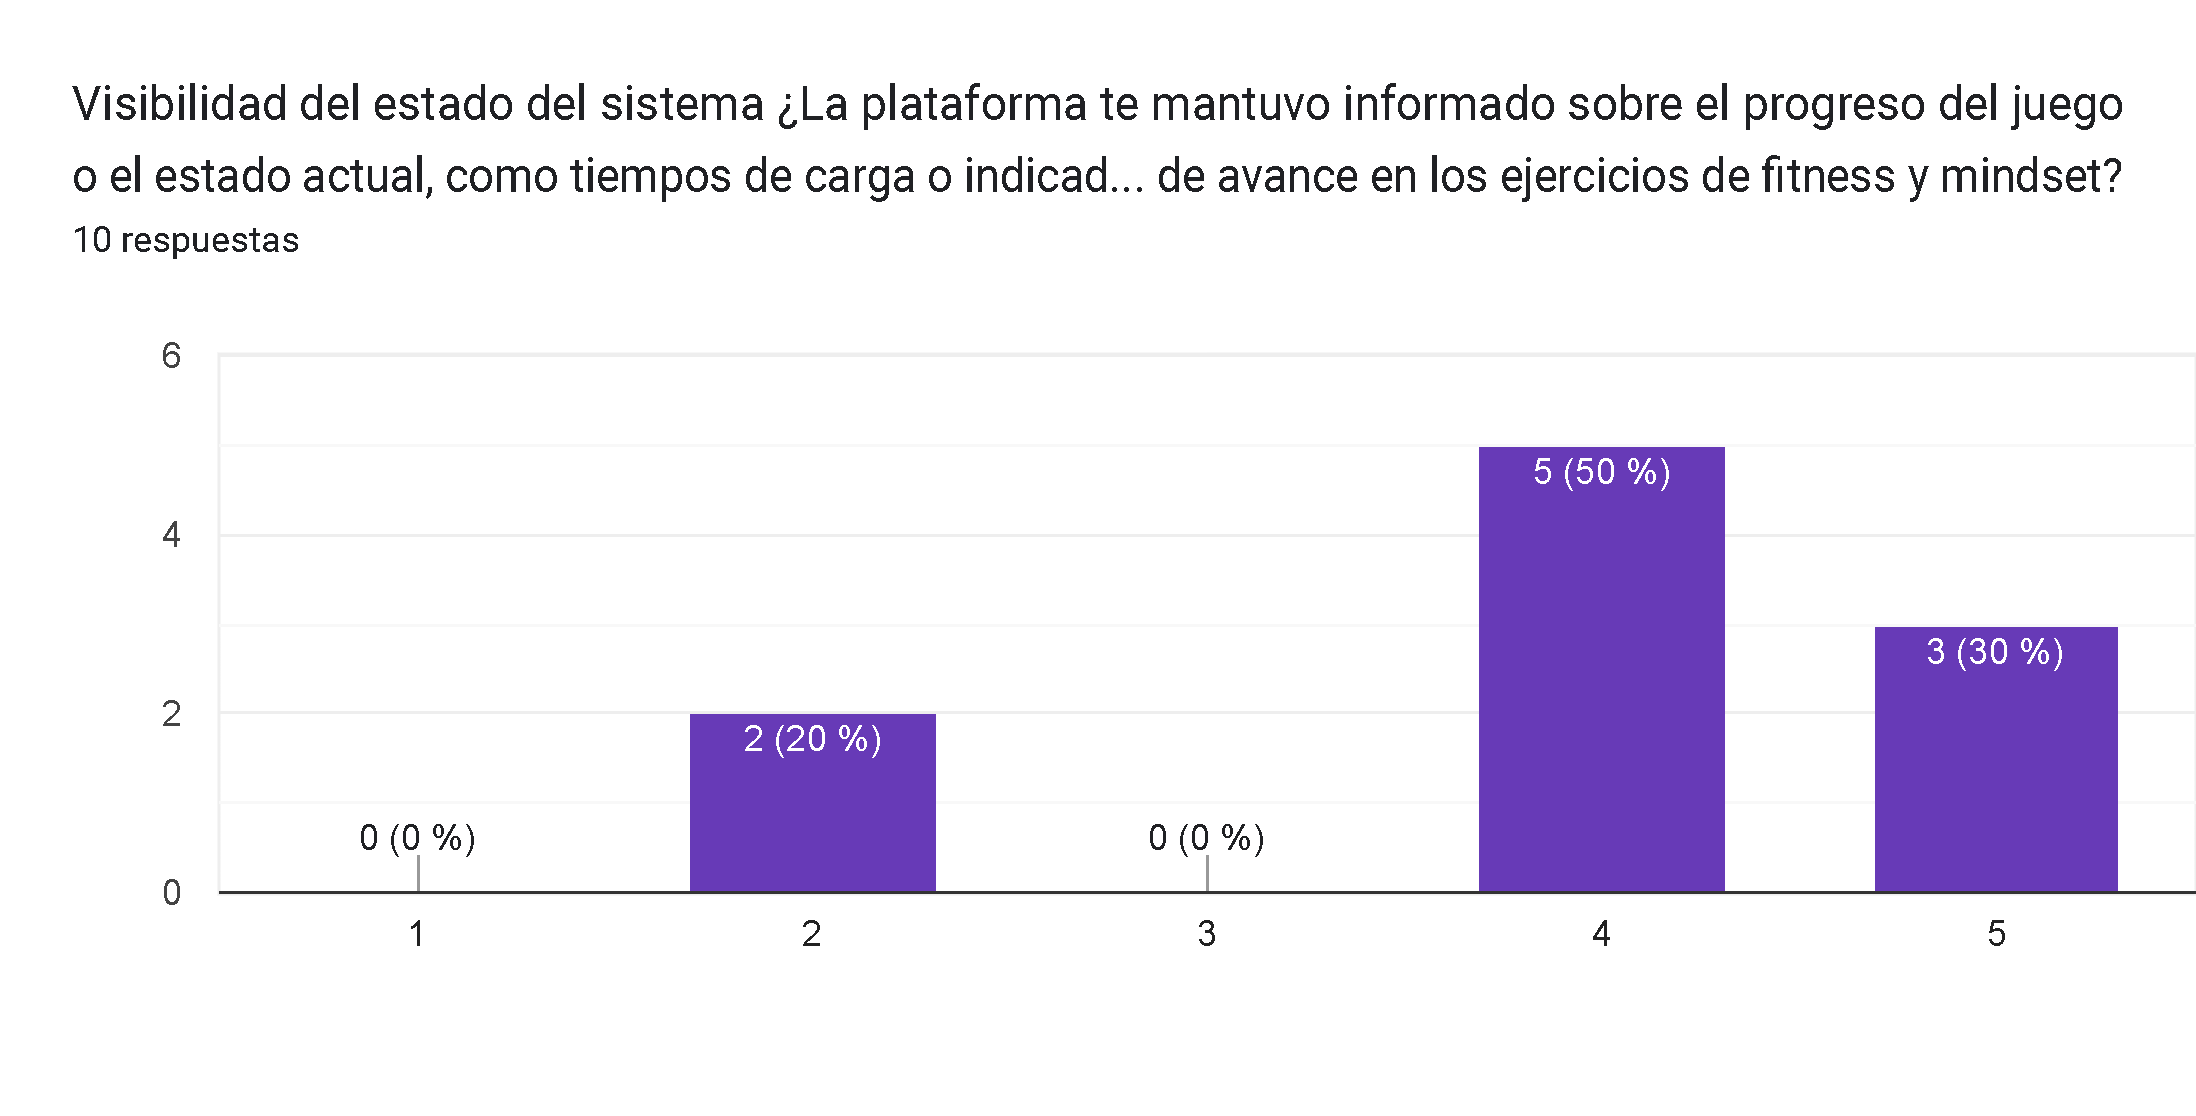
\includegraphics[width=0.7\linewidth]{Imagenes/Nc1.png}
  \caption{Elaboración propia, Imagen de referencia de cuestionario sobre pruebas de usabilidad heurísticas de Nielsen para plataforma gamificada sobre módulos Mindset y Fitness, `¿La plataforma te mantuvo informado sobre el progreso del juego o el estado actual, como tiempos de carga o indicadores de avance en los ejercicios de fitness y mindset?'}

  \label{fig:cuestionario1nielsen}
\end{figure}

La pregunta ``¿Los términos utilizados en los juegos (por ejemplo, instrucciones de ejercicios) fueron fáciles de entender y reflejaron el lenguaje que esperas en estos contextos?'' obtuvo la mayor cantidad de respuestas en la opción 5, con un 50\%. Esto indica que la mayoría de los usuarios encontraron los términos utilizados en el juego claros y apropiados para el contexto. Además, un 30\% de los usuarios seleccionaron la opción 3, lo que sugiere que algunos usuarios consideraron que los términos eran comprensibles, pero podrían mejorarse. Un 20\% de los usuarios eligió la opción 2, lo que podría señalar que algunos encontraron dificultad con el lenguaje utilizado en las instrucciones o el contenido del juego.

\begin{figure}[H]
  \centering
  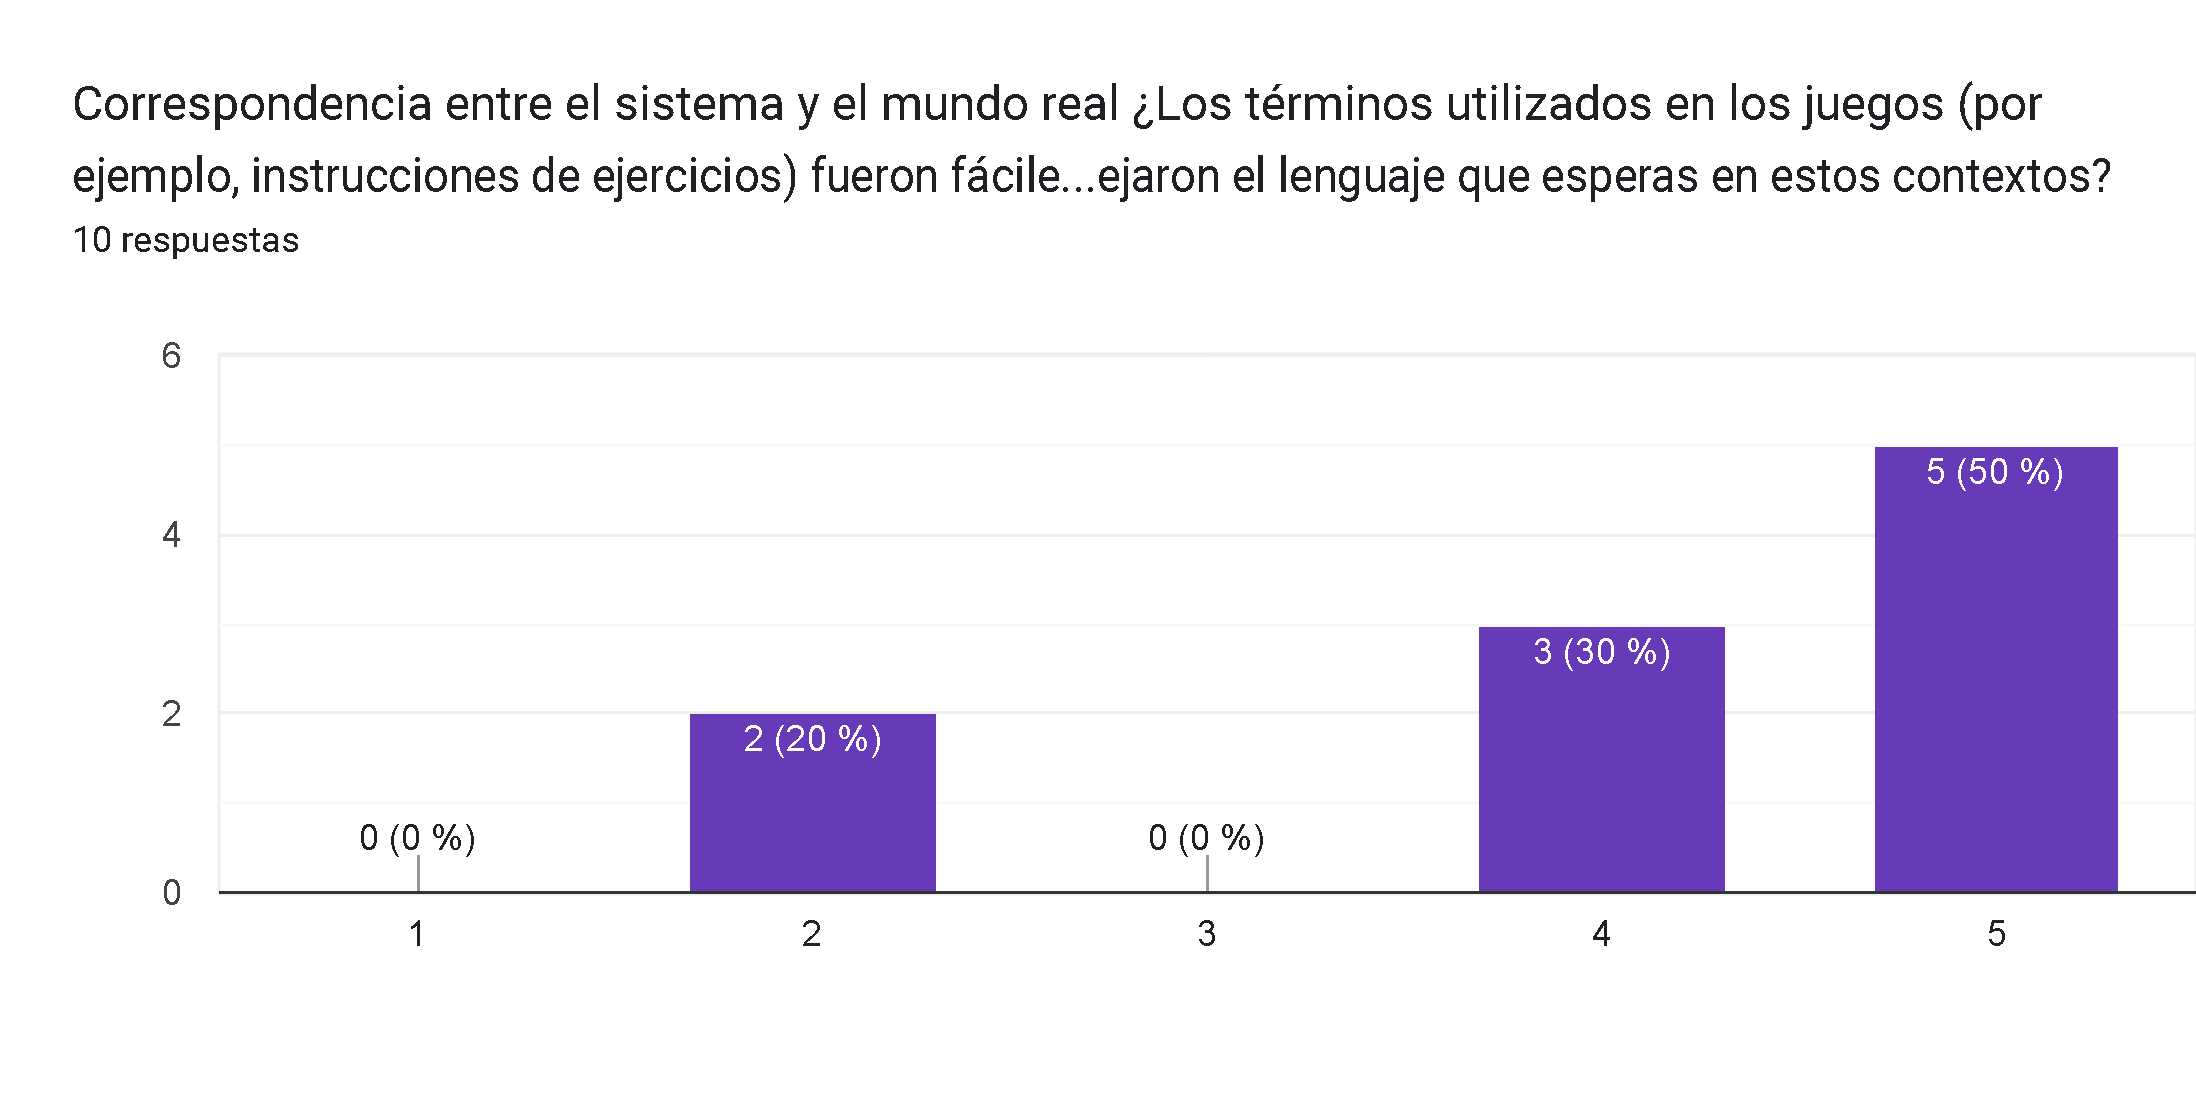
\includegraphics[width=0.7\linewidth]{Imagenes/Nc2.png}
  \caption{Elaboración propia, Imagen de referencia de cuestionario sobre pruebas de usabilidad heurísticas de Nielsen para plataforma gamificada sobre módulos Mindset y Fitness, `¿Los términos utilizados en los juegos (por ejemplo, instrucciones de ejercicios) fueron fáciles de entender y reflejaron el lenguaje que esperas en estos contextos?'}

  \label{fig:cuestionario2nielsen}
\end{figure}

La pregunta ``¿Pudiste salir o reiniciar los juegos de fitness y mindset fácilmente si cometiste un error o deseabas volver a intentarlo?'' obtuvo la mayor cantidad de respuestas en la opción 5, con un 50\%. Esto indica que la mayoría de los usuarios consideraron que la opción para reiniciar o salir del juego estaba fácilmente accesible y funcionaba correctamente. Un 30\% de los usuarios seleccionaron la opción 3, lo que sugiere que algunos encontraron la opción razonablemente accesible, aunque podrían haber experimentado alguna dificultad menor. Un 20\% eligió la opción 2, lo que sugiere que una pequeña parte de los usuarios tuvo dificultades para reiniciar o salir del juego de manera eficiente.

\begin{figure}[H]
  \centering
  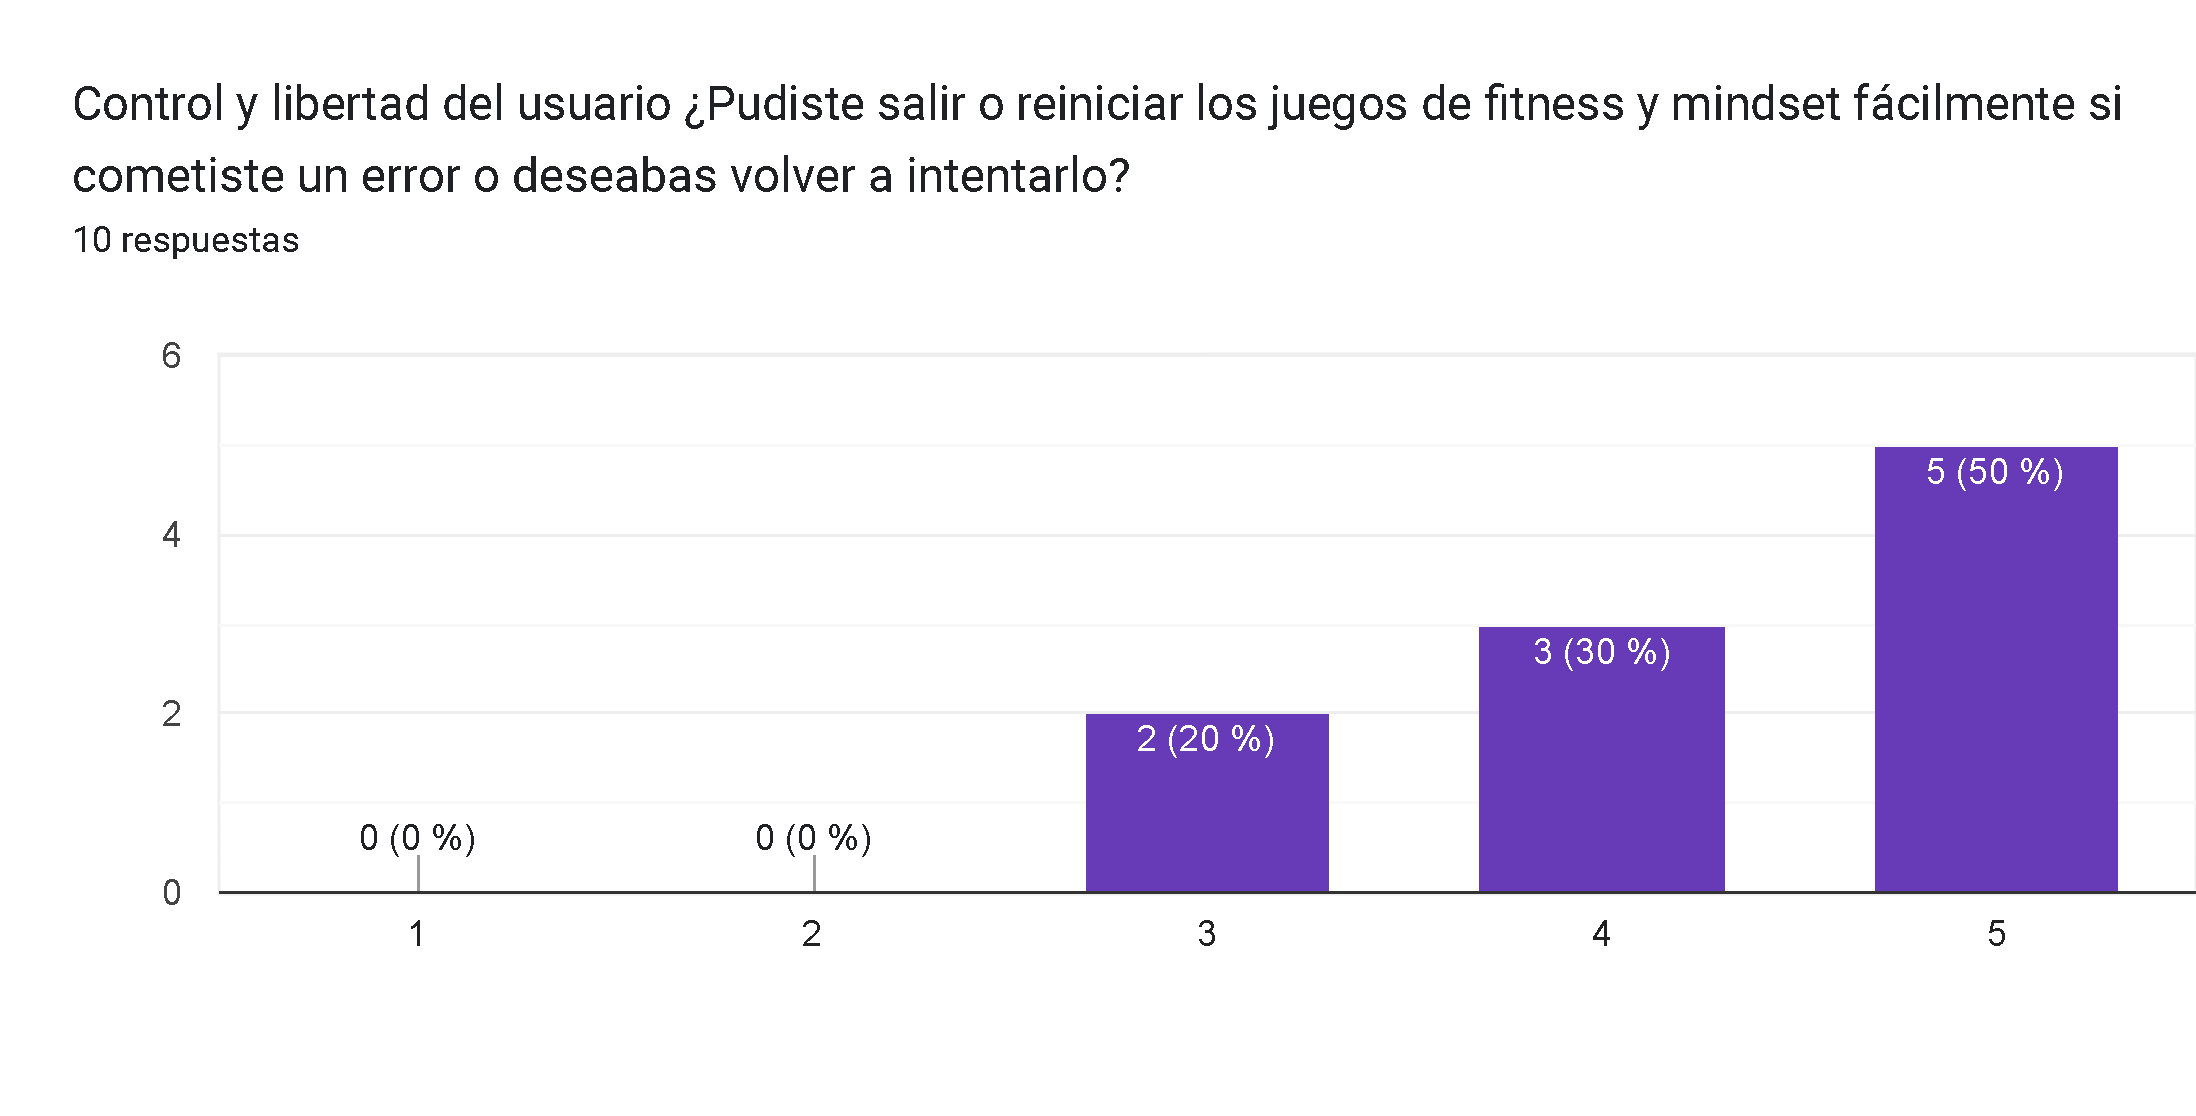
\includegraphics[width=0.7\linewidth]{Imagenes/Nc3.png}
  \caption{Elaboración propia, Imagen de referencia de cuestionario sobre pruebas de usabilidad heurísticas de Nielsen para plataforma gamificada sobre módulos Mindset y Fitness, `¿Pudiste salir o reiniciar los juegos de fitness y mindset fácilmente si cometiste un error o deseabas volver a intentarlo?'}

  \label{fig:cuestionario3nielsen}
\end{figure}

La pregunta ``¿Notaste alguna inconsistencia en la interfaz o en las acciones entre los diferentes juegos de fitness y mindset?'' obtuvo la mayor cantidad de respuestas en la opción 5, con un 50\%. Esto sugiere que la mayoría de los usuarios no notaron inconsistencias significativas entre los juegos de fitness y mindset. Un 30\% de los usuarios eligió la opción 3, lo que indica que algunos podrían haber percibido leves inconsistencias, pero estas no fueron lo suficientemente notorias como para generar una experiencia negativa. Un 20\% seleccionó la opción 2, lo que indica que una pequeña parte de los usuarios sí experimentó algunas inconsistencias que podrían haber afectado su experiencia de manera leve.

\begin{figure}[H]
  \centering
  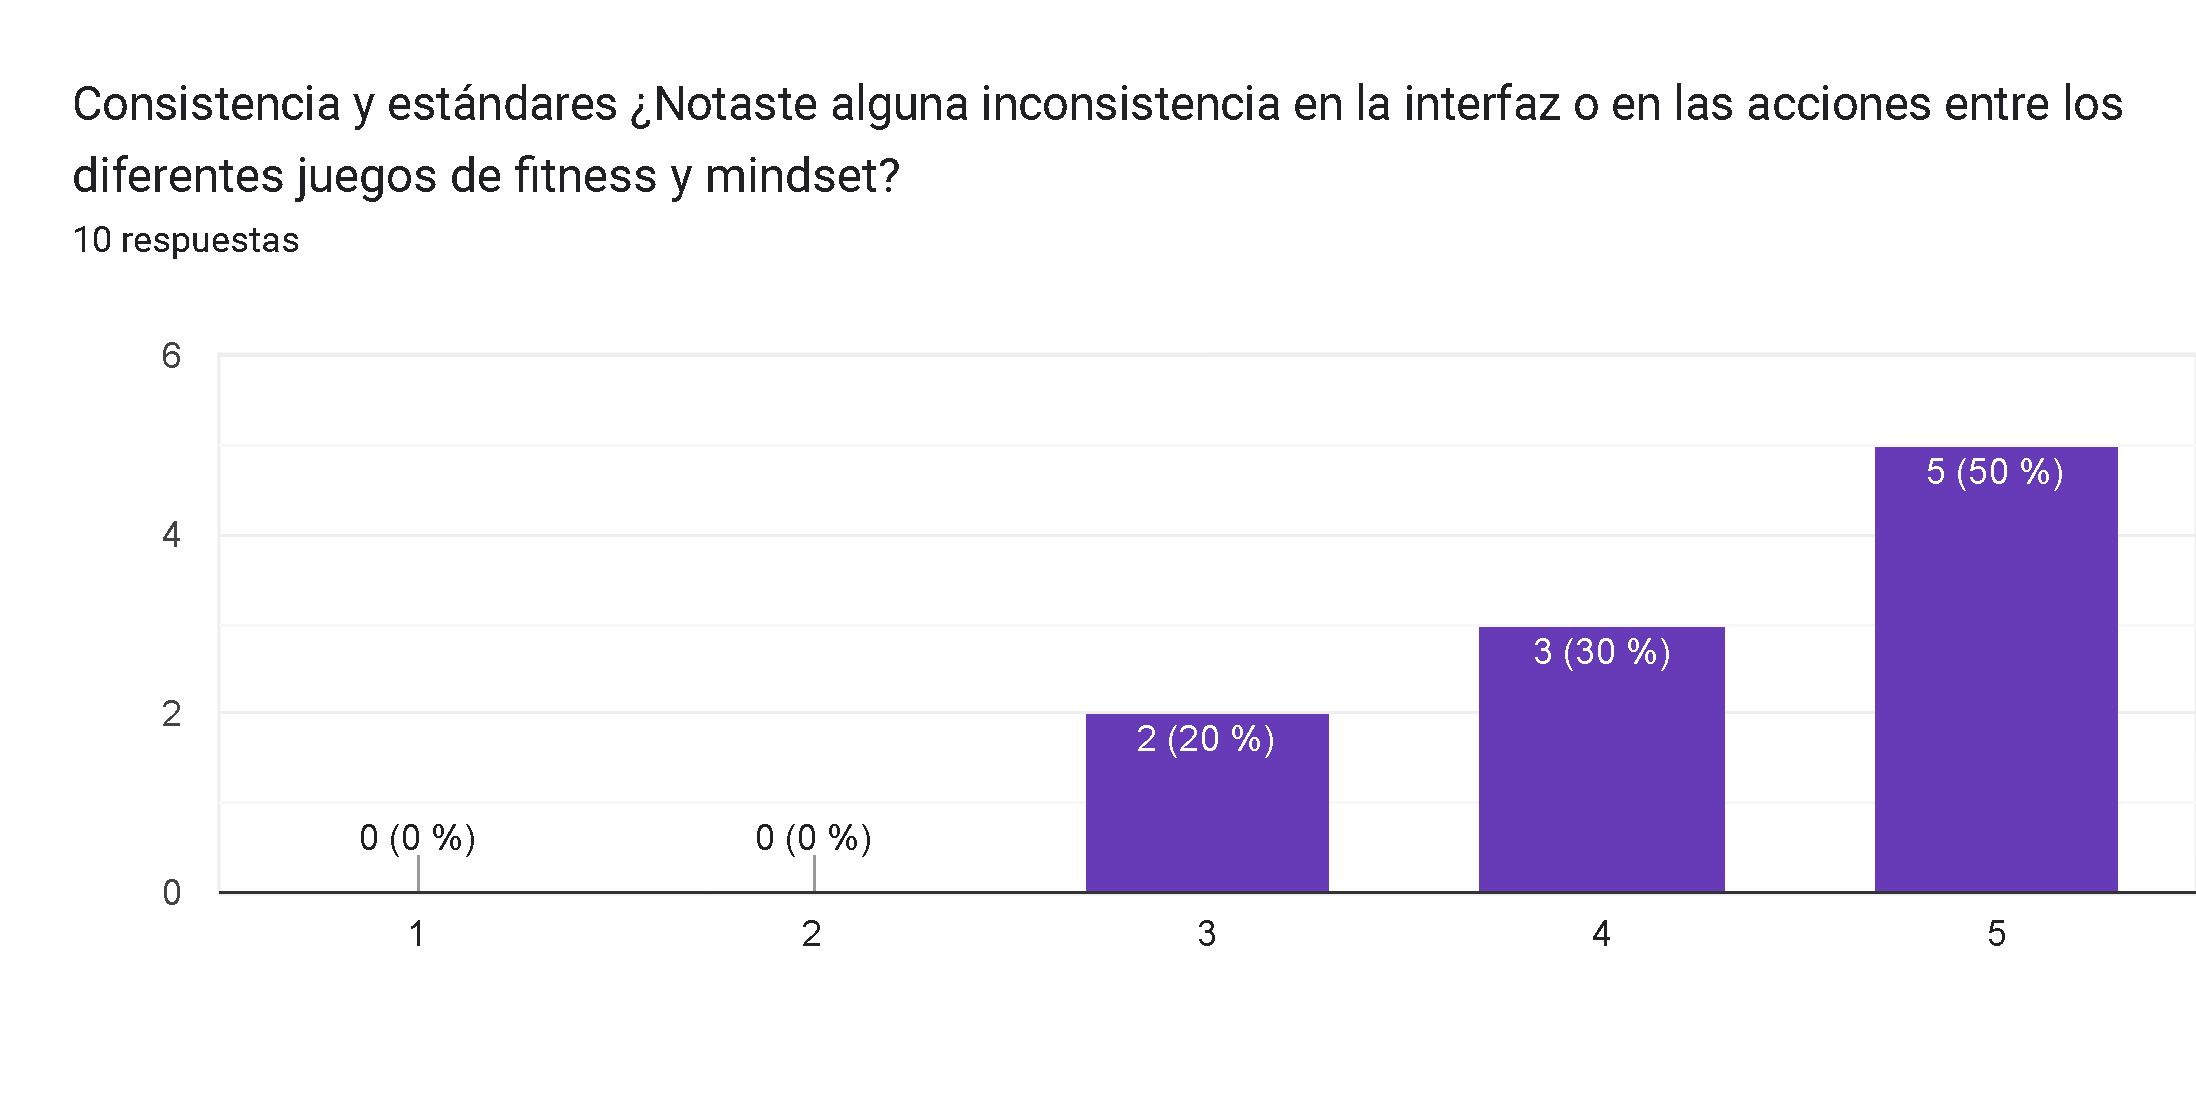
\includegraphics[width=0.7\linewidth]{Imagenes/Nc4.png}
  \caption{Elaboración propia, Imagen de referencia de cuestionario sobre pruebas de usabilidad heurísticas de Nielsen para plataforma gamificada sobre módulos Mindset y Fitness, `¿Notaste alguna inconsistencia en la interfaz o en las acciones entre los diferentes juegos de fitness y mindset?'}

  \label{fig:cuestionario4nielsen}
\end{figure}

La pregunta ``¿Te resultó claro qué acciones evitar o cuáles podrían causar problemas, como pausas incorrectas en los juegos o abandonos accidentales?'' obtuvo la mayor cantidad de respuestas en la opción 5, con un 40\%. Esto indica que la mayoría de los usuarios consideró que las acciones a evitar eran claras y entendidas correctamente. Un 30\% de los usuarios eligió la opción 4, lo que sugiere que la mayoría también encontró estas acciones claras, pero algunos podrían haber tenido dudas o dificultades menores en este aspecto. Un 20\% seleccionó la opción 3, lo que implica que una pequeña parte de los usuarios no encontró completamente claro qué acciones podrían causar problemas, y un 10\% eligió la opción 2, lo que señala que un pequeño grupo de usuarios experimentó confusión o falta de claridad en este aspecto.

\begin{figure}[H]
  \centering
  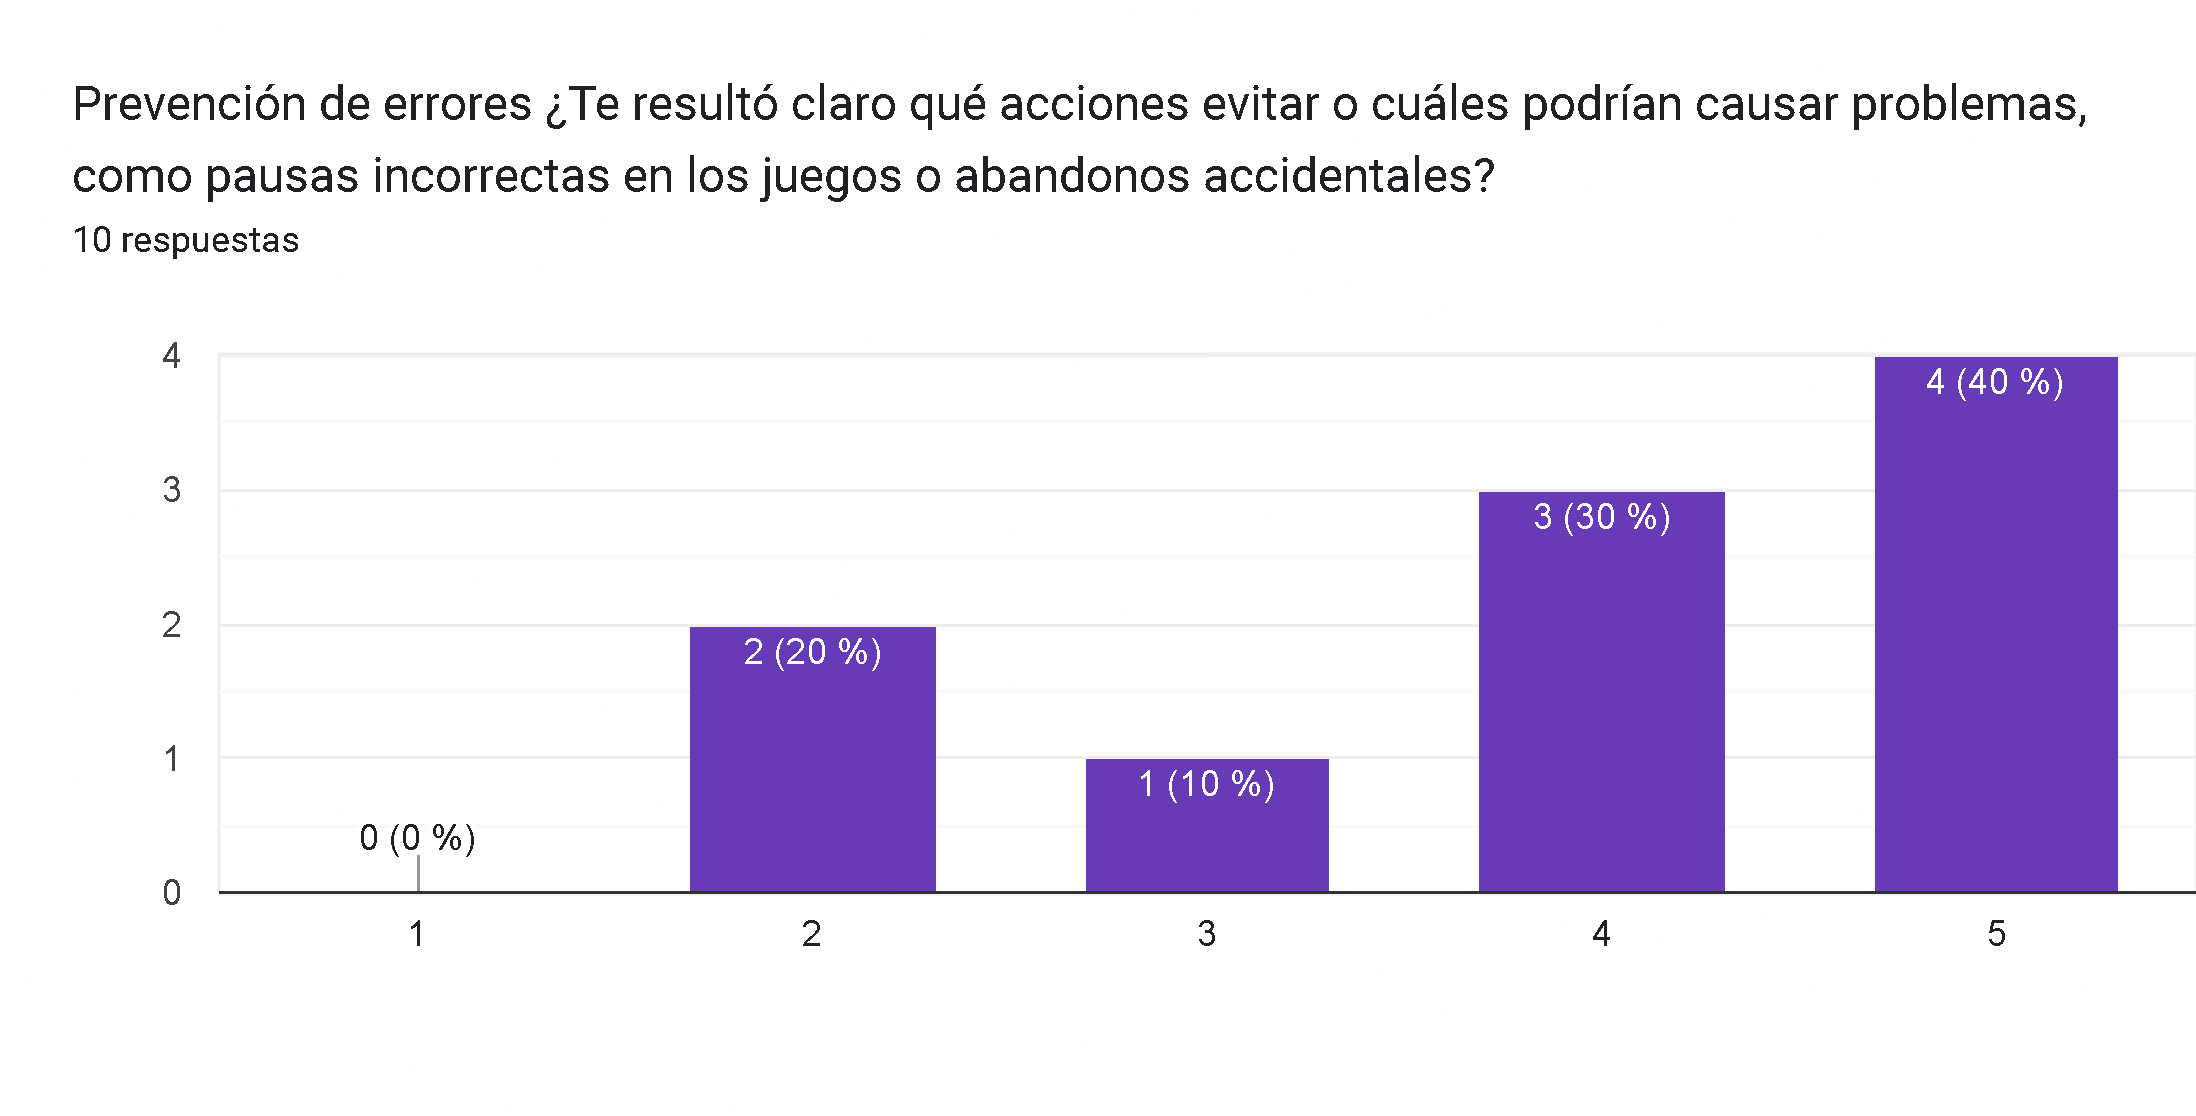
\includegraphics[width=0.7\linewidth]{Imagenes/Nc5.png}
  \caption{Elaboración propia, Imagen de referencia de cuestionario sobre pruebas de usabilidad heurísticas de Nielsen para plataforma gamificada sobre módulos Mindset y Fitness, `¿Te resultó claro qué acciones evitar o cuáles podrían causar problemas, como pausas incorrectas en los juegos o abandonos accidentales?'}

  \label{fig:cuestionario5nielsen}
\end{figure}

La pregunta ``¿Te fue fácil recordar cómo jugar y navegar en los juegos de fitness y mindset después de usarlos una vez?'' obtuvo la mayor cantidad de respuestas en la opción 5, con un 40\%. Esto indica que la mayoría de los usuarios encontraron fácil recordar cómo jugar y navegar en los juegos después de una sesión. Un 30\% de los usuarios eligió la opción 4, lo que sugiere que aunque la mayoría tuvo una buena experiencia recordando las acciones, algunos podrían haber tenido pequeñas dificultades. Un 20\% seleccionó la opción 3, lo que señala que un grupo de usuarios experimentó algo de dificultad al recordar cómo jugar, y un 10\% eligió la opción 2, lo que indica que una minoría encontró complicado recordar las acciones del juego.

\begin{figure}[H]
  \centering
  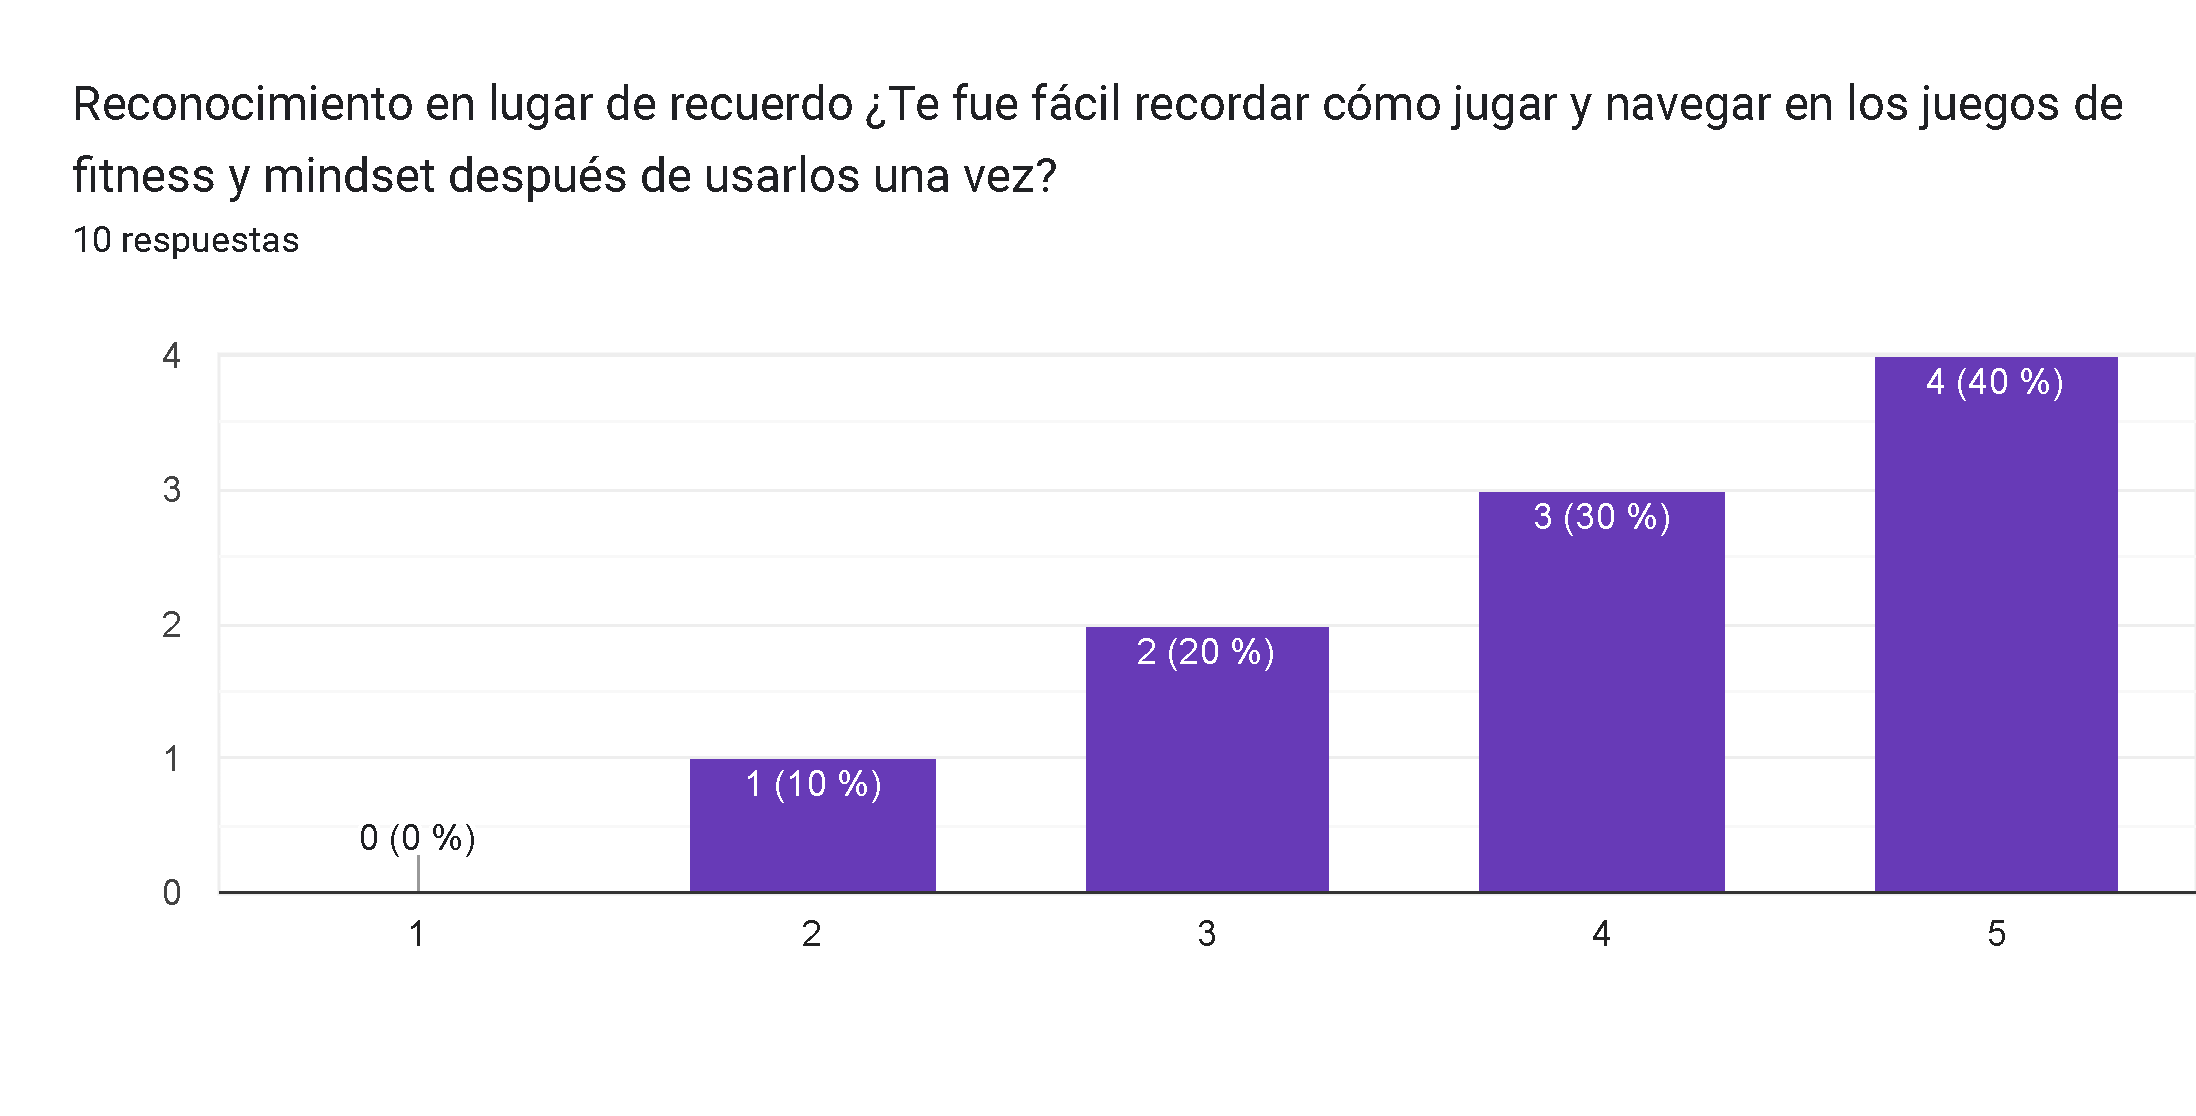
\includegraphics[width=0.7\linewidth]{Imagenes/Nc6.png}
  \caption{Elaboración propia, Imagen de referencia de cuestionario sobre pruebas de usabilidad heurísticas de Nielsen para plataforma gamificada sobre módulos Mindset y Fitness, `¿Te fue fácil recordar cómo jugar y navegar en los juegos de fitness y mindset después de usarlos una vez?'}

  \label{fig:cuestionario6nielsen}
\end{figure}

La pregunta ``¿Pudiste realizar acciones de manera eficiente, como cambiar entre diferentes juegos sin tener que seguir muchos pasos?'' obtuvo la mayor cantidad de respuestas en la opción 3, con un 50\%. Esto sugiere que la mayoría de los usuarios pudieron realizar acciones de manera eficiente, aunque algunos podrían haber encontrado que el proceso no fue completamente fluido. Un 20\% de los usuarios eligieron la opción 4, lo que indica que se sintieron aún más cómodos realizando las acciones, pero un 20\% seleccionó la opción 5, lo que sugiere que experimentaron cierta incomodidad. Solo un 10\% de los usuarios eligió la opción 1, lo que indica que una pequeña proporción encontró difícil realizar las acciones de manera eficiente.

\begin{figure}[H]
  \centering
  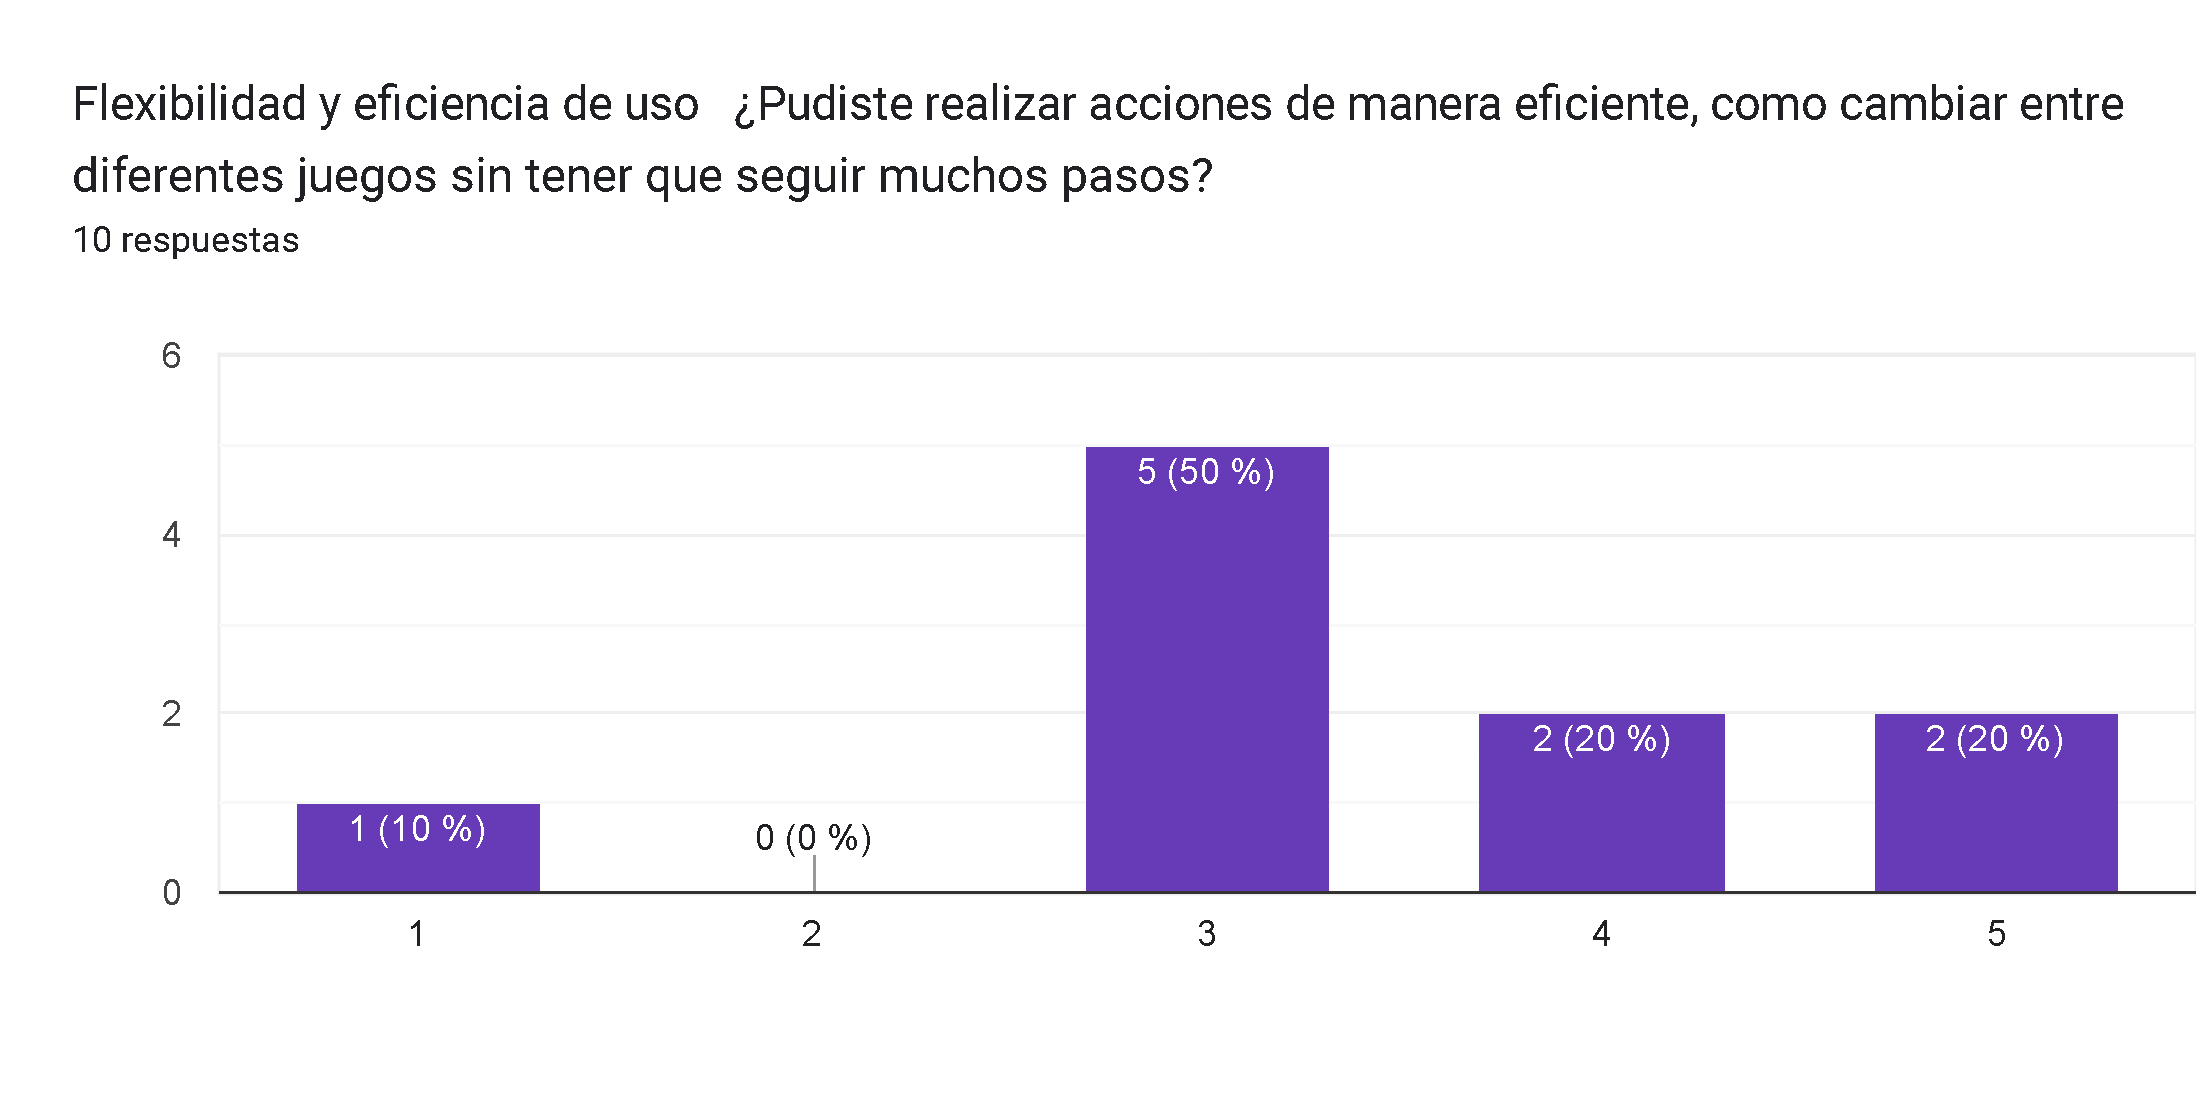
\includegraphics[width=0.7\linewidth]{Imagenes/Nc7.png}
  \caption{Elaboración propia, Imagen de referencia de cuestionario sobre pruebas de usabilidad heurísticas de Nielsen para plataforma gamificada sobre módulos Mindset y Fitness, `¿Pudiste realizar acciones de manera eficiente, como cambiar entre diferentes juegos sin tener que seguir muchos pasos?'}

  \label{fig:cuestionario7nielsen}
\end{figure}

La pregunta ``¿El diseño de los juegos y la plataforma te pareció limpio, intuitivo y libre de elementos innecesarios que pudieran distraer durante las sesiones de fitness o mindset?'' obtuvo la mayor cantidad de respuestas en la opción 5, con un 50\%. Esto sugiere que la mayoría de los usuarios encontraron el diseño limpio e intuitivo, sin elementos que distrajeran durante las sesiones. Un 30\% de los usuarios seleccionaron la opción 3, lo que indica que algunos consideraron que el diseño era limpio, pero podría mejorarse ligeramente. Un 20\% eligió la opción 2, lo que señala que algunos usuarios experimentaron distracciones menores debido al diseño de la plataforma.

\begin{figure}[H]
  \centering
  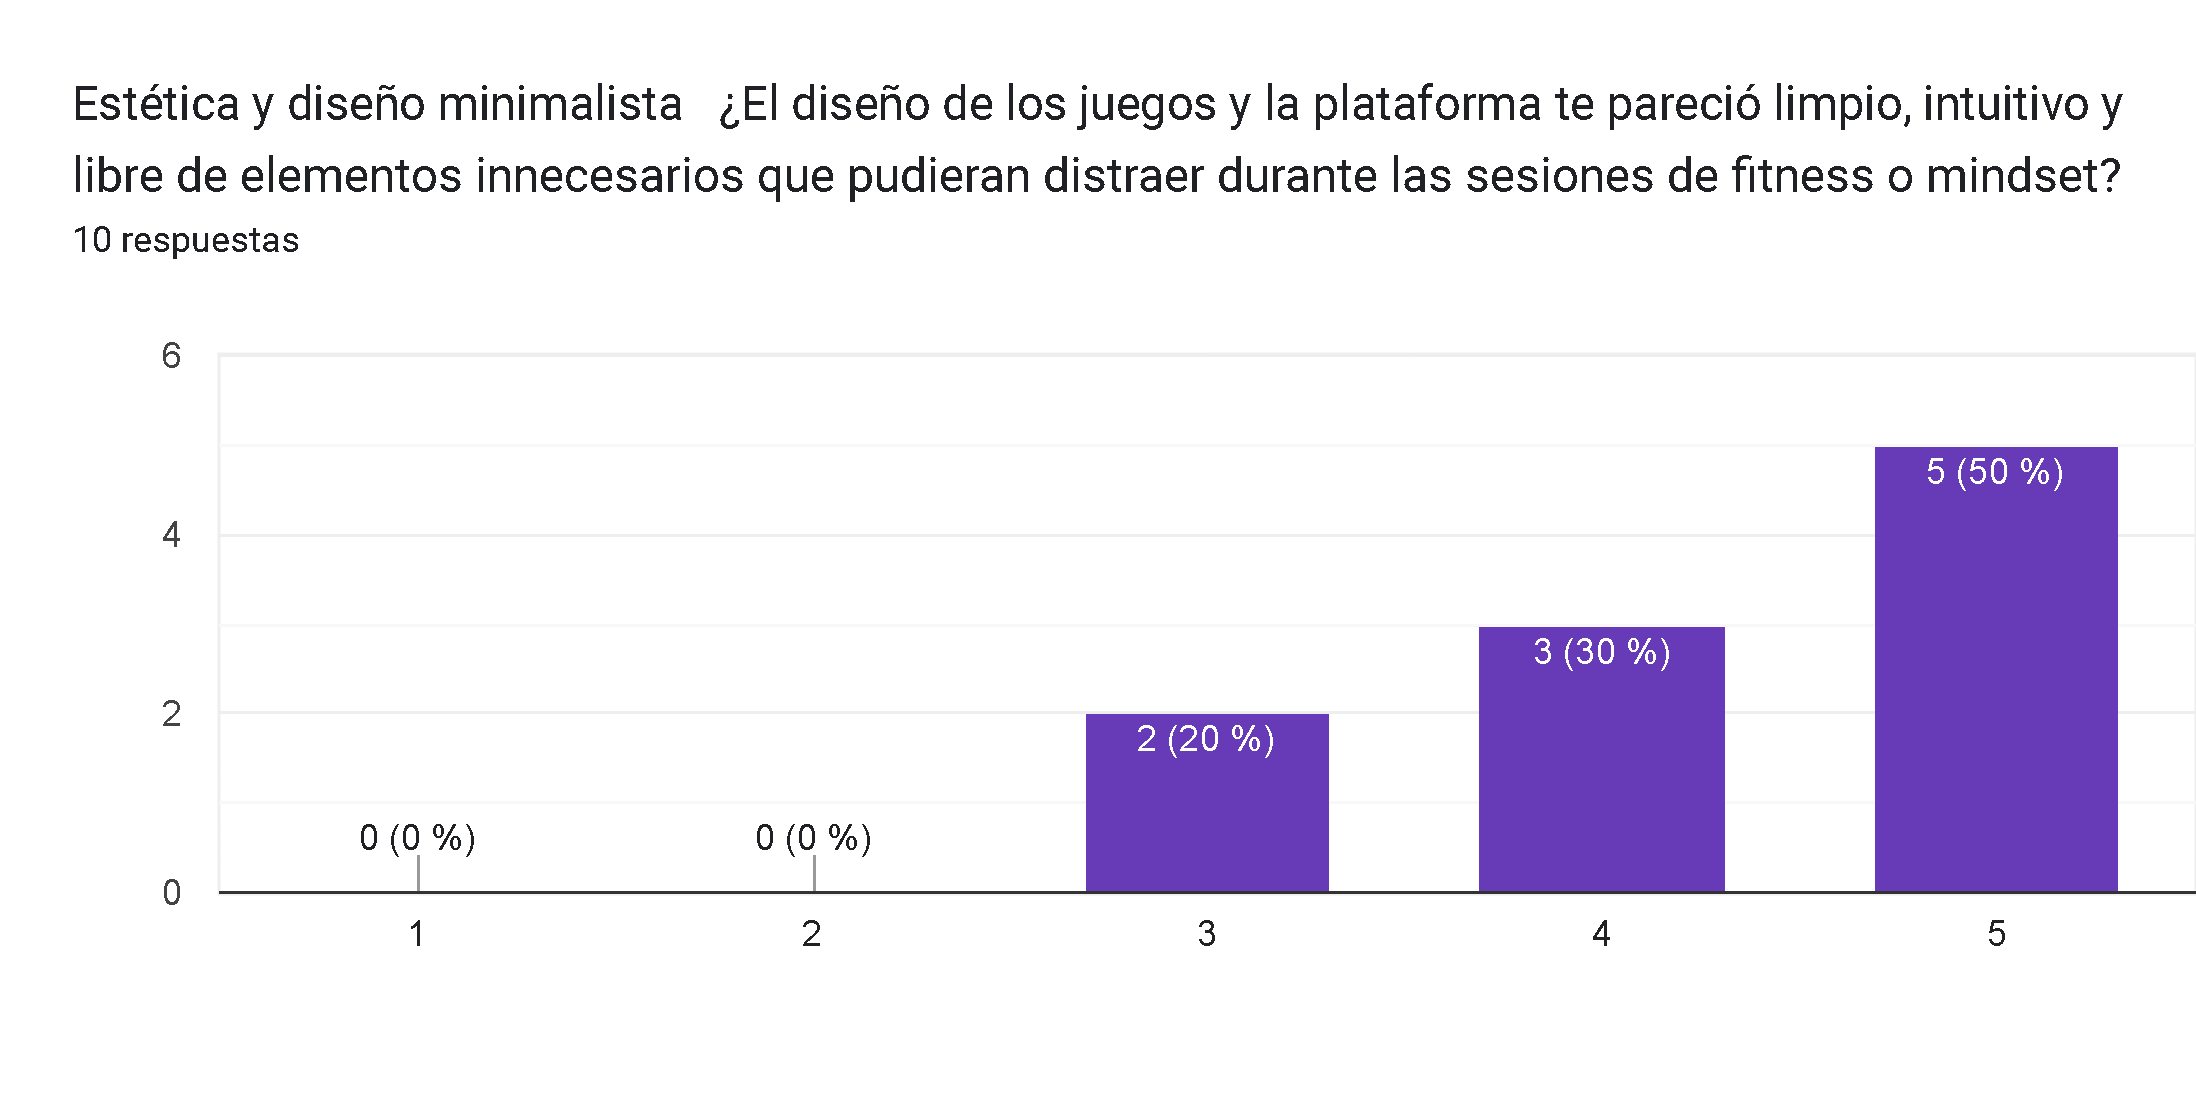
\includegraphics[width=0.7\linewidth]{Imagenes/Nc8.png}
  \caption{Elaboración propia, Imagen de referencia de cuestionario sobre pruebas de usabilidad heurísticas de Nielsen para plataforma gamificada sobre módulos Mindset y Fitness, `¿El diseño de los juegos y la plataforma te pareció limpio, intuitivo y libre de elementos innecesarios que pudieran distraer durante las sesiones de fitness o mindset?'}

  \label{fig:cuestionario8nielsen}
\end{figure}
